\chapter{Combination of dark matter searches interpreted in \thdma}
\label{chap:combination-dark-matter-2hdma}


\section{Theoretical considerations}
\label{sect:theoretical-considerations-2hdma}
The benchmark model used to interpret the data extends the Standard Model with a second complex Higgs doublet, already postulated in several UV-complete BSM theories \cite{Buckley:2014fba,Abercrombie:2015wmb}. After electroweak symmetry breaking, the model contains 5 Higgs bosons: a light CP-even boson $h$, a heavier CP-even boson $H$, a CP-odd boson $A$ and a two charged bosons $H^{\pm}$. The 2HDM allows some freedom in the choice of Higgs-fermion coupling structure, for example, 2HDM type-I which couples only one Higgs doublet to fermions, and 2HDM type-II, which couples the neutral member of one Higgs doublet to only up-type quarks and the neutral member of the other to down-type quarks. This search assumes the type-II structure, along with the alignment and decoupling limits, so that the lighter CP-even states $h$ can be identified with the SM Higgs boson \cite{Gunion:2002zf}. The Lagrangian of the 2HDM can be written as 
\begin{equation}
    \label{4.1}
    \mathcal{L}_{2HDM} = (D_{\mu}\Phi_1)^{\dag}(D^{\mu}\Phi_1) + (D_{\mu}\Phi_2)^{\dag}(D^{\mu}\Phi_2) - V(\Phi_1, \Phi_2)
\end{equation}
where the covariant derivative $D_{\mu}$ is given by 
$$D_{\mu} = \partial_{\mu} - ig\frac{\tau^i}{2}W^i_{\mu} - i\frac{g'}{2}YB_{\mu},$$
in which $\tau^i$ are Pauli matrices and $Y$ is the hypercharge. The potential is
\begin{equation} \label{4.2}
    \begin{split} 
        V(\Phi_1, \Phi_2)  &= m_{11}^2\Phi_1^{\dag}\Phi_1 + m_{22}^2\Phi_2^{\dag}\Phi_2 - (m_{12}^2 \Phi_1^{\dag}\Phi_2 + h.c.) \\
        &+ \frac{\lambda_1}{2}(\Phi_1^{\dag}\Phi_1)^2 + \frac{\lambda_2}{2}(\Phi_2^{\dag}\Phi_2)^2  
        + \lambda_3(\Phi_1^{\dag}\Phi_1)(\Phi_2^{\dag}\Phi_2) + \lambda_4 (\Phi_1^{\dag}\Phi_2)(\Phi_2^{\dag}\Phi_1) \\ 
        &+ \left\{ \frac{\lambda_5}{2} (\Phi_1^{\dag}\Phi_2)^2 + [\lambda_6(\Phi_1^{\dag}\Phi_1) + \lambda_7(\Phi_2^{\dag}\Phi_2) ](\Phi_1^{\dag}\Phi_2) + h.c. \right\} 
    \end{split}
\end{equation}
The scalar field vacuum expectation values occur at 
\begin{equation}
    \label{4.3}
    \expval{\Phi_i} = \frac{1}{\sqrt{2}}\begin{pmatrix}
        0 \\ v_i
    \end{pmatrix},\quad v_i \in \mathbb{R},
\end{equation}
with the following conditions
\begin{equation}
    \label{4.4}
    \begin{split}
        m_{11}^2 &= m_{12}^2 t_{\beta} - \frac{1}{2}v^2(\lambda_1  c^2_{\beta} + \lambda_{345} s^2_{\beta} + 3\lambda_6 s_{\beta} c_{\beta} + \lambda_7  s^2_{\beta} t_{\beta})  \\
        m_{22}^2 &= m_{12}^2( t_{\beta})^{-1} - \frac{1}{2}v^2(\lambda_2  s^2_{\beta} + \lambda_{345} c^2_{\beta} + \lambda_6 c^2_{\beta}( t_{\beta})^{-1} + 3\lambda_7  s_{\beta} c_{\beta}  ),
    \end{split}
\end{equation}
where 
$$ t_{\beta}=\frac{v_2}{v_1}, \quad \lambda_{345} = \lambda_3+\lambda_4+\lambda_5, \quad v = \sqrt{v_1^2 + v_2^2} = 246\, \mathrm{GeV}$$
After spontaneous symmetry breaking, three of the original eight scalar degrees of freedom are absorbed by the $W^{\pm}$ and the $Z$ bosons, leaving five physical Higgs bosons as described above. The physical masses of the CP-odd and charged Higgs states are given by 
\begin{equation}
    \label{4.5}
    \begin{split}
        m^2_{A} &= \frac{m_{12}^2}{ s_{\beta} c_{\beta}} - \frac{v^2}{2}\left( 2\lambda_5 + \frac{\lambda_6}{ t_{\beta}} + \lambda_7  t_{\beta}  \right) \\ 
        m^2_{H^{\pm}} &= m_{A}^2 + \frac{v^2}{2}(\lambda_5 - \lambda_5)
    \end{split}
\end{equation}
The two CP-even Higgs states mix according to the squared-mass matrix 
\begin{equation}
    \label{4.6}
    \mathbf{M}^2 = m^2_{A}\begin{pmatrix}
         s^2_{\beta} & - s_{\beta}  c_{\beta} \\
        - s_{\beta} c_{\beta} &  c^2_{\beta} 
    \end{pmatrix} + \mathbf{B}^2
\end{equation}
where
$$\mathbf{B}^2 = v^2\begin{pmatrix}
    \lambda_1 c^2_{\beta} + 2 \lambda_6 s_{\beta} c_{\beta} + \lambda_5 s^2_{\beta}  & (\lambda_3+\lambda_4) s_{\beta} c_{\beta} + \lambda_6 c^2_{\beta} + \lambda_7  s^2_{\beta} \\
    (\lambda_3 + \lambda_4) s_{\beta} c_{\beta} + \lambda_6 c^2_{\beta} + \lambda_7 s^2_{\beta} & \lambda_2 s^2_{\beta} + 2 \lambda_7 s_{\beta} c_{\beta} + \lambda_5 c^2_{\beta} 
\end{pmatrix}.$$
Diagonalizing $\mathbf{M}^2$ furnishes the physical CP-even Higgs states, whose squared-masses are the eigenvalues
\begin{equation}
    \label{4.7}
    m^2_{H,h} = \frac{1}{2}\left[ \mathbf{M}^2_{11} + \mathbf{M}^2_{22} \pm \sqrt{(\mathbf{M}^2_{11} - \mathbf{M}^2_{22})^2 + 4\mathbf{M}^2_{12}} \right],
\end{equation}
and the mixing angle 
\begin{equation}
    \label{4.8}
    s_{2\alpha} = \frac{2\mathbf{M}^2_{12}}{\sqrt{(\mathbf{M}^2_{11} - \mathbf{M}^2_{22})^2 + 4\mathbf{M}^2_{12}}} , \quad c_{2\alpha} = \frac{(\mathbf{M}^2_{11} - \mathbf{M}^2_{22})^2}{\sqrt{(\mathbf{M}^2_{11} - \mathbf{M}^2_{22})^2 + 4\mathbf{M}^2_{12}}}.
\end{equation}
The 2HDM, though being a BSM model, does not natively contain a dark sector. Therefore, a fermionic dark matter particle $\chi$ is included, and connected to the 2HDM sector by a pseudo-scalar CP-odd mediator $a$, with Yukawa-like couplings to both SM and DM fermions. The mediator mixes with the pseudo-scalar $A$ of the 2HDM with a mixing angle $\theta$. 

With the inclusion of the fermionic dark matter and the pseudo-scalar mediator, the phenomenology of the model is fully determined by 14 independent parameters:
\begin{enumerate}
    \item the mass of Higgs bosons $m_h$, $m_H$, $m_A$, $m_{H^{\pm}}$,
    \item the mass of the pseudo-scalar mediator $m_a$,
    \item the mass of the dark matter particle $\mchi$,
    \item the Yukawa coupling $g_{\chi}$ between $a$ and $\chi$,
    \item the electroweak VEV $v$,
    \item the ratio of the VEVs of the two Higgs doublets $\tanb$,
    \item the mixing angle $\alpha$ of the CP-even Higgs states $h$ and $H$,
    \item the mixing angle $\theta$ of the CP-odd states $A$ and $a$,
    \item the quartic coupling $\lambda_3$ of the pure 2HDM potential,
    \item the quartic couplings of the potential terms between the doublet and singlet fields $\lambda_{P1}$, and $\lambda_{P2}$
\end{enumerate}
Some of these parameters are constrained by electroweak and flavour measurements, as well as phenomenological considerations \cite{Bauer:2017ota,2HDMWGproxi}. Some parameters are chosen to simplify the model and reduce the space of independent parameters. Reference \cite{2HDMWGproxi} contains detailed descriptions of the \thdma benchmark scenarios recommended by the LHC Dark Matter working group. 

In this analysis, a total of 5 parameters are scanned over, including $m_A$, $m_a$, $\tanb$, $\sint$, and $\mchi$. Other parameters are set to constant in all benchmark scenarios. The coupling $g_{\chi}$ is set to $1$, having negligible effect on the shape of the kinematic distribution of interest. The alignment and decoupling limits are assumed, effectively assigning $m_h=125$ Gev, $v=246$ GeV, and $\cos(\beta-\alpha)=0$. The quartic coupling $\lambda_3$ is set to 3 to guarantee the stability of the Higgs potential for the chosen range of the heavy Higgs bosons. In addition, they are fixed to the same value, i.e. $m_A= m_H=m_{H^{\pm}}$. The heavy CP-even Higgs $H$ is chosen to have the same mass as the charged Higgs to avoid the constraints from electroweak precision measurements, and the same mass as the CP-odd Higgs to reduce the number of independent parameters \cite{Bauer:2017ota}. The other quartic couplings are also fixed at 3 to maximize the trilinear couplings between the CP-odd and the CP-even neutral sates. 

The phenomenology of the \thdma is particularly rich, and this analysis combines an unprecedented number of signatures as illustrated in table \ref{tab:input_summary}.
These signatures can be broadly categorized into those involving invisible and visible mediator decays, the former being represented by $\met+X$. An overview of the signatures considered are given in section \ref{sect:exp-signatures}, and further details can be found in the referenced publications. The dominant production mode for the majority of signatures is $gg$-initiated production. 
Figures \ref{subfig:zll-gg-fusion-res}, \ref{subfig:zll-gg-fusion-nonres} respectively summarize $gg$-initiated resonant and non-resonant production mechanisms of the $\monozll$ final state. 
Similarly, the $\monohbb$ signature, as well as other $\met+h$ signatures, can be produced both resonantly and non-resonantly via $gg$ fusion, as seen on figures \ref{subfig:hbb-gg-fusion-res} and \ref{subfig:hbb-gg-fusion-nonres}. 
In addition, $gg$-initiated production of the $\monojet$ signature is shown in figures \ref{subfig:metj-gg-fusion}, and $t\bar{t}$- or $b\bar{b}$-associated resonant $A/H$ production leading to $t\bar{t}t\bar{t}$, $b\bar{b}b\bar{b}$, $t\bar{t}b\bar{b}$, $\met+t\bar{t}$, or $\met+b\bar{b}$ signatures in Figure \ref{fig:tttt-signature}. 
Figure \ref{fig:tbHtb-signature} shows the production of a charged Higgs associated with and decaying into a pair of $tb$ quarks, designated $\htb$, and figure \ref{fig:haaff-signature} shows loop-induced Higgs production of a SM Higgs boson decaying into a pair of mediators $aa$ resulting in 2 pairs of fermionic DM or SM particles. 

The second largest production mode is $bb$-initiated production, whose primary signatures include $\monozll$, $\monohbb$, and $\monojet$. Representative Feynman diagrams are respectively shown in in figures \ref{subfig:zll-bb-associated}, \ref{subfig:hbb-bb-initiated}, \ref{subfig:metj-bb-associated}. Finally, the leading diagram for the $\met+tW$ signature is shown in figure \ref{fig:tW-signature}. The interplay between these signatures depends on the \thdma model parameters. 

\section{Benchmark scenarios}
\label{sect:benchmark-scenarios}
The parameter space is examine through a total of 6 representative benchmark scenarios, in which one or two parameters are varied while the others are fixed. Table 1 summarizes these scenarios, demarcated to demonstrate the rich phenomenology of the \thdma and to examine the interplay between the signature described in the previous section.

\subsection{Scenario 1: Exploration of two \texorpdfstring{$m_a-m_A$}{TEXT} planes}\label{subsection:ma-mA-scan}
This scenario evaluates constraints on \thdma as a function of the pseudo-scalar masses $m_a$ and $m_A$, highlighting the complex dependence of the model phenomenology on the pseudo-scalar mass hierarchy, which governs the production and decay modes that are kinematically accessible and favoured. In this scan, $\tanb$ is fixed to 1.0 which favours couplings to up-type quarks, particularly the top quark, while the $a-A$ mixing angle is fixed to two values $\sint=0.35$ and $\sint=0.7$, and thus two parameter planes are explored. These angles respectively correspond to low and almost maximal mixing between the CP-odd Higgs and the pseudo-scalar mediator connected to the dark sector.

\subsection{Scenario 2: Exploration of two \texorpdfstring{$m_A-\tanb$}{TEXT} planes}\label{subsection:mA-tanb-scan}

The scenario evaluates the constraints while simultaneously varying $m_A$ and $\tanb$ for the same choices of mixing angle $\sint$ in \ref{subsection:ma-mA-scan}. The pseudo-scalar mass $m_a$ is fixed to 250 GeV, so as to kinematically prevent on-shell decays of the mediator into a pair of top quarks, and enlarge the branching ratio of the decay into the fermionic DM particle $a\rightarrow \chi\chi$ up to $100\%$. This benchmark scenario highlights the dependence of the couplings of the CP-odd Higgs $A$ on the value of $\tanb$ as a function of its mass. In particular, low values of $\tanb$ correspond to stronger coupling to up-type quarks, while higher values of $\tanb$ favour couplings to down-type quarks and charged leptons. In addition, it examines the interplay between $gg$-initiated, top-loop induced and $b\bar{b}$-initiated production modes. 

\subsection{Scenario 3: Exploration of two \texorpdfstring{$m_a-\tanb$}{TEXT} planes }\label{subsection:ma-tanb-scan}

Similar to \ref{subsection:mA-tanb-scan}, constraints on \thdma are evaluated as a function of the pseudo-scalar mass $m_a$ and Higgs doublet VEV ratio $\tanb$. The CP-odd Higgs mass is fixed at $m_A=600$ GeV, allowing for the decays $A\rightarrow t\bar{t}$ and favouring it at low $\tanb$. The value of $m_A$ is motivated by constraints on the mass of the charged Higgs $m_{H^{\pm}} = m_A$ derived from precision measurements of $B$-meson decays \cite{Misiak:2017bgg,Bauer:2017ota}. Two parameter planes corresponding to $\sint=0.35$ and $\sint=0.7$ are examined, similar to the previous scenarios.

\subsection{Scenario 4: Variation of the pseudo-scalar mixing angle \texorpdfstring{$\sint$}{TEXT} }
\label{subsection:sint-scan}
This benchmark scenario highlights the interplay between the $\met+Z$ and $\met+h$ signatures arising from invisible mediator decays, and signatures that probe visible mediator decays. The couplings $g_{Aha}$, $g_{HZa}$ which affect $\met+h$ and $\met+Z$ production scale with $\sint\cos\theta$ and $\sint$ respectively, and the coupling $g_{at\bar{t}}$ which plays a dominant role in the leading $\met+X$ production modes, scales with $\sint$. As $\sint\rightarrow 0$, the sensitivity of the $\met+X$ signatures vanishes. 

\subsection{Scenario 5: Variation of the Dark Matter mass \texorpdfstring{$\mchi$}{TEXT} }
\label{subsection:mchi-scan}
The value of $\mchi$ has a strong effect on parameters in cosmological dark matter models, such as the relic density, and on the sensitivity of direct and indirect detections of DM. This benchmark scenario provides a basis to compare the sensitivity of collider searches to those of non-collider experiments and cosmological observations in the context of \hdma. Constraints are evaluated by varying $\mchi$ and fixing other free parameters to $\sint=0.35$, $m_A=600$ GeV, $m_a=400$ GeV, and $\tanb=1.0$. A similar benchmark scenario was examined in reference \cite{2HDMWGproxi} under a different set of pseudo-scalar mass parameters, which is fully excluded by a previous ATLAS publication \cite{EXOT-2017-32},. The current choices of $m_a$ and $m_A$ represent an unexplored region in the parameter space. 

\subsection{Scenario 6: Variation of the \texorpdfstring{$m_a-\mchi$}{TEXT} }
\label{subsection:ma-mchi-scan}
This scenario illustrates the interplay between searches for invisible and exotic decays of the Higgs boson $h$ in the context of \hdma. Other free parameters are set to $\sint=0.35$ and $\tanb=1.0$ for consistency with other benchmark scans, and $m_A=1200$ to satisfy the constraint on the coupling $g_{haa}$ from measurements of the total Higgs boson decay width \cite{Argyropoulos:2022ezr}. This is a strong constraint for $m_a<m_h/2$, satisfied only be a relatively narrow range of $m_A$ in the chosen subspace of other free parameters.

In all benchmark scenarios, unless varied, the DM mass is fixed at $\mchi=10$ GeV to ensure a significant branching ratio for its decay from the pseudo-scalar $a$ for $m_a>100$ GeV. As long as $\mchi<m_a/2$, the value of $\mchi$ has little impact on the sensitivity of the searches considered in this analysis. Consequently, it is possible to match the observed relic density across a range of model parameter space through and appropriate choice of $\mchi$ without much effect on the experimental signatures.

Various theoretical constraints are considered in selecting the ranges of the parameters that are varied these benchmark scenarios. First, in some regions of the parameter space, the scalar potential is not bounded from below at large $m_A$, occurring, for example, in scenario 1a for $(m_A\gtrsim1250,m_a=100)$ GeV and $(m_A\gtrsim1550,m_a=1000)$ GeV. However, these constraints could be substantially relaxed if the quartic couplings take values closer to the perturbative limit or in more general 2HDM models \cite{2HDMWGproxi,Bauer:2017ota,Haisch:2018djm}. Therefore, they should not be understood as a strong limit on the the validity of the model predictions that were used to derive the exclusion contours. Second, given the parameter choices, the $aah$ coupling exceeds the unitary limit of $4\pi$ for large $m_A$, for instance, in scenario 1a, for $(m_A\gtrsim1250,m_a=100)$ GeV and $(m_A\gtrsim1550,m_a=1000)$ GeV. In this region, the width of the additional heavy Higgs bosons grows substantially and the theoretical predictions are subject to additional uncertainties from the treatment of the width. Therefore, regions where the relative width $\Gamma/m$ of at least one heavy Higgs boson or of the pseudo-scalar mediator $a$ exceeds $20\%$ are marked as shaded areas in the summary plots in Section \ref{subsection:ma-mchi-scan}. This conservative approach to large widths follows Ref \cite{EXOT-2017-32}.

Table \ref{tab:benchmarks} summarizes the benchmark scenarios examined in this analysis. Scenarios 1a, 3a, 4a, 4b, and 5 are recommended by the LHC Dark Matter Working Group and appeared in previous ATLAS analyses \cite{EXOT-2017-32}. This work considers in addition scenarios 1b, 2, 3b, and 6, which are motivated by the studies in references \cite{2HDMWGproxi,Pani:2017qyd,Argyropoulos:2022ezr}. In particular, the choice of $\sint=0.7$ or $\theta \approx \pi/4$ corresponds to maximal mixing in the pseudo-scalar sector and is relevant for the $\met+tW$ search, which was designed specifically for \thdma signal processes \cite{Pani:2017qyd}. Scenario 6 is included for the first time in this work to showcase the rich phenomenology of the model.

\begin{table}[h!]
\centering
\begin{tabular}{llcccccc}
\hline
\hline
\multicolumn{2}{l}{Scenario}   & \multicolumn{5}{c}{Fixed parameter values}  & Varied parameters \\
&        & \sint    &  \mA[\GeV] & \ma[\GeV] & \mchi[\GeV] & \tanb  &  \\

\hline
\multirow{2}{*}{1} & a &          $0.35$  &      --    &      --   & $10$ 	& $1.0$    &  \multirow{2}{*}{$(\ma ,m_A)$} \\
& b & $0.70$  &      --    &      --   & $10$       & $1.0$    & \\
\multirow{2}{*}{2} & a          & $0.35$  &      --    & $250$     & $10$       &     --        &  \multirow{2}{*}{$(m_A, \tanb)$} \\
& b & $0.70$  &      --    & $250$     & $10$       &      --        & \\
\multirow{2}{*}{3} & a          & $0.35$  & $600$      &      --   & $10$       &      --        & \multirow{2}{*}{$(m_a, \tanb)$} \\
& b & $0.70$  & $600$      &      --   & $10$       &      --        & \\
\multirow{2}{*}{4} & a          &     --  & $600$      & $200$     & $10$       & $1.0$  & \multirow{2}{*}{$\sint$} \\
& b &     --  & $1000$     & $350$     & $10$       & $1.0$  & \\
5                           &   & $0.35$  & $1000$      & $400$    & --         & $1.0$  & \mDM \\
6                           &   & $0.35$  & $1200$     &      --   & --         & $1.0$  & ($m_a$, $m_\chi$) \\
\hline
\hline
\end{tabular}
\caption{Summary of the parameter settings for the different \thdma benchmark scenarios explored in this summary.}
\label{tab:benchmarks}
\end{table}

This work also covers more production modes of the Higgs bosons and the pseudo-scalar mediator. In the previous summary of dark matter searches by ATLAS \cite{EXOT-2017-32}, only $gg$-initiated production was considered for the $\met+Z$ signatures, and for the $\met+h$ signatures, $b\bar{b}$-initiated production was considered only for $\tanb>10$. In contrast, all $\met$ signatures take into account $b\bar{b}$-initiated production, which is relevant for the $\met+Z$ and $\met+h$ signatures not only at large $\tanb$, where it is more important, but also at more intermediate values.

\section{Data and simulated event samples}

Proton--proton collision data collected with the ATLAS detector during the period 2015--2018 at center-of-mass energy $\sqrt{s}=13$~\TeV are used in the majority of analyses considered in this summary. The data sample is equivalent to an integrated luminosity of 139~\ifb after ensuring good operational conditions of all detector sub-systems and high-quality data \cite{DAPR-2018-01}.

Monte Carlo simulation is used to model relevant background processes and predictions of the \hdma. Details on MC generation of various background processes considered in this analysis can be found in the individual studies referenced in Section~\ref{sect:exp-signatures}. The \thdma benchmark is implemented in the Universal FeynRules Output (UFO) format~\cite{Degrande:2011ua} and is referred to as \texttt{Pseudoscalar\_2HDM} throughout this discussion.

\begin{table}[h!]
\centering
\scalebox{0.8}{
\begin{tabular}{p{26mm}p{90mm}p{16mm}p{26mm}}
\hline\hline
Analysis & Generator and Parton Shower & Cross-section & Further details \\
\toprule
\monozll  & \MGNLO 2.4.3 (LO) + \PYTHIA 8.212 & LO & \\
\monohbb  & \MGNLO 2.6.0 (LO) + \PYTHIA 8.212 & LO & \\
\monohgamgam  & \MGNLO 2.7.3 (LO) + \PYTHIA 8.244& LO & \\
\monohtautau  & \MGNLO 2.7.3 (LO) + \PYTHIA 8.244& LO & \\
$\met+j$  & \MGNLO 2.7.3 (LO) + \PYTHIA 8.244 & LO & Section~\ref{subsect:metj} \\
$\met+tW$ & \MGNLO 2.7.3 (LO) + \PYTHIA 8.244 & LO &  \\
%
\tttt     & \MGNLO 2.9.5 (LO) + \PYTHIA 8.245 & LO & reference~\cite{Bauer:2017ota} \\
\htb      & \MGNLO 2.2.2 (NLO) + \PYTHIA 8.212 & NLO, 4FS & Section~\ref{subsect:tbHtb}  \\
%
\hline
\hline
\end{tabular}
}
\caption{Details of the \MGNLO generation set-up used for the \thdma signal samples, for the signatures considered in this publication.
The \texttt{Pseudoscalar\_2HDM} UFO model is used for all simulated samples except those for the \htb search, which relies on the UFO of reference~\cite{Degrande:2015vpa}.
The \hinv\ and \hlrs signatures are not listed here as no signal samples required for the re-interpretation, which in those cases relies on the branching ratio limits.}
\label{tab:MCscalarsignal}
\end{table}

With the exception of the \htb process (Table~\ref{tab:MCscalarsignal}), all signal processes are generated at leading order (LO) in the strong coupling constant. In this context, LO corresponds to loop-induced gluon-gluon fusion for the $\met+X$ signatures, demonstrated for instance in figures \ref{subfig:zll-gg-fusion-res} and \ref{subfig:zll-gg-fusion-nonres}.

Event generation is performed using this UFO implementation with the \MGNLO~\cite{Alwall:2014hca} MC generator, which is interfaced with \PYTHIA8\cite{Sjostrand:2014zea} to simulate the parton shower and hadronization. The parameter settings follow the ATLAS tune A14~\cite{ATL-PHYS-PUB-2014-021}. Depending on the specific analysis, different versions of \MGNLO (ranging from 2.6.0 to 2.9.5) and \PYTHIA (from 8.212 to 8.245) were used, as summarized in Table~\ref{tab:MCscalarsignal}. These version differences are not expected to impact the signal simulations. The NNPDF3.0NLO~\cite{Ball:2014uwa} parton distribution function (PDF) set, based on next-to-leading-order calculations in the five-flavor scheme, was used, assuming a massless $b$-quark and $\alpha_{s}(m_{Z}) = 0.118$~\cite{Ball:2014uwa}.

To maintain consistency, the five-flavor scheme with $m_b = 0~\GeV$ was adopted for the matrix element (ME) computation in \MGNLO for $b\bar{b}$-initiated production. In contrast, the four-flavor scheme was used for $gg$-initiated production to incorporate top and bottom quark contributions in the production loop. These modelling choices align with the recommendations of the LHC Dark Matter Working Group~\cite{2HDMWGproxi}.

To account for pile-up effects from additional $pp$ collisions in the same or nearby bunch crossings, a number of interactions appropriate to the expected pile-up level of the data taking period were simulated using soft QCD processes in \PYTHIA8.186 with the A3 tune\cite{ATL-PHYS-PUB-2012-003} and the MSTW2008LO PDF~\cite{Martin:2009iq}. These interactions were overlaid onto each simulated hard-scatter event. The generated samples were reweighted to match the instantaneous luminosity distribution observed in data. The simulations also incorporate the expected bunch train structure and include corrections to address related effects.

Simulated events were processed using either a full detector simulation based on \GEANT~\cite{Agostinelli:2002hh, SOFT-2010-01} or a fast simulation\cite{ATL-PHYS-PUB-2010-013} that parametrizes the calorimeter response while relying on \GEANT for the rest of the detector. Physics objects in all simulated data samples were reconstructed from detector response following identical procedures as those applied on real data. Additionally, corrections derived from data control samples were applied to the simulations to account for differences between simulation and data in reconstruction efficiency, energy/momentum scale, and resolution of reconstructed electrons and muons. Analogous corrections were also made to account for differences in efficiency and false positive rate in the identification of jets containing $b$-hadrons. The energy scale and resolution of hadronic jets were adjusted to ensure consistency between data and simulation.

To efficiently generate signal events across the extensive multi-dimensional parameter space of the \hdma, the \mg~reweighting module~\cite{Mattelaer:2016gcx} was used to obtain predictions for various signal model parameters from a minimal set of generated events by assigning new event weights based on the ratio of matrix elements of the generated and target parameter points. These weights were computed dynamically during event simulation. The validity of this approach was confirmed by comparing weighted distributions with directly generated ones for select sample cases. This reweighting method significantly reduces computational costs, as detector simulation only needs to be performed once.

\section{Experimental signatures}
\label{sect:exp-signatures}

A total of 13 searches in different final states targeting invisible or visible mediator decays are included in this summary. No significant deviation from the SM predictions was observed in all searches, and instead they are used to derive constraints on the \thdma for the benchmark scenarios introduced in section \ref{sect:benchmark-scenarios}. Because the sensitivity of these searches varies across different regions of the \thdma parameter space, most of them are interpreted in a subset of the current benchmark scenarios. Table \ref{tab:input_summary} summarizes the scenarios in which each search is interpreted, and some details on each search are provided in this section. The searches using $\monohbb$, $\monozll$ and $\htb$ signatures enter a statistical combination described in section \ref{sect:stat}; limit contours from other relevant searches are overlaid on summary plots.

\begin{table}[h!]
\centering
%
%
\begin{tabular}{lccccccccccc}
\hline
\hline
Analysis/Scenario  & 1a & 1b & 2a & 2b & 3a & 3b & 4a & 4b & 5 & 6 \\
\midrule
\monozll~\cite{HIGG-2018-26} & x & x & x  & x  & x & x  & x  & x  & x  &     \\
\monohbb~\cite{EXOT-2018-46} & x & x & x  & x  & x & x  & x  & x  & x  & x   \\
\monohgamgam~\cite{HIGG-2019-02} & x & x &   &   & x & x & x & x &  &    \\
\monohtautau~\cite{HDBS-2018-50} & x &   &   & x &   &   &   &   &   &   \\
$\met+tW$~\cite{EXOT-2021-01} & x & x & x & x & x  & x  & x  & x  &   &   \\
$\met+j$~\cite{EXOT-2018-06} & x & x &   &  & x & x & x  & x  &   &   \\
\hinv~\cite{HIGG-2021-05} & x & x &   &   & x &   &   &   &   & x   \\
$\met+Z(q\bar{q})$~\cite{EXOT-2016-23} & x &  &   &   &  &   & x  & x  &    &     \\
$\met+\bbar$~\cite{SUSY-2016-18} &   &   &    &    &   &    & x  & x  &    &     \\
$\met+\ttbar$~\cite{SUSY-2016-18,SUSY-2016-16} &  &   &    &    &   &   & x  & x  &    &     \\
\tttt~\cite{EXOT-2019-26} & x & x & x & x & x & x & x & x & x &     \\
\htb~\cite{HDBS-2018-51}  & x & x & x & x & x & x & x & x & x &     \\
\hlrs~\cite{HDBS-2021-03,HIGG-2017-05,HIGG-2014-02,EXOT-2016-22,HDBS-2018-55}  &   &   &   &   &   &   &   &   &   & x   \\
\hline
\hline
\end{tabular}
%
\caption{Summary of input analyses used in the different benchmark scenarios.}
\label{tab:input_summary}
\end{table}

Each analysis targets a different signature and therefore relies on a different set of key physics objects identified by various subsystems of ATLAS. Jets are reconstructed from particle-flow objects using the anti-$k_t$ algorithm \cite{Cacciari:2008gp,Fastjet, PERF-2015-09}. The radius parameters are $R=0.4$ for small-$R$ jets and $R=1.0$ for large-$R$ jets \cite{JETM-2018-05}. Small-$R$ jets with $\abs{\eta}<2.5$ containing $b$-hadrons are identified with multivariate algorithms \cite{FTAG-2019-07,FTAG-2018-01}. Photons and electrons are reconstructed from topologically connected clusters of energy deposits in the electromagnetic (EM) calorimeters, with electron showers additionally matched to a charged-particle track in the Inner Detector (ID) \cite{EGAM-2018-01,ATL-PHYS-PUB-2017-022}. Muons are reconstructed by matching tracks in the ID and the muon spectrometer (MS), and refining through a global fit using hits from both sub-detectors\cite{PERF-2015-10}. Different lepton and photon selection criteria, and kinematic requirements are employed for particle identification and isolation in the analyses. $\tau$-lepton reconstruction relies on leptonic or hadronic $\tau$-lepton decay targeted by each analysis depending on the given signature \cite{ATL-PHYS-PUB-2015-045,ATLAS-CONF-2017-029}. The visible part of hadronically decaying $\tau$-leptons is seeded by small-$R$ jets reconstructed from topological clusters, calibrated with a hadronic weighting scheme \cite{Barillari:1112035}. The missing transverse momentum $p_T^{miss}$ is calculated from the negative vector sum of the transverse momenta $p_T$ of electrons, muons, jet candidates, and an additional soft term which includes activity in the tracking system originating from the primary vertex but not matched with any reconstructed particle \cite{PERF-2016-07}. Some analyses may also consider photons and $\tau$-leptons in the $\met$ reconstruction.

\subsection{\texorpdfstring{$\monozll$}{TEXT} signature}

\begin{figure}[h!]
    \centering
    \begin{subfigure}[b]{0.48\textwidth}
        \centering
        \begin{tikzpicture}
          \begin{feynman}
            \vertex (t1) at (0,0);
            \vertex (t2) at (-0.866, 0.5);
            \vertex (t3) at (-0.866, -0.5);
            \vertex [above left = of t2] (a);
            \vertex [below left = of t3] (b);
            \vertex [right = of t1] (c);
            \vertex [above right = of c] (d) {$Z$};
            \vertex [below right = of c] (e);
            \vertex [above right = of e] (f1) {$\chi$};
            \vertex [below right = of e] (f2) {$\chi$};

            \diagram[horizontal = t1 to c] {
                (t1) -- [scalar, edge label=\(H\)] (c),
                (t1) -- [fermion] (t3)  -- [fermion] (t2) --[fermion, edge label=\({t,b}\quad\,\,\)] (t1),
                (c) -- [photon] (d),
                (c) -- [scalar, edge label=\(a\)] (e),
                (e) -- [fermion] (f1),
                (e) -- [anti fermion] (f2),
                (a) -- [gluon] (t2),
                (b) -- [gluon] (t3),
            };
          \end{feynman}
        \end{tikzpicture}
        \vfill
        \caption{Gluon-gluon fusion resonant production}
        \label{subfig:zll-gg-fusion-res}
    \end{subfigure}
    \hfill
    \begin{subfigure}[b]{0.48\textwidth}
        \centering
        \begin{tikzpicture}
          \begin{feynman}
            \vertex (t1) at (0.134,0.4);
            \vertex (t4) at (0.134, -0.4);
            \vertex (t2) at (-0.866, 0.5);
            \vertex (t3) at (-0.866, -0.5);
            \vertex [above left = of t2] (a);
            \vertex [below left = of t3] (b);
            \vertex [right = of t1] (c);
            \vertex [above right = of t1] (d) {$Z$};
            \vertex (e) at (0.8, -0.6);
            \vertex [above right = of e] (f1) {$\chi$};
            \vertex [below right = of e] (f2) {$\chi$};

            \diagram[horizontal = t1 to c] {
                (t1) -- [fermion] (t4) --[fermion]  (t3) -- [fermion] (t2) --[fermion] (t1),
                (t1) -- [photon] (d),
                (t4) -- [scalar, edge label=\(a\)] (e),
                (e) -- [fermion] (f1),
                (e) -- [anti fermion] (f2),
                (a) -- [gluon] (t2),
                (b) -- [gluon] (t3),
            };
          \end{feynman}
        \end{tikzpicture}
        \vfill
        \caption{Gluon-gluon fusion non-resonant production}
        \label{subfig:zll-gg-fusion-nonres}
    \end{subfigure}
    \vfill
    \begin{subfigure}[b]{0.48\textwidth}
        \centering
        \begin{tikzpicture}
          \begin{feynman}
            \vertex (t1) at (0,0);
            \vertex (t2) at (-0.7, 1.5) {$\bar{b}$};
            \vertex (t3) at (-0.7, -1.5) {$b$};
            \vertex (t4) at (1, 0.2);
            \vertex (t5) at (3, 1.5) {$Z$};
            \vertex (t6) at (1.5, -1) ;
            \vertex (t7) at (2.7, -0.5) {$\bar{\chi}$};
            \vertex (t8) at (2.7, -1.8) {$\chi$};
            \diagram[] {
                (t1) -- [fermion] (t2),
                (t3) -- [fermion] (t1),
                (t1) -- [scalar, edge label = \(H\)] (t4),
                (t4) -- [photon] (t5),
                (t4) -- [scalar, edge label = \(a\)] (t6),
                (t7) -- [fermion] (t6),
                (t6) -- [fermion] (t8),
            };
          \end{feynman}
        \end{tikzpicture}
        \caption{$b\bar{b}$-initiated production}
        \label{subfig:zll-bb-associated}
    \end{subfigure}
    \caption{Representative production mechanisms and final state of the $\monozll$ signature, including gluon-gluon fusion resonant (a) and non-resonant production, and (c) $b$-initiated production.}
    \label{fig:zll-signature}
\end{figure} 

The final state of this signature, shown on figure \ref{fig:zll-signature}, is characterized by the presence of a large $\met$ and a pair of high-$p_T$ electrons or muons \cite{HIGG-2018-26}. Signal events must contain exactly a pair of oppositely charged electrons or muon, with an invariant mass consistent with the $Z$-boson mass. The leptons are order in increasing $p_T$. The leading lepton is required to have $p_T > 30$ GeV, and the sub-leading lepton $p_T>20$ GeV. The dilepton system must have an invariant mass $m_{ll}$ in the range $76 < m_{ll} < 106$ GeV, in accordance with the mass of the $Z$ boson. The missing transverse momentum is required to have $\met>90$ GeV, and a $\met$ significance $S_{\met}=\frac{\met}{\sigma_L\sqrt{1-\rho_{LT}^2}}>0$, in which $\sigma_L$ denotes the resolution of the $pT$ of the system and $\rho_{LT}$ a correlation factor between the resolutions of the parallel and perpendicular momentum components of the $\met$ vector \cite{ATLAS-CONF-2018-038}. These quantities are calculated from MC simulation and shown to well describe the data. The requirements of $\met$, in addition to the constraints that the angular separation between the leptons $\Delta R_{ll}<1.8$ ensure consistence with invisible particles recoiling against the $Z$ boson. 

The most abundant background is diboson production $ZZ$, followed by $WZ$, $Z+j$, and non-resonant backgrounds ($WW$, $t\bar{t}$, single top-quark, $Z\rightarrow\tau\tau$). Additional backgrounds come from triboson production, $t\bar{t}+V$, and $ZZ\rightarrow 4l$, where a pair of leptons is not reconstructed. 

The $ZZ$ background is estimated from MC simulation using a 4-lepton control region (CR), which is almost $100\%$ pure in $ZZ$ events. Events are required to contain two lepton pairs of the same flavour, opposite charge, and $p_T>7,\,15,\,15,\,27$ GeV in increasing order of $p_T$. If all  leptons in the final state are of the same flavour, they are grouped in pair by minimizing the quantity $\abs{m_{ll1} - m_Z} + \abs{m_{ll2} - m_Z}$, where the indices $1$ and $2$ denote the lepton pairs and $m_Z=91.19$ GeV. Similar to the signal region (SR), both lepton pairs must have $76<m_{ll} < 106$ GeV. The quantities $\met$ and $S_{\met}$ are calculated similarly as in the SR by treating a random pair of leptons as invisible and excluded from the calculation.

The $WZ$ background is constrained by a 3-lepton CR, in which two of the leptons have the same flavour and opposite charge to ensure their origin from a $Z$ boson. This dilepton system, when ordered by increasing $p_T$ must satisfy $p_{T}^1>20$ GeV and $p_{T}^2>30$ GeV, and $76< m_{ll}< 106$ GeV. If there is ambiguity in selecting a dilepton pair, the pair closest to the $Z$ boson in invariant mass is selected. The select events consistent with a $W$ boson decay, the third lepton is required to have $p_T>20$ GeV, the event to have $\met>30$ GeV and $S_{\met}>3$, and the transverse mass of the $W$ boson candidate $m_T^W=\sqrt{2p_T^l\met(1-\cos\Delta\phi(l,E_R^{miss}))} > 60$ GeV, where $\Delta\phi(l, \met)$ is the azimuthal angle between the third lepton and the $\met$ momentum. 

Finally, the non-resonant background is constrained primarily by a $e\mu$ CR, defined similarly to the SR, with the exception of the lepton flavour requirement. This CR includes $t\bar{t}$, single top quark, $WW$ and $Z\rightarrow \tau\tau$ events. The remaining backgrounds are estimated from MC simulation. 

A profile likelihood fit in the $ee$ and $\mu\mu$ signal regions and the control regions is used to estimate the signal strength. In the SRs and the $e\mu$ CR, the observable of interest is the transverse mass
\begin{equation}
    \label{4.9}
    m_T^{lep}=\sqrt{\left[ \sqrt{m_Z^2+(p_T^{ll})^2} + \sqrt{m_Z^2+ (\met)^2} \right] ^2 - \left[ \mathbf{p}_T^{ll} + \mathbf{p}_T^{miss} \right]^2},\quad m_T^{lep}>200 \,\mathrm{GeV}
\end{equation}
while the $\met$ is used in the $4l$- and $3l$-CR. The transverse mass provides a good separation between the 2DHM+a signal and the $ZZ$ background. 

\subsection{\texorpdfstring{$\monohbb$}{TEXT} signature}

The final state of this signature, shown on figure \ref{fig:hbb-signature}, is characterized by a SM Higgs boson decaying into two $b$-jets and a significant $\met$ from the decay of the pseudo-scalar $a$ \cite{EXOT-2018-46}. Hence, selected events must contain at least two jets identified as $b$-jets and $\met>150$ GeV. The angular separation between the two $b$-jets is inversely proportional to the transverse momentum of the Higgs boson, which is highly correlated to $\met$; as such, at $\met>500$ GeV, the dijet system is reconstructed as a single large-radius jet. This motivates splitting the events into merged regions and resolved regions, according to the decay topology and thus $\met$. 

\begin{figure}
    \centering
    \begin{subfigure}[b]{0.48\textwidth}
        \centering
        \begin{tikzpicture}
          \begin{feynman}
            \vertex (t1) at (0,0);
            \vertex (t2) at (-0.866, 0.5);
            \vertex (t3) at (-0.866, -0.5);
            \vertex [above left = of t2] (a);
            \vertex [below left = of t3] (b);
            \vertex [right = of t1] (c);
            \vertex [above right = of c] (d) {$h$};
            \vertex [below right = of c] (e);
            \vertex [above right = of e] (f1) {$\chi$};
            \vertex [below right = of e] (f2) {$\chi$};

            \diagram[horizontal = t1 to c] {
                (t1) -- [scalar, edge label=\(A\)] (c),
                (t1) -- (t2) -- (t3) --[edge label=\({t,b}\quad\,\,\)] (t1),
                (c) -- [scalar] (d),
                (c) -- [scalar, edge label=\(a\)] (e),
                (e) -- [fermion] (f1),
                (e) -- [anti fermion] (f2),
                (a) -- [gluon] (t2),
                (b) -- [gluon] (t3),
            };
          \end{feynman}
        \end{tikzpicture}
        \vfill
        \caption{Gluon-gluon fusion production}
        \label{subfig:hbb-gg-fusion-res}
    \end{subfigure}
    \hfill
    \begin{subfigure}[b]{0.48\textwidth}
        \centering
        \begin{tikzpicture}
            \begin{feynman}
            \vertex (t1) at (0.134,0.4);
            \vertex (t4) at (0.134, -0.4);
            \vertex (t2) at (-0.866, 0.5);
            \vertex (t3) at (-0.866, -0.5);
            \vertex [above left = of t2] (a);
            \vertex [below left = of t3] (b);
            \vertex [right = of t1] (c);
            \vertex [above right = of t1] (d) {$h$};
            \vertex (e) at (0.8, -0.6);
            \vertex [above right = of e] (f1) {$\chi$};
            \vertex [below right = of e] (f2) {$\chi$};

            \diagram[horizontal = t1 to c] {
                (t1) -- [fermion] (t4) --[fermion]  (t3) -- [fermion] (t2) --[fermion] (t1),
                (t1) -- [photon] (d),
                (t4) -- [scalar, edge label=\(a\)] (e),
                (e) -- [fermion] (f1),
                (e) -- [anti fermion] (f2),
                (a) -- [gluon] (t2),
                (b) -- [gluon] (t3),
            };
          \end{feynman}
        \end{tikzpicture}
        \caption{Gluon-gluon fusion non-resonant production}
        \label{subfig:hbb-gg-fusion-nonres}
    \end{subfigure}
    \begin{subfigure}[b]{0.48\textwidth}
        \centering
        \begin{tikzpicture}
          \begin{feynman}
            \vertex (t1) at (0,0);
            \vertex [above left = of t1] (t2) ;
            \vertex [below left = of t1] (t3) ;
            \vertex [above left = of t2] (a);
            \vertex [below left = of t3] (b);
            \vertex [above right = of t2] (b1) {$b$};
            \vertex [below right = of t3] (b2) {$b$};
            \vertex [right = of t1] (c);
            \vertex [above right = of c] (d) {$h$};
            \vertex [below right = of c] (e);
            \vertex [above right = of e] (f1) {$\chi$};
            \vertex [below right = of e] (f2) {$\chi$};

            \diagram[horizontal = t1 to c] {
                (t1) -- [scalar, edge label=\(A\)] (c),
                (t3) -- [fermion] (t1) -- [fermion] (t2) ,
                (c) -- [scalar] (d),
                (c) -- [scalar, edge label=\(a\)] (e),
                (e) -- [fermion] (f1),
                (e) -- [anti fermion] (f2),
                (a) -- [gluon] (t2),
                (b) -- [gluon] (t3),
                (t2) -- [fermion] (b1),
                (t3) -- [anti fermion] (b2),
            };
          \end{feynman}
        \end{tikzpicture}
        \caption{$b$-associated production}
        \label{subfig:hbb-bb-associated}
    \end{subfigure}
    \begin{subfigure}[b]{0.48\textwidth}
        \centering
        \begin{tikzpicture}
          \begin{feynman}
            \vertex (t1) at (0,0);
            \vertex (t2) at (-0.7, 1.5) {$\bar{b}$};
            \vertex (t3) at (-0.7, -1.5) {$b$};
            \vertex (t4) at (1, 0.2);
            \vertex (t5) at (3, 1.5) {$h$};
            \vertex (t6) at (1.5, -1) ;
            \vertex (t7) at (2.7, -0.5) {$\bar{\chi}$};
            \vertex (t8) at (2.7, -1.8) {$\chi$};
            \diagram[] {
                (t1) -- [fermion] (t2),
                (t3) -- [fermion] (t1),
                (t1) -- [scalar, edge label = \(A\)] (t4),
                (t4) -- [scalar] (t5),
                (t4) -- [scalar, edge label = \(a\)] (t6),
                (t7) -- [fermion] (t6),
                (t6) -- [fermion] (t8),
            };
          \end{feynman}
        \end{tikzpicture}
        \vspace{1.0cm}
        \caption{$b\bar{b}$-initiated production}
        \label{subfig:hbb-bb-initiated}
    \end{subfigure}
    \caption{Production mechanisms and final state of the $\monohbb$ signature including gluon-gluon fusion resonant (a) and non-resonant production, $b\bar{b}$-associated production (c) and $b\bar{b}$-initiated production (d).}
    \label{fig:hbb-signature}
\end{figure} 

In $b$-associated production (Figure \ref{subfig:hbb-bb-associated}), and extra pair of $b$-jets are present in the final state from gluon splitting. Therefore, the resolved and merged regions are split into a topology containing two $b$-jets and and one containing $>3$ $b$-jets to enhance the sensitivity to both production mechanisms, which are significant at different values of $\tanb$.

Table \ref{tab:Hbb-selection} summarizes the criteria used to select events in the signal regions. Owing to the complex topologies of the final state, event selection is carried out under several sets of selection criteria. First, all events are subjected to an ``extended $\tau$-lepton veto'' which consists of a baseline $\tau$-lepton veto, and a veto on small-$R$ jets whose multiplicity is within $[1,4]$ with $\Delta \phi(jet, \met)<22.5\deg$. Events where any of the leading small-$R$ jets have $\Delta \phi(jet, \met)<20\deg$ are also rejected. A loose selection on the Higgs mass $m_h$, defined from primary reconstructed object in each region, is applied. 

\begin{table}[h!]
    \centering
    \begin{tabular}{|c|c|}
    \hline
     \textbf{Resolved}    &  \textbf{Merged} \\
     \hline
      \multicolumn{2}{|c|}{Primary $\met$ trigger}  \\ \hline
      \multicolumn{2}{|c|}{Data quality selections}    \\ \hline
       \multicolumn{2}{|c|}{$\met>150$ GeV}  \\ \hline
        \multicolumn{2}{|c|}{Lepton and extended lepton vetos} \\ \hline
        \multicolumn{2}{|c|}{$\Delta\phi(jet_{1,2,3}, \met)>20\deg$} \\  \hline
        $\met<500$ GeV & $\met>500$  \\ \hline
        $\ge 2$ small-$R$ $b$-tagged jets & $\ge 1$ large-$R$ jets, $\ge 2$ variable-$R$ $b$-tagged jets \\ \hline
        $p_{T_h} > 100 $ GeV if $\met<350$, else $p_{T_h} > 300 $ GeV & \\ \hline
        $m_T^{b,min}>170$ GeV, $m_T^{b,max}>200$ GeV  & \\ \hline
        $S_{\met} > 12$ & \\ \hline
        $\le 4$ small-$R$ jets (2 $b$-tag) & \\ \hline
        $\le 5$ small-$R$ jets (3 $b$-tag) &  \\ \hline
        $50<m_h < 280$ GeV & $50<m_h < 270$ GeV \\
    \hline
    \hline
    \end{tabular}
    \caption{Selection criteria used to defined resolved and merged signal regions for the $\monohbb$ signature.}
    \label{tab:Hbb-selection}
\end{table}

In the resolved SRs, events required to have $\met<500 $ GeV, and at least 2 $b$-tagged small-$R$ jets, of which the 2 highest-$p_T$ jets reconstruct the Higgs boson candidate, whose $p_T$ must exceed 100 GeV. The dominant background in the resolved region is $t\bar{t}$ production where one top quark decays leptonically but the lepton is misidentified or outright not reconstructed. To suppress this background, the transverse masses of the $\met$, defined for the $b$-jet closest to the $\met$ in $\phi$ (denoted $m_T^{b,min}$), and one furthest from it (denoted $m_T^{b,max}$) as
\begin{equation}
    \label{4.10}
    m_T^{b,min/max} = \sqrt{2p_T^{b,min/max}\met(1-\cos\Delta\phi(p_T^{b,min/max}, \met)}
\end{equation}
must satisfy $m_T^{b,min} > 170 $ GeV and $m_T^{b,max}>200$ GeV. The 2 $b$-tag and $\ge 3$ $b$-tag regions are split into three bins according to $\met$, namely $150<\met<200 $ GeV, $200<\met<350 $ GeV, and $350<\met<500 $ GeV, among which the highest $\met$ bin is required to have  $p_{T_h} > 300\,\mathrm{GeV}$. 

In the merge SRs, defined by $\met>500$ GeV, at least one large-$R$ jet is required and defined as the Higgs boson candidate, and 2 leading variable-$R$ track-jets must be $b$-tagged. Events are separated into those having no additional variable-$R$ track jets that are $b$-tagged, denoted 2 $b$-tagged region, and those with at least one not associated with the Higgs boson candidate, denoted $\ge3$ $b$-tagged region, the former of which is split into two $\met$ bins, namely $500<\met<750 $ GeV and $\met\ge750$ GeV.

The most dominant backgrounds are $t\bar{t}$ and $W/Z$ boson production with jets from heavy flavour (HF) quarks. The the 2 $b$-tag regions are dominated by $t\bar{t}$ and $Z+HF$ background, the latter of which becomes more important with increasing $\met$. In the 3 $b$-tag regions, the main background is $t\bar{t}$, where the third jet, originating from a hadronic $W$ decay, is mis-tagged as a $b$-jet. These backgrounds are modelled using MC simulation and corrections from data. Smaller backgrounds include single-top, diboson, and SM $Vh$ production, modelled solely by simulation. 

\subsection{\texorpdfstring{\monohgamgam}{TEXT} signature}

The \monohgamgam and the \monohbb signatures share the same production mechanisms, shown in figure \ref{fig:hbb-signature}, differing only in the decay products of the SM Higgs boson.
The $h\rightarrow \gamma\gamma$ decay, despite a small branching ratio, benefits from excellent photon resolution and a clean Higgs signal \cite{HIGG-2019-02}. The final state contains two photons and significant $\met$. Events must therefore pass a diphoton trigger two reconstructed photon candidates having $E_{T,lead}^{miss}\ge 35$ GeV and $E_{T,sublead}^{miss}\ge 25$ GeV, and have $\met>90$ GeV. The Higgs boson candidate is constructed from the two photons with largest $\met$, if they satisfy $E_T^{\gamma, lead}/m_{\gamma\gamma} > 0.35$ and $E_T^{\gamma, sublead}/m_{\gamma\gamma} > 0.25$. The invariant mass of the diphoton system must be compatible with the Higgs mass, such that $105 < m_{\gamma\gamma} < 160$ GeV. Events are separated into two categories, i.e. a low-$\met$ region with $\met<150$ GeV, and a high-$p_T$ region with $\met>150$ GeV. A machine learning classifier based on Boosted Decision Trees (BDT) is trained to distinguish \thdma signal from non-resonant background. In each $\met$ region, the BDT score spectrum is divided into two categories, whose boundary is optimized for the combined signal sensitivity. 

SM Higgs boson production, QCD-induced non-resonant diphoton production, and reducible contributions from misidentified electrons or jets as photons and $\met$ generated by particles outside of detector acceptance or by neutrinos constitute the primary background. In the low $\met$ region, significant background arises from inaccurate $\met$ reconstruction from high-energy objects and soft interactions in the ID. The photon invariant mass serves as the observable of interest to estimate various background contributions in each category using an analytic function.

\subsection{\texorpdfstring{\monohtautau}{TEXT} signature}

This search target a final state consisting of a Higgs boson decaying into a pair of $\tau$-leptons, which then decay hadronically, and a large $\met$ \cite{HDBS-2018-50}. The production mechanisms, similar to those of the \monohbb and \monohgamgam, are shown in figure \ref{fig:hbb-signature}. Selected events contain exactly two $\tau$-lepton objects of opposite charge that activate the di-$\tau_{had-vis}$ trigger \cite{ATLAS-CONF-2017-061}. Event containing an electron or a muon are vetoed. Two SRs are defined to enhance the sensitivity to \thdma signal models. Events are required to pass a set of common selections, shown in table \ref{tab:htautau-selection}, to reduce the dominant SM background processes. The limit on angular distance between the $\tau$-leptons suppresses the backgrounds involving $\tau$-leptons that do not come from a resonant decay (such as $t\bar{t}$ and $W+jets$). The event-level transverse mass is defined as 
\begin{equation}
    \label{4.11}
    m_T^{tot} = \sqrt{(p_T^{\tau_1} + p_T^{\tau_2} + p_T^{miss})^2 - (p_{T,x}^{\tau_1} + p_{T,x}^{\tau_2} + p_{T,x}^{miss})^2 - (p_{T,y}^{\tau_1} + p_{T,y}^{\tau_2} + p_{T,y}^{miss})^2},
\end{equation}
and the transverse mass of a $\tau$-lepton as
\begin{equation}
    \label{4.12}
    m_T^{\tau_i} = \sqrt{2p_T^{\tau_i}\met(1-\cos\Delta\phi(\tau_1, p_T^{miss}))}.
\end{equation}
The sum of the $\tau$ transverse mass is required to be larger than 100 GeV to reduce $Z$ boson decay background. The low-$m_A$ region is defined with $m_A<800$ GeV, in which the angular distance between the $\tau$-leptons is limited to $[0.6,1.9]$, their visible invariant mass $m_{vis}(\tau_1,\tau_2)$ to $[75, \infty]$ GeV, and the individual transverse mass $m_T^{\tau_1}$, $m_T^{\tau_2}$ to $>50$ GeV and $>25$ GeV, respectively. The high-$m_A$ corresponds to signal events with higher $\met$ and boosted Higgs boson, improving the sensitivity to \thdma signal at high $m_A$ masses. It requires $m_T^{tot}>400$ GeV, and $m_T^{\tau_1} + m_T^{\tau_2}>400$ GeV. Both regions are binned according to table \ref{tab:htautau-selection}

Primary backgrounds include $Z$ boson and multiboson production, and $t\bar{t}$ production decaying into two true $\tau$-leptons. Other background contributions arise from $W$ boson and multijet production, in which at least one reconstructed $\tau$-lepton is fake. These backgrounds are estimated using both simulation and data-driven methods. 
 
\begin{table}[h!]
    \centering
    \begin{tabular}{|c|c|}
    \hline
     \textbf{Low $m_A$ SR}    &  \textbf{High $m_A$ SR} \\
     \hline
      \multicolumn{2}{|c|}{$\Delta R(\tau_1, \tau_2) < 2$}  \\ \hline
      \multicolumn{2}{|c|}{$m_T^{tot} > 50$ GeV }    \\ \hline
       \multicolumn{2}{|c|}{$40 < m_{vis}(\tau_1, \tau_2) < 125 $  GeV}  \\ \hline
        \multicolumn{2}{|c|}{$m_T^{\tau_1} + m_T^{\tau_2} > 100$ GeV} \\ \hline
        \multicolumn{2}{|c|}{$q(\tau_1)q(\tau_2)=-1$} \\  \hline
        \multicolumn{2}{|c|}{$N_{b-jet} = 0$} \\  \hline
        $0.6<\Delta R(\tau_1,\tau_2) < 1.9$  &   \\ \hline
        & $m_T^{tot}>400$ GeV \\ \hline
        $m_T^{\tau_1}>50$ GeV & \\ \hline
        $m_T^{\tau_2}>25$ GeV & \\ \hline
        $m_{vis}(\tau_1, \tau_2)>75$ GeV & $40<m_{vis}(\tau_1, \tau_2)<125$ GeV \\ 
    \hline
        $m_T^{\tau_1} + m_T^{\tau_2}$ bins $[100,125,400,550,\infty]$ GeV & $[400, 750, \infty]$ GeV \\ \hline
    \hline
    \end{tabular}
    \caption{Selection criteria used to define low- and high-$m_R$ signal regions for the $\met+h(\tau\tau)$ signature.}
    \label{tab:htautau-selection}
\end{table}

\subsection{\texorpdfstring{$\met+tW$}{TEXT} signature}
\label{subsect:metjw}
This search targets a final state with a $W$ boson produced in association with a top quark and a large $\met$ resulting from invisible decay of the pseudo-scalar mediator $a$ (figure \ref{fig:tW-signature}) \cite{EXOT-2021-01}. The primary top quark overwhelmingly to a $W$ boson and a bottom quark, and thus the final state is characterized by the decay channel of the two $W$ bosons. The $tW_{0L}$ channel target events in which both boson decay hadronically, and the $tW_{1L}$ targets one boson decaying leptonically and the other hadronically. The result from a previous search targeting two charged leptons \cite{EXOT-2018-43} in the final state is also included in the interpretation. Zero-lepton and one-lepton signal regions enter the statistical combination. 

The search is sensitive to on-shell production of the charged Higgs bosons and their semi-visible decay. In both $tW_{0L}$ and $tW_{1L}$ channels, the hadronically decaying $W$ boson is reconstructed as a single $W$-tagged large-$R$ jet due to its high $p_T$. Important background processes vary across different channels, but usually arise from genuine $\met$ associated with neutrinos, or $\met$ produced by particles which are misidentified, mismeasured, or outside of the detector's kinematic acceptance. For example, $Z+jet$ in the $tW_{0L}$ channel and $W+jet$ in the $tW_{1L}$ channel are both genuine $\met$ background. $t\bar{t}$ production and $W_jet$ production in $tW_{0L}$ are dominant background containing fake $\met$. Other significant contributions originate from $t\bar{t}Z$ and single top quark production. These backgrounds are estimated from MC simulation via 6 dedicated control regions.

\begin{figure}[h!]
    \centering
    \begin{subfigure}[3]{0.48\textwidth}
        \centering
        \begin{tikzpicture}
          \begin{feynman}
            \vertex (t1) at (0,0);
            \vertex (t2) at (-0.7, 1.5) {$b$};
            \vertex (t3) at (-0.7, -1.5) {$g$};
            \vertex (t4) at (1, 0.2);
            \vertex (t5) at (3, 1.5) {$t$};
            \vertex (t6) at (1.5, -1) ;
            \vertex (t7) at (2.7, -0.5);
            \vertex (t8) at (2.7, -1.8) {$W^{\pm}$};
            \vertex (t9) at (3.3, 0.25) {$\chi$};
            \vertex (t10) at (3.3, -1.25) {$\chi$};
            \diagram[] {
                (t2) -- [fermion] (t1),
                (t3) -- [gluon] (t1),
                (t1) -- [fermion] (t4),
                (t4) -- [fermion] (t5),
                (t4) -- [scalar, edge label=\(H^{\pm}\)] (t6),
                (t6) -- [scalar, edge label=\(a\)] (t7),
                (t6) -- [photon] (t8),
                (t7) -- [fermion] (t9),
                (t10) -- [fermion] (t7),
            };
          \end{feynman}
        \end{tikzpicture}
        \vfill
        \caption{}
        \label{subfig:tW-gg-fusion}
    \end{subfigure}
    \hfill
    \begin{subfigure}[3]{0.48\textwidth}
        \centering
        \begin{tikzpicture}
          \begin{feynman}
            \vertex (t1) at (0,0);
            \vertex (t2) at (-0.7, 1.5) {$b$};
            \vertex (t3) at (-0.7, -1.5) {$g$};
            \vertex (t4) at (1, 0.2);
            \vertex (t5) at (3, 1.5) {$W^{\pm}$};
            \vertex (t6) at (1.5, -1) ;
            \vertex (t7) at (2.7, -0.5);
            \vertex (t8) at (2.7, -1.8) {$t$};
            \vertex (t9) at (3.3, 0.25) {$\chi$};
            \vertex (t10) at (3.3, -1.25) {$\chi$};
            \diagram[] {
                (t2) -- [fermion] (t1),
                (t3) -- [gluon] (t1),
                (t1) -- [fermion] (t4),
                (t4) -- [photon] (t5),
                (t4) -- [fermion] (t6),
                (t6) -- [scalar, edge label=\(a\)] (t7),
                (t6) -- [fermion] (t8),
                (t7) -- [fermion] (t9),
                (t10) -- [fermion] (t7),
            };
          \end{feynman}
        \end{tikzpicture}
        \caption{}
        \label{subfig:tW-bb-associated}
    \end{subfigure}
    \caption{Production mechanisms and final state of the $\met+tW$ signature.}
    \label{fig:tW-signature}
\end{figure} 

\subsection{\texorpdfstring{$\met+j$}{TEXT} signature}
\label{subsect:metj}

\begin{figure}[h!]
    \centering
    \begin{subfigure}[3]{0.48\textwidth}
        \centering
        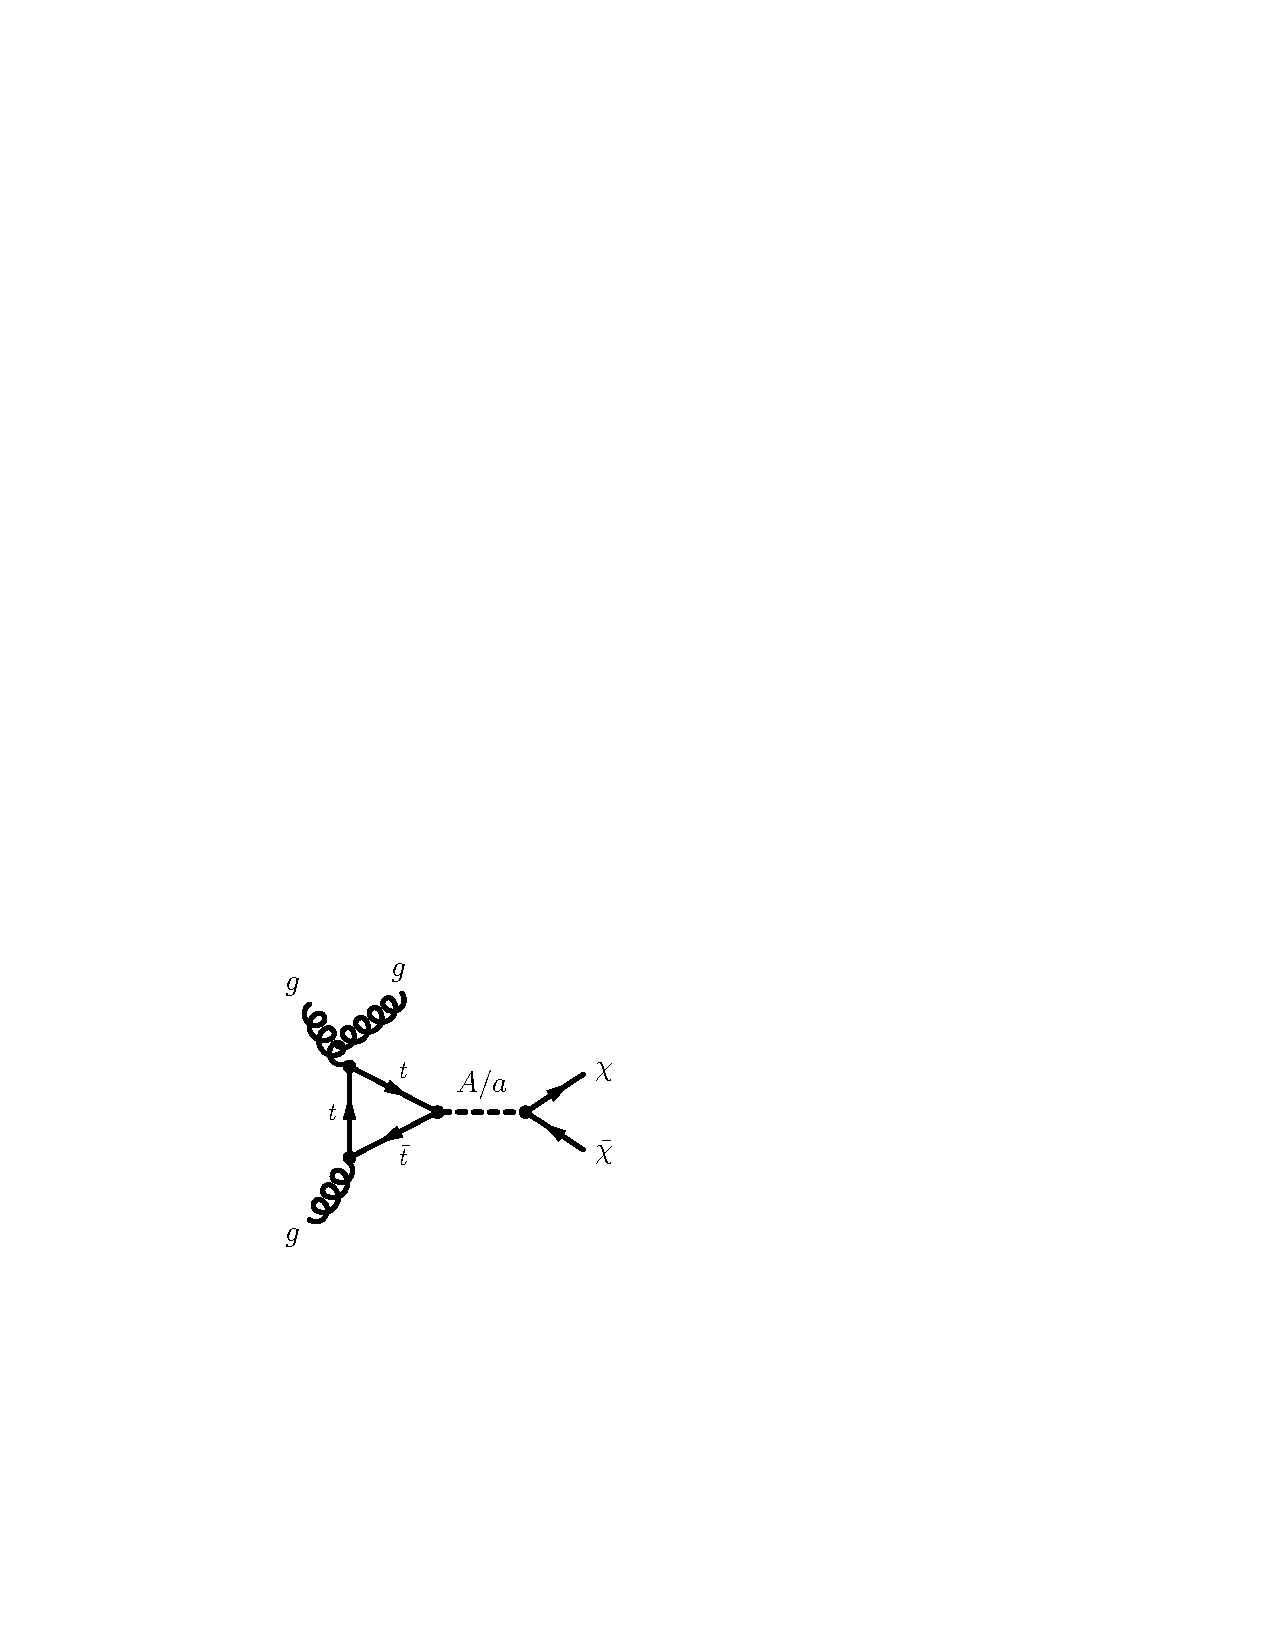
\includegraphics[width=0.6\textwidth]{figures/fig_01c.pdf}
        \vfill
        \caption{Gluon-gluon fusion}
        \label{subfig:metj-gg-fusion}
    \end{subfigure}
    \hfill
    \begin{subfigure}[3]{0.48\textwidth}
        \centering
        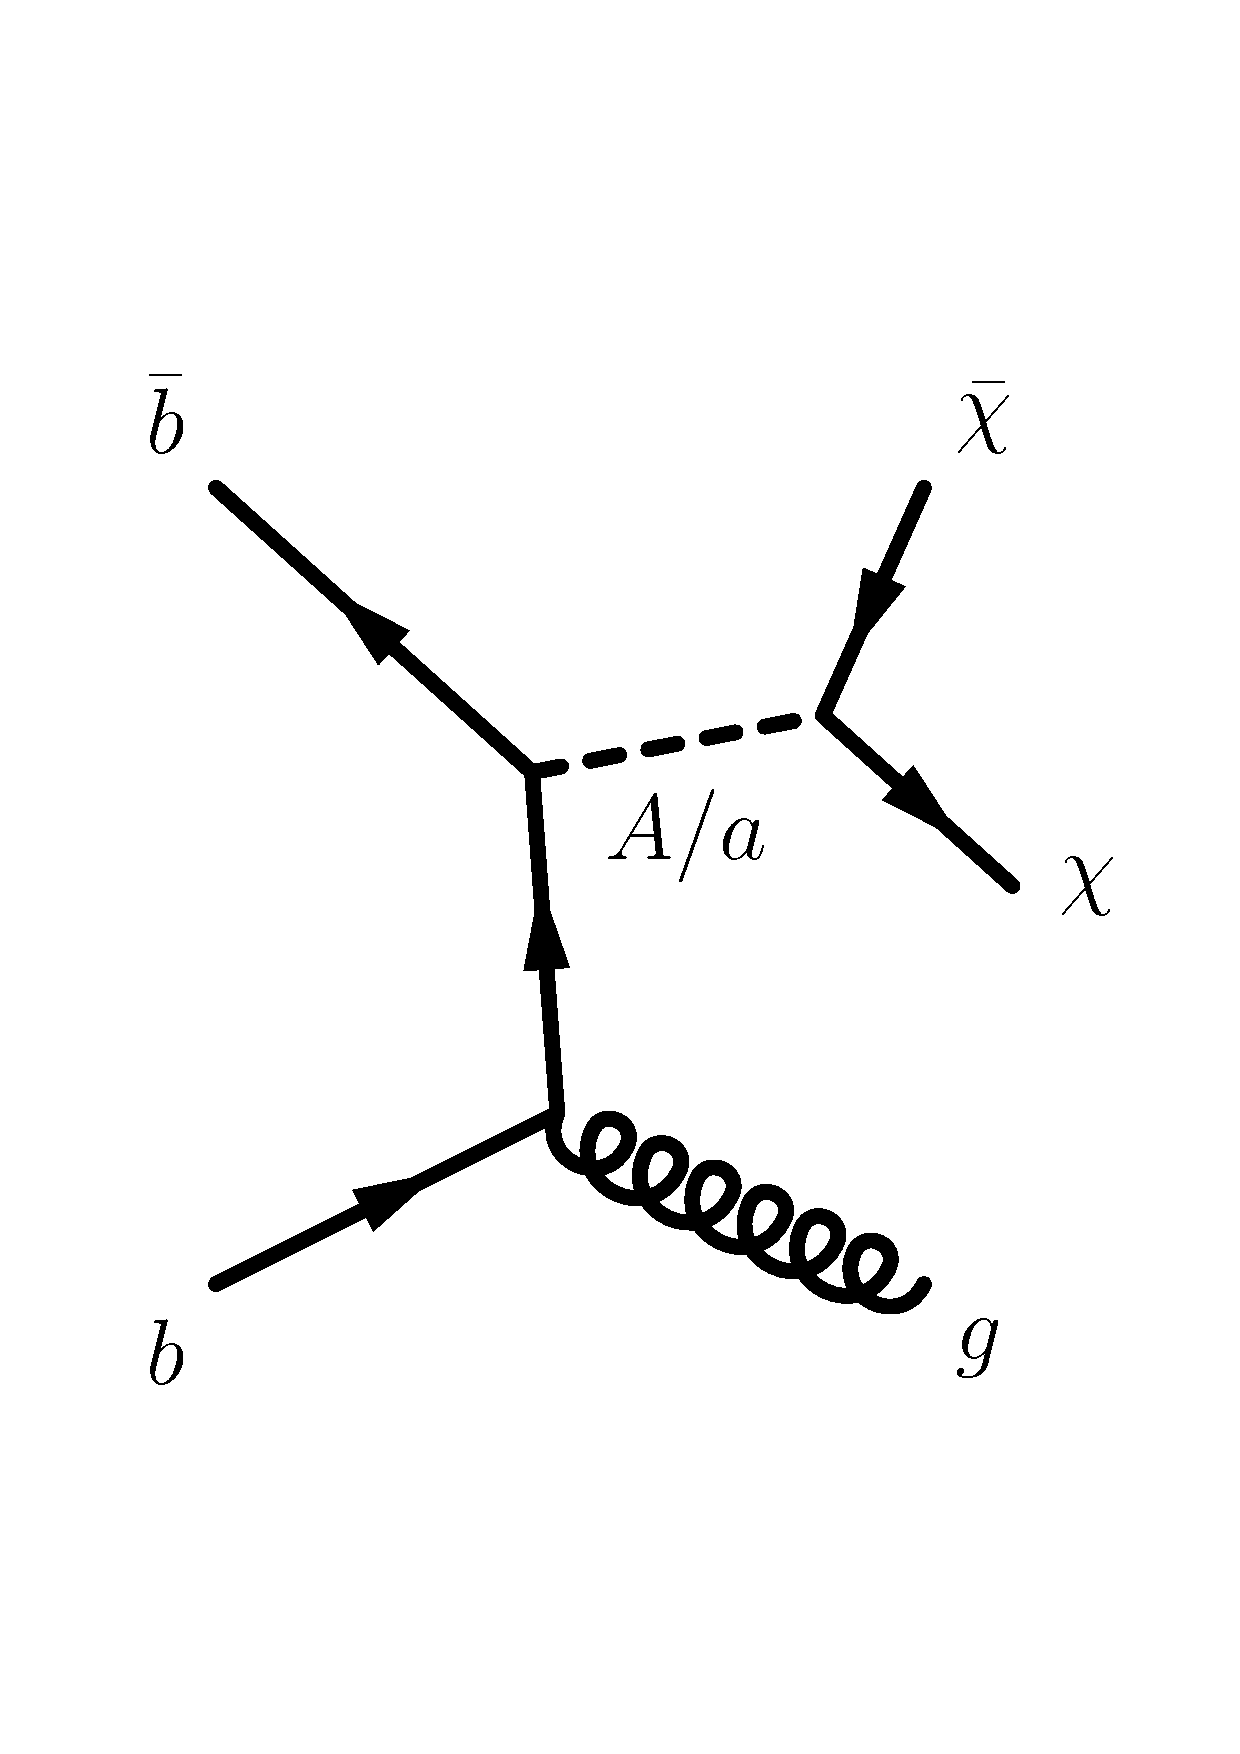
\includegraphics[width=0.6\textwidth]{figures/fig_02e.pdf}
        \caption{$b\bar{b}$-initiated}
        \label{subfig:metj-bb-associated}
    \end{subfigure}
    \caption{Production mechanisms and final state of the $\met+j$ signature, including gluon-gluon fusion production (a) and $b\bar{b}$-initiated production (b).}
    \label{fig:metj-signature}
\end{figure} 

This search targets final states containing a single jet and a large $\met$, which must satisfy $\met>200$ GeV to guarantee full $\met$ trigger efficiency for all selected events \cite{EXOT-2018-06}. Events must contain a leading jet with $p_T>150$ GeV, $\abs{\eta} < 2.4$, up to three additional jets with $p_T>30$ GeV, $\abs{\eta} < 2.8$, and no leptons or photons. The azimuthal angular separation between the $\met$ vector and each jet is required to meet $\Delta\phi(\met, jet) > 0.6$ for events with $200 < \met < 250$ GeV, and $\Delta\phi(\met, jet) > 0.4$ for those with $\met > 250$ GeV to reduce multijet backgrounds. 

Dominant SM backgrounds include $Z(\nu\nu)$ and $W(l\nu)$ production, in which the $W$ decays into a $\tau$-lepton which later decays hadronically, or other leptons that are undetected. Other contributions arise from $t\bar{t}$, single top quark, and diboson production, as well as non-collision and multijet backgrounds. These background contributions are estimated using a profile likelihood fit to the $p_T$ distribution of the system recoiling against the reconstructed jets in both signal and control regions.

In this combination, the search is reinterpreted in the context of \hdma, which is not considered in the original search. Several signal contributions to this signature are considered. In the low-$\met$ region, the production of a pair of DM particles with a jet is the primary contribution at $\met< 500$ GeV $m_a\le 150$ GeV. Both $gg$-initiated and $bb$-initiated productions are considered, the latter of which is relevant at large $\tanb$. For larger $\met$ and smaller $m_a$, the production of two pairs of DM particles via $h\rightarrow aa \rightarrow \chi\bar{\chi}\chi\bar{\chi}$ (figure \ref{fig:haaff-signature}) is the dominant process. Smaller contributions come from $\met+Z(q\bar{q})$ and $\met + h(b\bar{b})$ productions which the invisible decays of the SM Higgs boson are kinematically forbidden. Finally, minor contributions from $pp\rightarrow t\bar{t} +a$, and $pp\rightarrow tW+a$ are also present.

\subsection{\texorpdfstring{$\hinv$}{TEXT} signature}

The invisible decays of the SM Higgs boson represented by a $\met$ associated to other visible signatures have been investigated in previous ATLAS publications and statistically combined in Ref \cite{HIGG-2021-05}. The main production mechanisms include vector-boson fusion (VBF) \cite{EXOT-2020-11}, VBF with an emitted photon \cite{EXOT-2021-17}, gluon-gluon fusion \cite{EXOT-2018-06}, associated production with a vector boson \cite{HIGG-2018-26}, and associated production with a pair of top quarks \cite{SUSY-2019-12}. The results from Run 2 searches are combined statistically with constraints on invisible Higgs decays obtained from searches with up to 4.7 $\ifb$ of $pp$ collision data at $\sqrt{s}=7$ TeV and 20.3 $\ifb$ at $\sqrt{s}=8$ TeV \cite{HIGG-2015-03}. 

Among these searches, $\hinv$ from VBF production from Run 2 is the most sensitive and sets an observed limit of 0.145 and an expected limit of 0.103 at $95\%$ confidence level on the invisible branching ratio. Selected events are required to pass the $\met$ trigger and have $\met>160$ GeV. They must also contain from two to four jets with $p_T>25$ GeV, among which the leading and sub-leading jets must have $p_T^{lead}>80$ GeV and $p_T^{sub-lead}>50$ GeV and be well separated in $\eta$. In addition, lepton and $b$-jet vetoes are applied to reduce $W+jets$ and top quark backgrounds. By partitioning the $\met$ spectrum, the jet multiplicity, and jet-invariant masses, sixteen orthogonal signal regions are defined. Dominant background processes include $Z(\nu\nu)+jet$ and $W(l\nu)+jet$ production, the latter of which the charged lepton is undetected or misidentified. The backgrounds are estimated from control regions in the one-lepton and two-lepton channels. The multijet background is directly estimated from data. An upper limit on the $\hinv$ of $0.113\left(0.080^{+0.031}_{-0.022} \right)$ is observed (expected) at $95\%$ confidence level. 

\subsection{Additional searches using 36 \texorpdfstring{\ifb}{TEXT} of \texorpdfstring{$\sqrt{s}=13$}{TEXT} TeV \texorpdfstring{$pp$}{TEXT} collision data}

Three searches using 36 $\ifb$ of $\sqrt{s}=13$ TeV data are shown in this combination, the first of which targets $\met + Z(q\bar{q})$ signature \cite{EXOT-2016-23}. The final state contains a $\met>150$ GeV and a hadronically decaying vector boson reconstructed as a single large-$R$ jet with $p_T>250$ GeV in a boosted topology and two small-$R$ jets with $p_T>20$ GeV in a resolved topology. A lepton veto is applied in both cases. Signal regions are defined using the number of $b$-jets in the final state. The dominant backgrounds of $t\bar{t}$ and $W/Z+jets$ are estimated using a simultaneous fit to the $\met$ distribution in he signal and control regions.

The second search targets a $\met+b\bar{b}$ signature. The final state contains at least two $b$-jets and $\met>180$ GeV \cite{SUSY-2016-18}. The irreducible background from $Z(\nu\nu)+b\bar{b}$ events separated from the signal events using the azimuthal separation between the $b$-jets and the $\met$. The results are extracted from a likelihood fit to the angular observable $\cos\theta*_{b\bar{b}} = \abs{\tanh\Delta\eta_{n\bar{b}}/2}$, in which $\Delta\eta_{n\bar{b}}$ is the difference in pseudorapidity between the $b$-jets.

The last group of searches targeting $\met+t\bar{t}$ and differing the the number of final-state leptons are included \cite{SUSY-2016-18}. A search in the final state where both $W$ boson decay hadronically selects events with at least four energetic jets, of which at least two are $b$-jets, and a large $\met$. Several requirements on the invariant mass of the large-$R$ jets are applied to identify events with a boosted $W$ boson or top quark decay. The main backgrounds are $Z+jets$, $t\bar{t}$, and $t\bar{t}+Z$ production, constrained using dedicated control regions. A search in the one-lepton final state, resulting from a leptonically decaying $W$ boson, selects events with at least four energetic jets, at least one of which is a $b$-jet, an isolated lepton, and a large $\met$ \cite{SUSY-2016-16}. They must also have at least a hadronic top candidate with invariant mass close to the top quark mass. The azimuthal separation between the lepton and $\met$ and that between the jets and $\met$ are used to suppress the background contamination in the signal regions. Dedicated control regions are used to estimate background processes involving top quarks.

\subsection{\texorpdfstring{$\htb$}{TEXT} signature}
\label{subsect:tbHtb}
The leading-order Feynman diagram for the target signature of this search is shown in figure \ref{fig:tbHtb-signature} \cite{HDBS-2018-51}. The charged Higgs boson is produced together with a top and a bottom quark, and subsequently decays into a top and a bottom quark, in which one top quark decays semi-leptonically. Events are preselected to contain exactly one electron or muon with $p_T>27$ GeV at at least five jets with $p_T>25$ GeV. At least three jets must be $b$-tagged to reduce large backgrounds from multijet production. Selected events are divided into four separate regions, namely $5j3b$, $5j\ge 4b$, $\ge 6j3b$, and $\ge 6j\ge 4b$, where $j$ and $b$ respectively stand for jets and $b$-jets. A neural network is trained to discriminate between signal and background, whose output distributions are used to extract the signal in data. 

Dominant backgrounds include $t\bar{t}+jets$, and single top quark production in the $Wt$ channel. The former is divided into $t\bar{t}+\mathrm{light}$, $t\bar{t}+\ge 1b$, and $t\bar{t}+\ge 1c$. These along with other minor backgrounds are model using MC simulation and corrections obtained from an additional $\ge 5j2b$ region via a reweighting procedure \cite{ATL-PHYS-PUB-2018-009, TOPQ-2018-18}. After the reweighting, the $t\bar{t}+\ge 1b$ and $t\bar{t}+ \ge 1c$ normalizations factors are extracted from the fit to data. 

\begin{figure}[h!]
    \centering
    \begin{subfigure}[3]{0.48\textwidth}
        \centering
        \begin{tikzpicture}
          \begin{feynman}
            \vertex (h) at (0,0);
            \vertex (tgp) at (-0.3, 1) ;
            \vertex (bgp) at (-0.3, -1) ;
            \vertex (gt) at (-1.8, 1.2) {$g$};
            \vertex (gb) at (-1.8, -1.2) {$g$};
            \vertex (t) at (1.4, 1.2) {$t$} ;
            \vertex (b) at (1.4, -1.2) {$\bar{b}$};
            \vertex (htb) at (1.2, 0) ;
            \vertex (th) at (2.1, 0.6) {$\bar{t}$};
            \vertex (bh) at (2.1, -0.6) {$b$};
            \diagram[] {
                (h) -- [fermion] (tgp),
                (bgp) -- [fermion] (h),
                (gt) -- [gluon] (tgp),
                (gb) -- [gluon] (bgp),
                (tgp) -- [fermion] (t),
                (b) -- [fermion] (bgp),
                (h) -- [scalar, edge label=\(H^{-}\)] (htb),
                (htb) -- [anti fermion] (th),
                (bh) -- [anti fermion] (htb),
            };
          \end{feynman}
        \end{tikzpicture}
    \end{subfigure}
    \caption{Production mechanisms and final state of the $\htb$ signature.}
    \label{fig:tbHtb-signature}
\end{figure} 

\subsection{\texorpdfstring{$t\bar{t}t\bar{t}$}{TEXT} signature}

\begin{figure}[h!]
    \centering
    \begin{subfigure}[3]{0.48\textwidth}
        \centering
        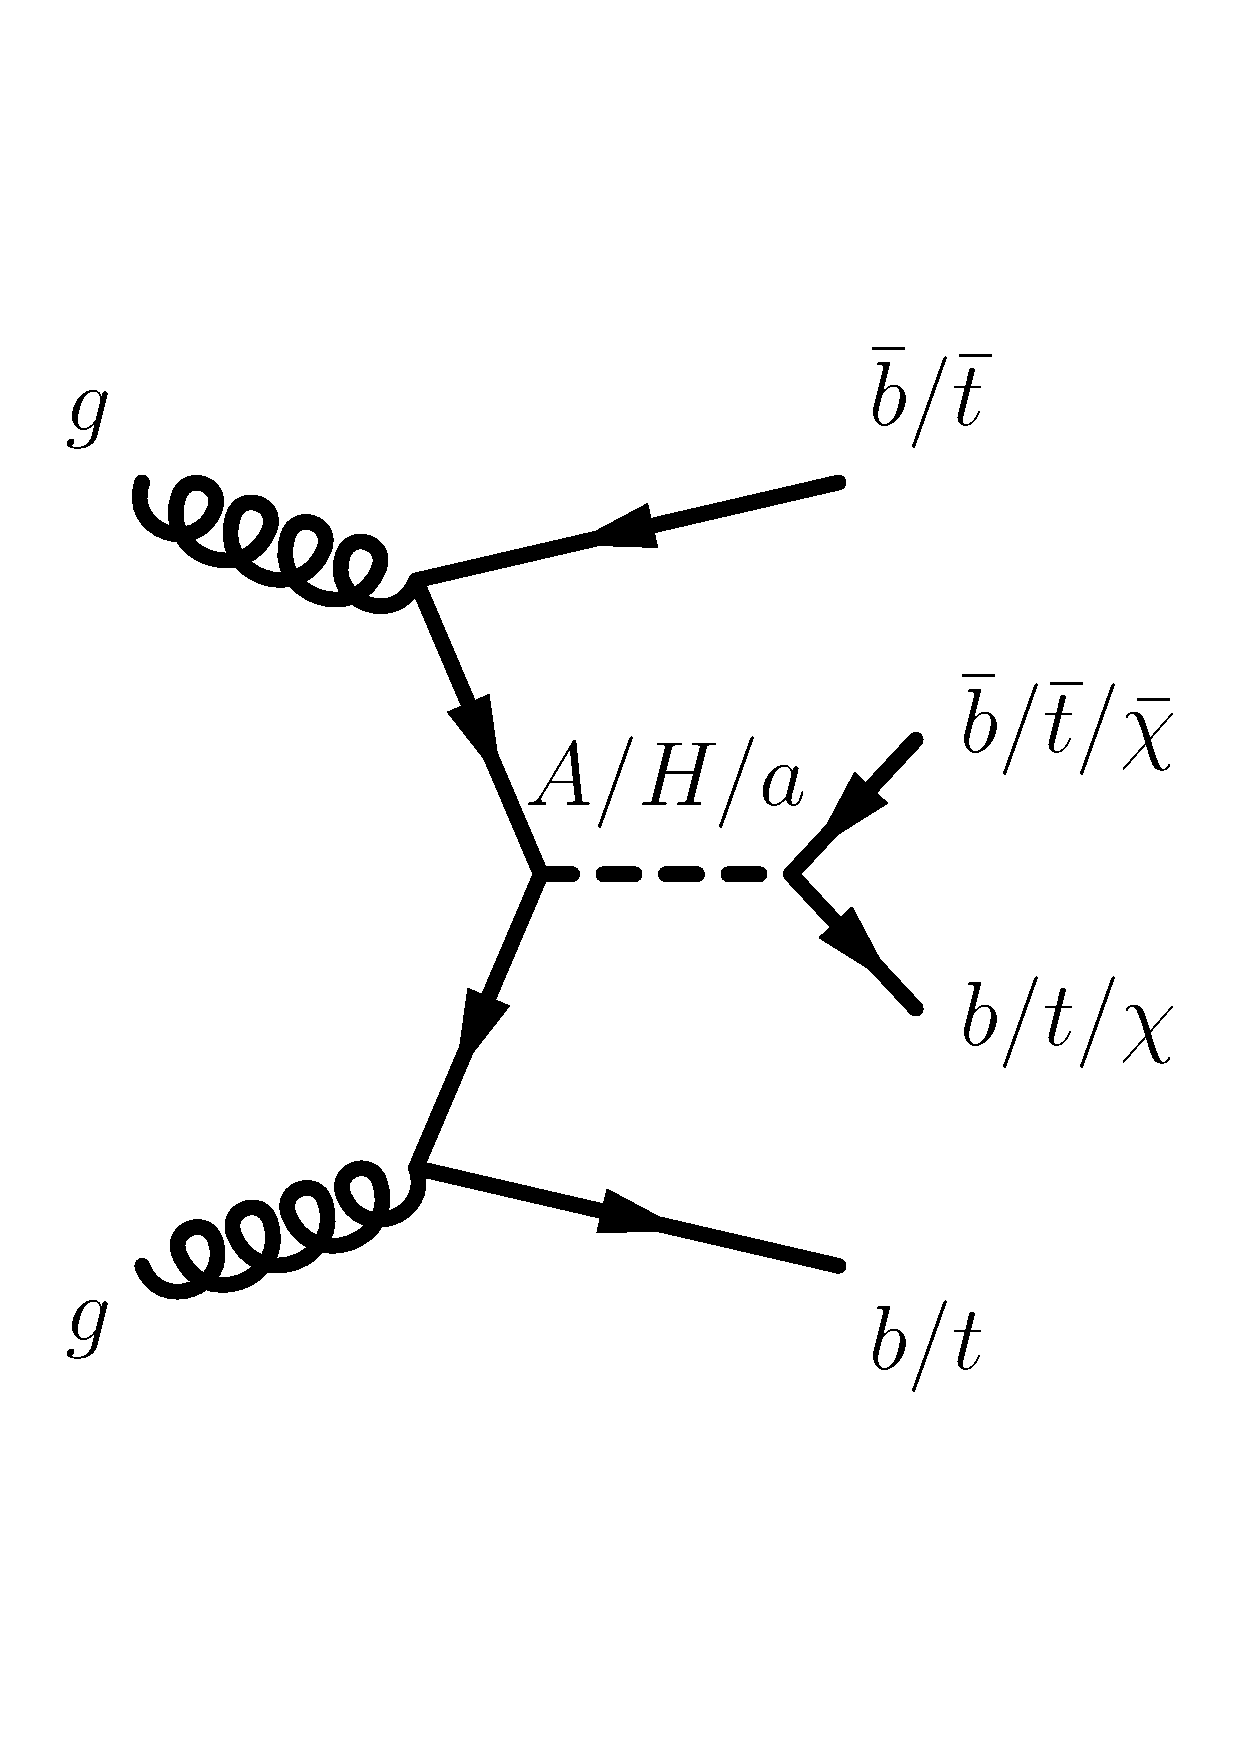
\includegraphics[width=0.7\textwidth]{figures/fig_01e.pdf}
    \end{subfigure}
    \caption{Production mechanisms and final state of the $t\bar{t}t\bar{t}$, $\met+b\bar{b}$, and $\met+t\bar{t}$ signatures.}
    \label{fig:tttt-signature}
\end{figure} 

The targeted signature of this search, shown in figure \ref{fig:tttt-signature}, is a $t\bar{t}$-associated production of a heavy scalar or pseudo-scalar Higgs boson in the \hdma, which then decays into a pair of top quarks\cite{EXOT-2019-26}. The final state contains 2 pairs of top quarks, decaying into either two leptons with the same-sign electric charge or at least three leptons, both with high jet multiplicity. These leptons include electrons or muons from leptonic $\tau$ decay, and are required to have $p_T>28$ GeV. A baseline signal region is defined by requiring six jets with $p_T>25$ GeV, among which at least two are $b$-tagged, and a scalar sum of the all transverse momenta of jets and leptons $H_T>500$ GeV. First, a BDT is trained to separate SM $t\bar{t}t\bar{t}$ production and background processes using event-level inputs. A second BDT, designated BSM mass-parametrised BDT (BSM pBDT), is then trained to discriminate between BSM $t\bar{t}t\bar{t}$ events and all background. It is parametrised as a function of the mass of the heavy Higgs boson by introducing the mass as an input in the training \cite{Baldi:2016fzo}.

The major irreducible backgrounds arise from the top quark pair production with a boson and jets ($t\bar{t}+W+jets$, $t\bar{t}+Z+jets$, and $t\bar{t}+h+jets$). These contributions are estimated using MC simulations with data-driven corrections for $t\bar{t}+W+jets$. Minor, irreducible backgrounds originate mostly from $t\bar{t}+jets$ and $tW+jets$ production with mis-identified charge, fake and non-prompt leptons, which are estimated from data using dedicated control regions.

\subsection{Exotic Higgs boson decays \texorpdfstring{$h\rightarrow aa\rightarrow f\bar{f}f'\bar{f}'$}{TEXT}}

\begin{figure}[h!]
    \centering
    \begin{subfigure}[3]{0.48\textwidth}
        \centering
        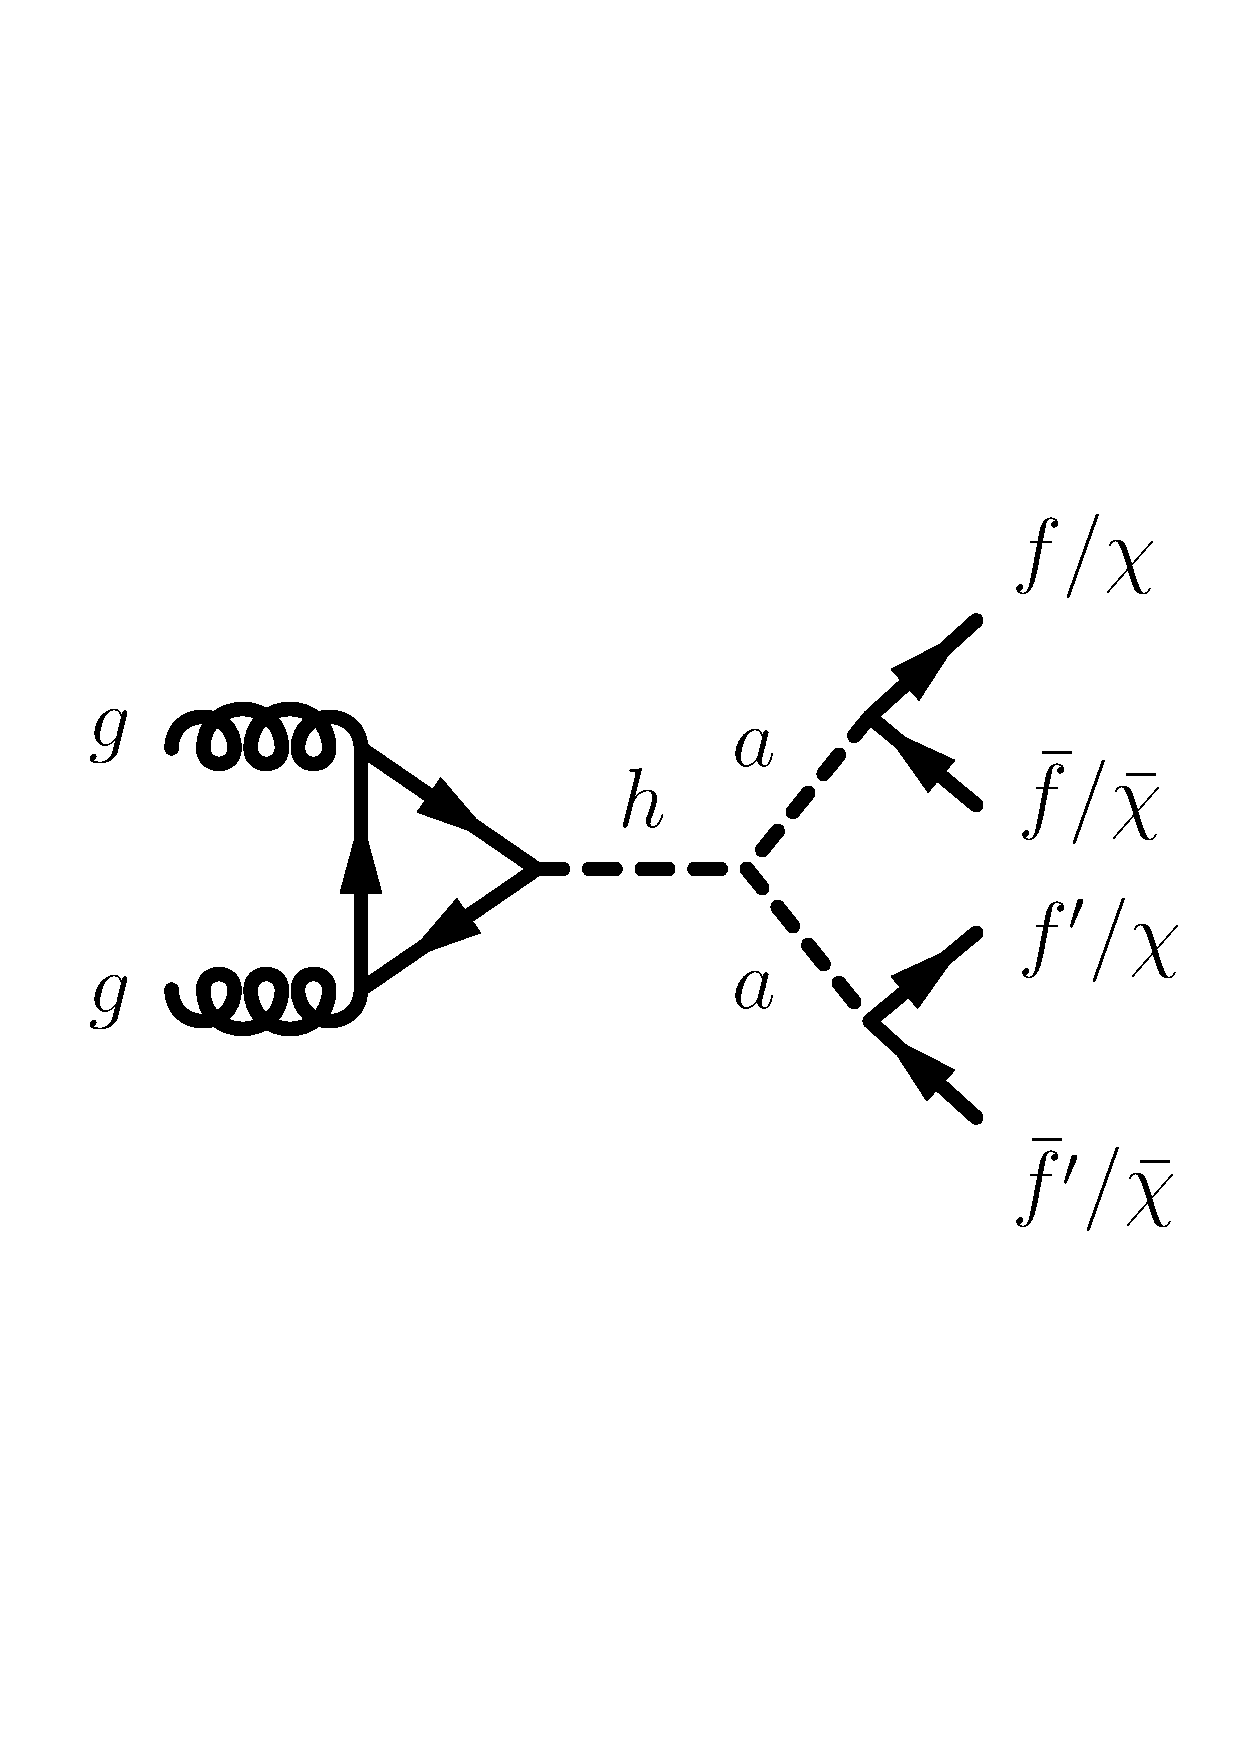
\includegraphics[width=0.7\textwidth]{figures/fig_01g.pdf}
    \end{subfigure}
    \caption{Production mechanisms and final state of the $h\rightarrow aa\rightarrow f\bar{f}f'\bar{f}'$ signature.}
    \label{fig:haaff-signature}
\end{figure} 

This set of searches target the decays of the SM Higgs boson into a pair of light pseudo-scalar particles $aa$, which then decay into four fermions, as illustrated in figure \ref{fig:haaff-signature}. Depending on the type of fermion present in the final state, the searches provide sensitivity to different pseudo-scalar mass ranges.

The first search uses 139 $\ifb$ of $\sqrt{s}=13$ TeV $pp$ collision data, and targets the $b\bar{b}\mu^+\mu^-$ final state \cite{HDBS-2021-03}. It is sensitive to pseudo-scalar mass in the range $16<m_a<62$ GeV. The variable of interest is the dimuon invariant mass, chosen to probe for a resonant enhancement over the SM expectation. The dominant background is the Drell-Yan dimuon process together with $b$ quarks and SM $t\bar{t}$ production where both $W$ bosons from the top quarks decay into a muon and a neutrino. 

A second search using 36 $gn^{-1}$ of $\sqrt{s}=13$ TeV $pp$ collision data targeting $b\bar{b}b\bar{b}$ final state provides sensitivity in the mass range $20<m_a<60$ GeV \cite{HIGG-2017-05}. The Higgs boson is produced in associated with a leptonically decaying $W$ boson (one-lepton channel) or $Z$ boson (two-lepton channel). Signal-background separation is performed with a BDT trained using event-level kinematic variables, notably the reconstructed pseudo-scalar masses. The dominant background process in the one-lepton channel is $t\bar{t}$ production with additional jets, and $Z+jet$ in the two-lepton channel. The BDT output distribution is used as the observable of interest in the final likelihood fit. This search is optimized for the resolved topology of the $b\bar{b}$ dijet system, i.e. they are reconstructed as two small-$R$ jets. 

A third search on 20.3 $\ifb$ of $\sqrt{s}=8$ TeV $pp$ collision targeting $\mu^+\mu^-\tau^+\tau^-$ probes the mass range $3.7<m_a<50$ GeV. It probes resonant enhancement in the dimuon invariant mass spectrum \cite{HIGG-2014-02}.

The last searches considered in this combination target final states with four charged leptons ($l=e,\,\mu)$) on 36 $\ifb$ and 139 $\ifb$ of $\sqrt{s}=13$ TeV \cite{EXOT-2016-22, HDBS-2018-55}. They each probes two orthogonal pseudo-scalar mass regions, namely a low-mass region covering $1<m_a<15$ GeV range, excluding the mass ranges around the $J/\psi$ and the $\Upsilon$ resonances, and a high-mass region covering $15<m_a<60$ GeV. The high-mass range is insensitive to \thdma and therefore excluded from this combination. The final states containing at least four muons are exclusively considered thanks to their large branching ratio and the large selection efficiency of isolated muons relative to that of isolated electrons. The dominant background process is $ZZ^*\rightarrow \mu^+\mu^-\mu^+\mu^-$ and $h\rightarrow ZZ^*\rightarrow \mu^+\mu^-\mu^+\mu^-$. The observable of interest is the average dimuon invariant mass $\expval{m_{\mu^+\mu^-}} = (m_{12} + m_{34})/2$, in which the pairing is done to minimize the dimuon invariant mass difference. 

Model-independent upper limit on the branching ratio of the $h\rightarrow aa \rightarrow 4f$ are obtained. The upper limit is used directly to exclude parameter regions in the \thdma based on the predicted $h\rightarrow aa \rightarrow 4f$ branching ratio for each point considered in the benchmark scenarios in the previous section. 


\section{Systematic uncertainties}
\label{sect:systematic-uncertainties}

Systematic and statistical uncertainties depend on event selection, the considered phase space, and the background estimation strategy. Systematic uncertainties may be of experimental or theoretical origin. In general, experimental uncertainties may uncertainties in the absolute jet energy scales and resolutions, jet quality requirements, pile-up corrections, $b$-jet identification efficiencies, and the soft contributions to $\met$. Uncertainties in lepton identification and reconstruction efficiencies, energy/momentum scale and resolution are considered fro events with selected or vetoed leptons. Uncertainties due to the finite size of the background MC samples and others related to the modelling of the background processes are also included in the analyses. A luminosity uncertainty of 1.7\% is applied to backgrounds derived purely from MC simulation \cite{ATLAS-CONF-2019-021}. 

Theoretical uncertainties on the production cross-section or on the signal acceptance affect signal modelling. They include uncertainties related to the PDF and are evaluated following the PDF4LHC recommendations \cite{Butterworth:2015oua}. Other uncertainties pertain to the choice of renormalization and factorization scales. They are derived by varying independently such scales by a factor of 2.0 and 0.5 relative to the nominal values used for MC generation. In addition, for signatures entering the statistical combination, uncertainties in the modelling of initial- and final-state radiation and multi-parton interactions are taken into account. 

\section{Statistical combination of results}
\label{sect:stat}
Three \thdma signatures are selected to enter a statistical combination, namely $\monohbb$, $\monozll$, and $tbH^{\pm}tb$. They cover complementary regions of the model parameter space, and are the most constraining signatures of those described in \ref{sect:exp-signatures}. These factors simplify the statistical treatment and enhance the sensitivity to the \thdma signal.

These input analyses are statistically independent, due to their event selection. The $\monozll$ analysis vetoes events with $b$-jets, whereas the other analyses require the presence of at least two jets. The $tbH^{\pm}tb$ targets final states with a charged lepton, while $\monohbb$ vetoes the presence thereof. Therefore, the signal region of these analyses are completely separated. A small event overlap ($<1\%$) is observed between $\htb$ signal region and the leptonic control region of the $\monohbb$ analysis, but has no impact on the combination.

\subsection{Statistical analysis}

To statistically combine the results of these analyses, a combined likelihood function is constructed and the corresponding profile likelihood ratio maximized \cite{Cowan:2010js}. The common parameter of interest (POI) is the signal strength of a \thdma signal at a particular point in the parameter space, defined as the ratio of the observed number of signal event to the signal cross-section times branching ratio. Systematic uncertainties are introduced to the likelihood as constrained nuisance parameters (NPs), denoted by $\theta_{\mu}$, and modelled by Gaussian, Poisson, or Log-normal probability density function. Background normalization factors, denoted by $\lambda_{\mu}$, are floated without constraints in the fit to estimate the background components in their corresponding control regions. 

The combined likelihood is given by
\begin{equation}
    \label{4.13}
    L(\mathrm{data}|\mu,\lambda_{\mu},\theta_{\mu})= \prod_{c=1}^{N_c} {L}_c(\mathrm{data}|\mu, \lambda_{\mu}, \theta_{\mu}) \prod_{k=1}^{N_{cons}} {F}(\Tilde{\theta}_{\mu, k}|\theta_{\mu, k}),
\end{equation}
where $N_c$ is the number of categories, $c$ the index of the event category, $N_{cons}$ the number of constrained NPs, $k$ the index of the NP, $\Tilde{\theta}_{\mu, k}$ the global observable corresponding to $\theta_k$, and $F$ the constraining probability distribution function corresponding to the type of uncertainty. 

The $95\%$ confidence level (CL) limits are obtained by the CLs frequentist formalism \cite{ReadCLs} using the profile likelihood ratio test statistics ($q_{\mu}$)\cite{Cowan:2010js}, defined as 
\begin{equation}
    \label{4.14}
    q_{\mu} = \begin{cases} 
     -2\ln\frac{L(\mathrm{data}|\mu,\hat{\hat{\lambda}}_{\mu},\hat{\hat{\theta}}_{\mu})}{L(\mathrm{data}|0,\hat{\hat{\lambda}}_{0},\hat{\hat{\theta}}_{0})}\quad &  \hat{\mu}<0, \\
        -2\ln\frac{L(\mathrm{data}|\mu,\hat{\hat{\lambda}}_{\mu},\hat{\hat{\theta}}_{\mu})}{L(\mathrm{data}|\hat{\mu},\hat{\lambda}_{\mu},\hat{\theta}_{\mu})}\quad & 0\le \hat{\mu}<\mu, \\
        0 \quad & \hat{\mu} > \mu
    \end{cases}
\end{equation}
where the numerator is the likelihood maximized for a given fixed value of $\mu$, and the denominator is the globally maximized likelihood. The single-hat quantities denote the global optimum values, while the double-hat quantities denote the optima at $\mu$, i.e. a function of $\mu$.
% The confidence level is determined from the $p$-values of the $b$-only hypothesis and the different $s+b$ hypotheses,
% \beq
% \label{chap:phys-ana:15}
% \mathrm{CL}_s = \frac{p_{s+b}}{1-p_{b}}.
% \eeq
% Each signal hypothesis corresponds to a particular point in the parameter space.
% The $p$-value of the null hypothesis $p_b$ and the signal hypothesis is obtained by setting $q_0=0$ and evaluating $q_1$ in equation \eqref{4.14} respectively and integrating over the corresponding sampling distribution \cite{Cowan:2010js}.
% A signal model, i.e. a parameter point, is said to be excluded at $95\%$ CL when $CL_s<0.05$. 


\subsection{Uncertainties and their correlations}

Each of the three analyses treats a particular set of uncertainties. Often times, more than one analysis estimate the same systematic uncertainty, in which case it is correlated. This section describes this treatment. Most experimental uncertainties are correlated across search channels, namely they are modelled using the same observable in the combined likelihood. They include uncertainties related to the reconstruction of physics objects, the integrated luminosity, and pile-up modelling. Physics object uncertainties include those from electrons, muons, and the jet energy response. Uncertainties from $b$-jet identification depend on $b$-tagging algorithm and working point, which vary across the analyses. As a result, they are not correlated. Finally, several experimental systematic uncertainties are moderately constrained in a particular analysis, and hence not correlated to avoid phase-space biases. Different assumptions on the correlation of uncertainties related to jet, $\met$, and $b$-jet identification, and other moderately constrained uncertainties are tested to gauge their impact on the observed exclusions, and found to have negligible impact. 

Uncertainties on signal simulation and background modelling are assessed for each analysis. To each final state is dedicated a separate signal simulation, as they often probe different kinematic regions of the phase space. The theoretical uncertainties are found to be small and are considered to be uncorrelated. Uncertainties pertaining to background modelling are considered correlated amongst the analyses, motivated by their different sources of leading background, different probed kinematic phase space, as well as different methods of background estimation.

\subsection{The impact of uncertainties}

Different \thdma parameter values correspond to different signal kinematics and sensitivity delivered by each analysis, and thus see different levels of impact from uncertainties on the combined signal strength. As an example, the contributions to the uncertainty of the best fit signal strength from statistical and systematic uncertainties are shown in table \ref{tab:uncertainty-contribution} for a parameter point at $m_a=450$ GeV, $m_H=800$ GeV, $\tanb=1.0$, and $\sint=0.35$. This signal is not excluded by any single input analysis, but is excluded by the combination. The statistical uncertainty is slightly smaller than the systematic counterpart, which is broken into three categories: theoretical, experimental, and MC statistical uncertainties. The impact of each category is estimated by fixing the uncertainties in that category in a fit, and subtracting the resulting uncertainty in the signal strength from the total in quadrature. Theoretical uncertainties arise mainly from uncertainties in background modelling and are slight smaller than experimental ones. Among the experimental uncertainties originating from reconstructed physics objects, those from jet and $\met$ make the largest contributions. 

For each input analysis, the most important uncertainties also make the largest contribution to the combined uncertainty. For background modelling, the largest components are $ZZ$ modelling from $\monozll$, $t\bar{t}$ uncertainties from $\met+h(bb)$, and uncertainties from $t\bar{t}$ production with additional $b$ quarks from $\htb$. Among experimental systematic uncertainties, the largest sources are lepton systematic uncertainties from $\monozll$, uncertainties related to jets and $\met$ from $\met+h(bb)$, and those related to $b$-jet identification from $\htb$.

\begin{table}
    \centering
    \begin{tabular}{lllr}
    \hline\hline
        \multicolumn{3}{l}{Uncertainty source} & $\Delta\mu\cdot 100$\\
        \hline
        \multicolumn{3}{l}{Statistical uncertainty}  & $25.0$ \\
        \hline
         \multicolumn{3}{l}{Systematic uncertainty}  & $27.6$ \\
         &  \multicolumn{2}{l}{Theory uncertainties}  &  $16.2$\\
         & & Signal modelling & $2.8$ \\
         & & Background modelling & $15.9$ \\
         & \multicolumn{2}{l}{Experimental uncertainties (excl. MC stat.)} & $18.8$ \\
         & & Luminosity, pile-up & $3.9$ \\ 
         & & Jets, $\met$ & $12.3$ \\
         & & Identification of $b$-jets & $9.1$ \\
         & & Electrons, muons & $6.1$ \\
         & \multicolumn{2}{l}{MC statistical uncertainty} & $9.3$ \\
         \hline
         \multicolumn{3}{l}{Total uncertainty} & $37.2$ \\
    \hline\hline
    \end{tabular}
    \caption{Impact from different sources of uncertainties on the best-fit signal strength express in $\Delta\mu$ on the signal at $(m_A=800\, \mathrm{GeV}, m_a=450 \, \mathrm{GeV}, \tanb=1, \sint=0.35)$, estimated by fixing the corresponding NPs to their best-fit values, and subtracting the resulting uncertainty from the total uncertainty in quadrature. The statistical uncertainty component is obtained by fixing all NPs except the floating background normalization factors, and quantifies the impact of the limit data yields in the signal and control regions. The total uncertainty is not the quadratic sum of the individual contribution due to correlations between systematic uncertainties }
    \label{tab:uncertainty-contribution}
\end{table}

\section{Results on combined constraints on the \thdma}

A summary of combined constraints on \thdma across all benchmark scenarios introduced in section \ref{sect:benchmark-scenarios} is presented in this section. 

\subsection{Scenario 1: \texorpdfstring{$m_a-m_A$}{TEXT} planes}
Figure \ref{fig:result-ma-mA-scan} shows the exclusion contours from the $m_a-m_A$ scans with the 2HDM mixing angle fixed to $\sint=0.35$ in \ref{fig:result-ma-mA-scan-a} and \ref{fig:result-ma-mA-scan-c}, and $\sint=0.7$ in \ref{fig:result-ma-mA-scan-b} and \ref{fig:result-ma-mA-scan-d}. These choices of parameters correspond to benchmark scenarios 1a and 1b in section \ref{sect:benchmark-scenarios}. The combined exclusion contours are shown along with those of the three individual channels entering the statistical combination in \ref{fig:result-ma-mA-scan-a} and \ref{fig:result-ma-mA-scan-b}, and with the remaining channels in \ref{fig:result-ma-mA-scan-b} and \ref{fig:result-ma-mA-scan-d}. Over the two benchmark parameter planes, the $\monozll$ and $\monohbb$ drive the sensitivity across a large region, due primarily to the resonant production of the scalar and pseudo-scalar according to the diagram in figures \ref{subfig:zll-gg-fusion-res} and \ref{subfig:hbb-gg-fusion-res}. Their sensitivity varies widely with the pseudo-scalar Higgs boson and the mediator masses. At $\sint=0.35$ and in the region where $\monozll$ and $\monohbb$ dominate, all pseudo-scalar mass is excluded up to a maximum $m_a=560$ GeV for $m_A=1.2$ TeV, while for $m_a=1.5$ GeV, all pseudo-scalar Higgs mass is excluded up to $m_A=1.55$ TeV. At $\sint=0.7$, all pseudo-scalar mass is excluded up to a maximum $m_a=550$ GeV for $m_A=1$ TeV, while for $m_a=400$ GeV, all pseudo-scalar Higgs mass is excluded up to $m_A=1.2$ TeV. For both choices of $\sint$, the $\monozll$ contour reaches closer to the $m_A=m_a$ limit than that of $\monohbb$, because the former can probe lower $\met$ values, whereas the latter is sensitive at higher $\met$ due to the presence of a $\met$ trigger in its selection and the mass difference between the $Z$ and the Higgs bosons. In addition, the exclusion power of $\monohbb$ is increased relative to $\monozll$ at high $m_A$ and low $m_a$, because of an increase in the cross-section of the non-resonant $a^*\rightarrow ah$ process, without resonant $A$ production, which has no equivalence in the latter's signature.

\begin{figure}[h!]
    \centering
    \begin{subfigure}[2]{0.495\textwidth}
        \centering
        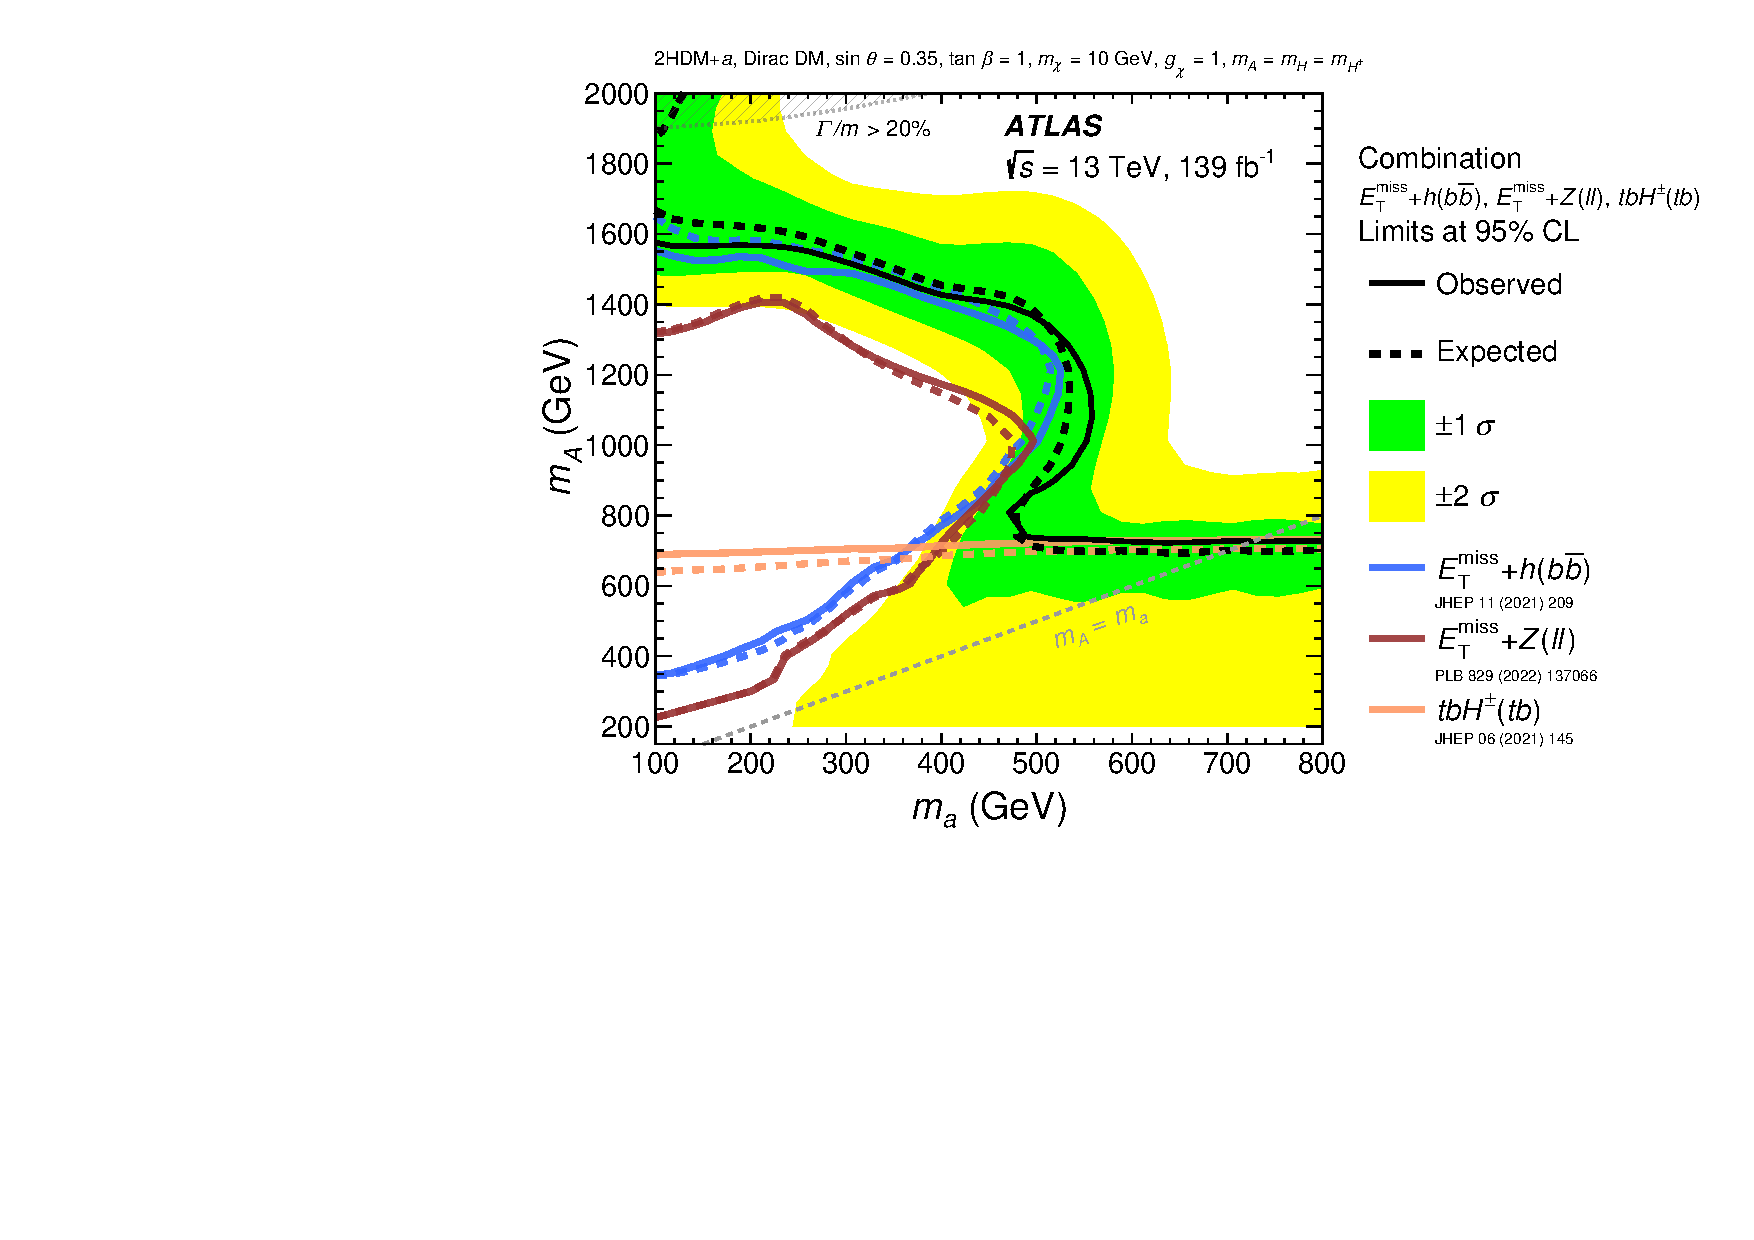
\includegraphics[width=\linewidth]{figures/fig_04a.pdf}
        \caption{}
        \label{fig:result-ma-mA-scan-a}
    \end{subfigure}
    \begin{subfigure}[2]{0.495\textwidth}
        \centering
        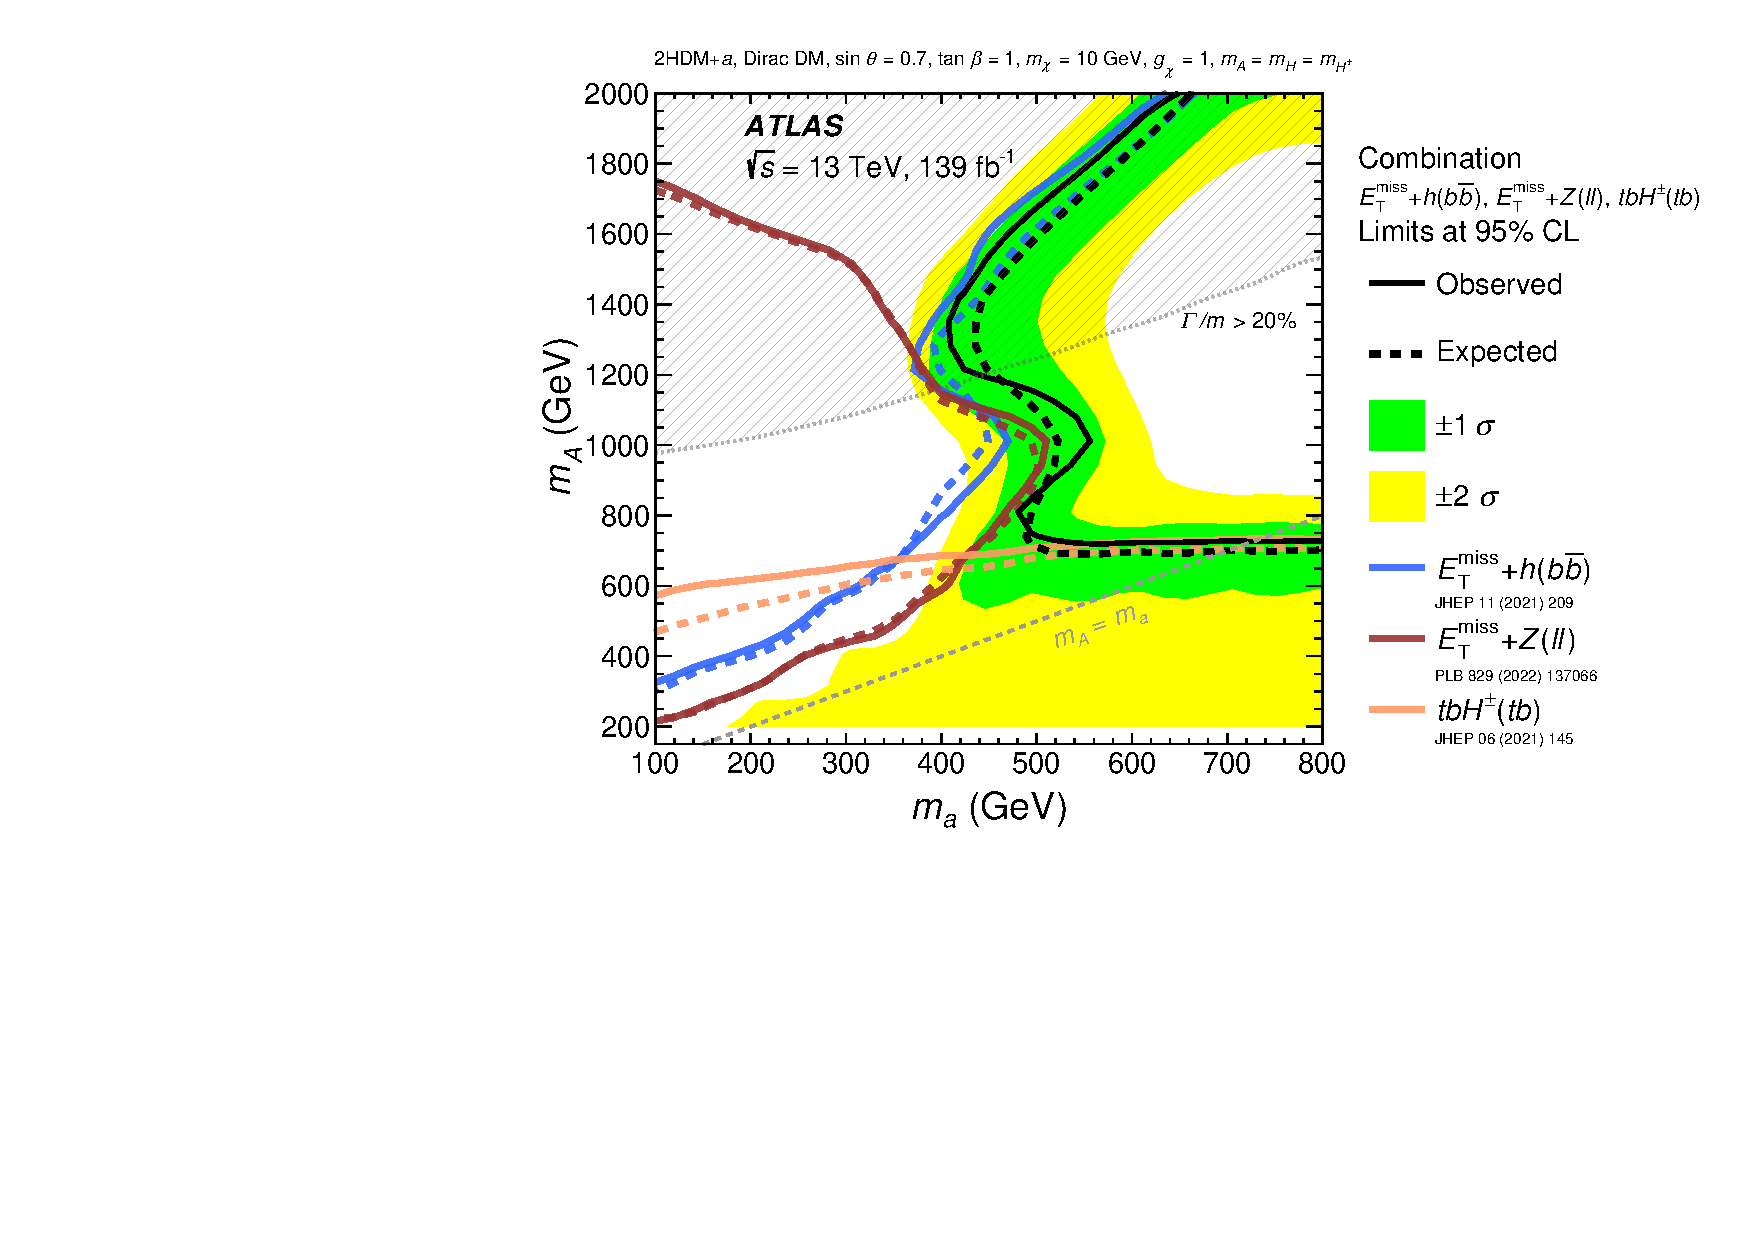
\includegraphics[width=\linewidth]{figures/fig_04b.pdf}
        \caption{}
        \label{fig:result-ma-mA-scan-b}
    \end{subfigure}
    \begin{subfigure}[2]{0.495\textwidth}
        \centering
        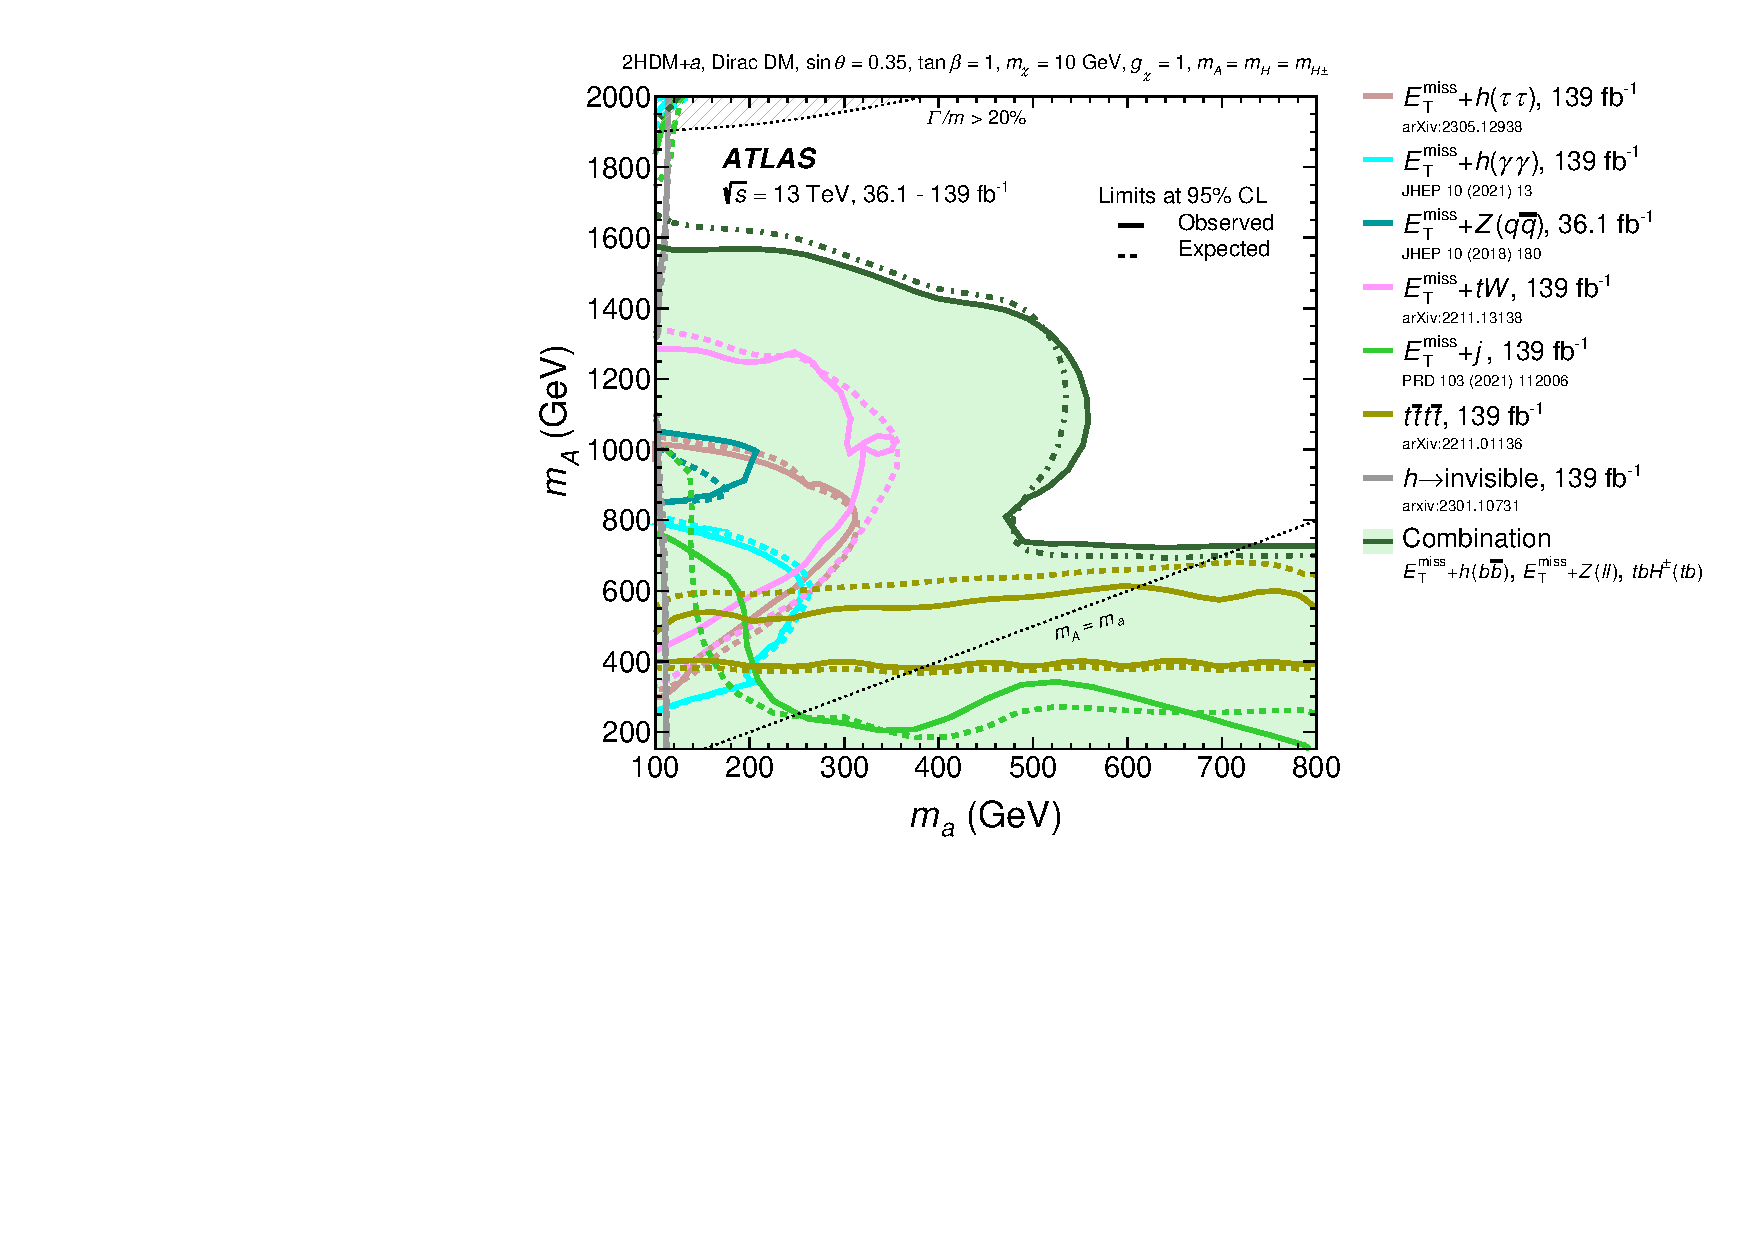
\includegraphics[width=\linewidth]{figures/fig_04c.pdf}
        \caption{}
        \label{fig:result-ma-mA-scan-c}
    \end{subfigure}
    \begin{subfigure}[2]{0.495\textwidth}
        \centering
        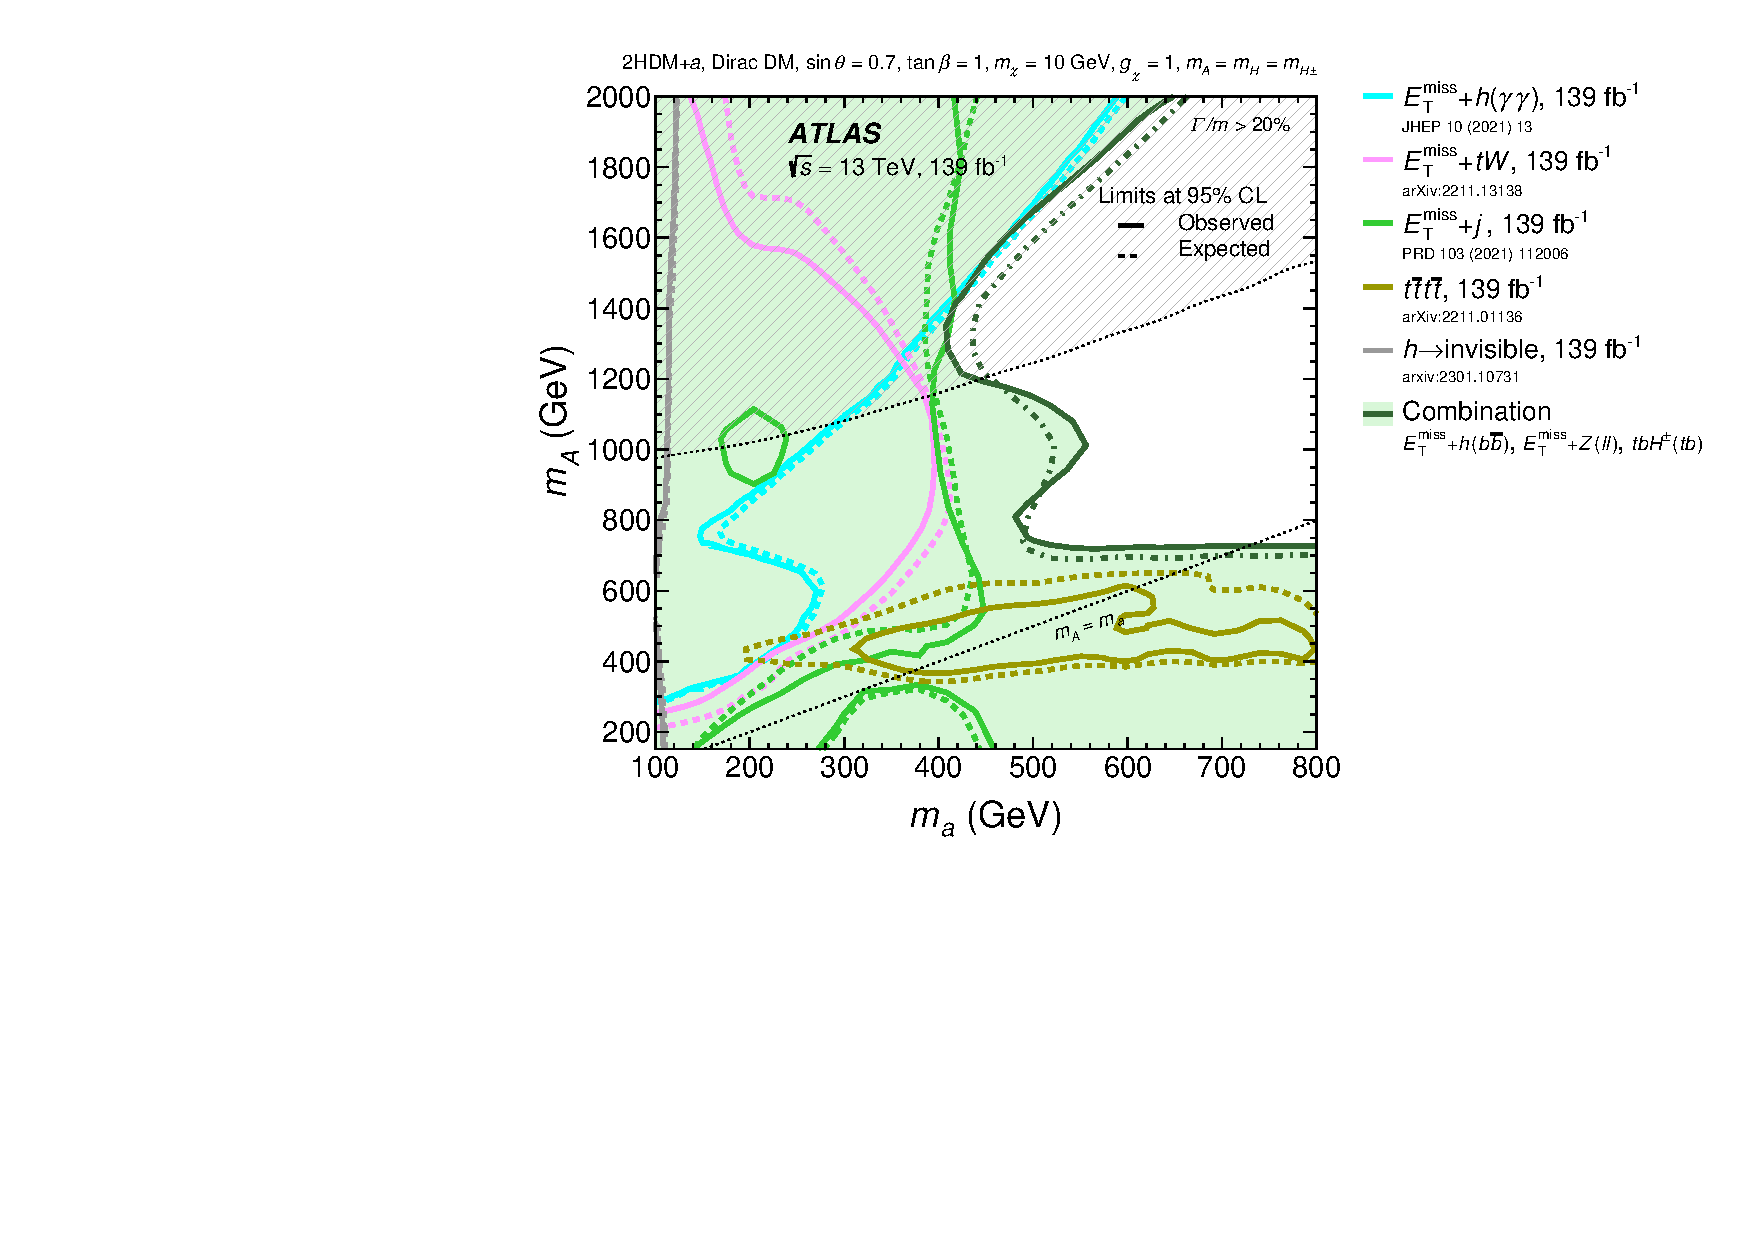
\includegraphics[width=\linewidth]{figures/fig_04d.pdf}
        \caption{}
        \label{fig:result-ma-mA-scan-d}
    \end{subfigure}
    \caption{Observed and expected exclusion regions at $95\%$ CL over the $(m_a, m_A)$ plane evaluated at \thdma mixing angles $\sint=0.35$ (subfigures (a), (c)), and $\sint=0.7$ (subfigures (b), (d)). The observed and expected contours are respectively shown in solid and dashed lines in all subsequent figures. In (a) and (b), the observed and expected exclusion limits from each of the three statistically combined signatures are shown along with the combined limits. The green and yellow shared bands respectively correspond to the $\pm1$ and $\pm2$ standard deviation uncertainty in the combined expected limits. In (c) and (d), the combined exclusion contours are overlaid along those of additional channels not included in the statistical combination. In all subfigures, a dashed grey region indicates the region where the width of any of the Higgs boson exceeds $20\%$ of its mass. }
    \label{fig:result-ma-mA-scan}
\end{figure} 

For both values of $\sint$, the $\htb$ channel excludes complementary regions where the other channels provide less exclusion power. For $\sint=0.35$ all pseudo-scalar Higgs masses up to $m_A\le 700$ GeV are excluded, and for $\sint=0.7$, the upper bound of the excluded $m_A$ ranges from 600 GeV to 700 GeV. The weak dependence on the mediator mass $m_a$ is due to the absence of the mediator in its signature, such that its sensitivity is only indirectly affected by $m_a$ via the competition from other possible decay modes, for instance $H^{\pm}\rightarrow aW^{\pm}$. This the reduction in branching ratio is observed at $\sint=0.7$, where the limits from this channel weakens at lower $m_a$, where the aforementioned decay is kinematically possible. The statistical combination with $\htb$ augments the excluded parameter space above $m_a=500$ GeV and below $m_A=700$ GeV for both scenarios. 

The exclusion power of other channels not entering the statistical combination varies widely and demonstrated on figures \ref{fig:result-ma-mA-scan-c} and \ref{fig:result-ma-mA-scan-d}. The \monohgamgam search probes a region in the parameter space that is similar in shape to that of the $\monohbb$ search, only smaller due to the smaller branching ratio of the $h\rightarrow \gamma\gamma$ decay relative to the $h\rightarrow b\bar{b}$ decay. At lower values of $m_A$ however, it becomes more sensitive than $\monohbb$, as it does not rely on the $\met$ trigger and is capable of probing smaller values of $\met$, similar to the better sensitivity of $\monozll$ relative to $\monohbb$ in the same region. Similar to the $\monohbb$ search, the \monohgamgam shows a significant boost in sensitivity at higher $m_A$ for $\sint=0.7$, due to an increase in the cross-section of the $a\rightarrow ah$ process. 

The $h\rightarrow \tau\tau$ search is only interpreted at $\sint = 0.35$, and its exclusion contour has a similar shape to that of other $\met+h$ signatures, but is even smaller in coverage due to a small branching ratio relative to the $h\rightarrow b\bar{b}$ final state. 

The exclusion contours of the $\met+tW$ search have a similar shape to those of the $\monozll$ search for both values of $\sint$, albeit smaller in exclusion area. The observed exclusion consistently covers a smaller area of the phase space than the expected sensitivity, due to a small excess in the $2$-lepton channel of less than $2\sigma$ significance \cite{EXOT-2018-43}. 

The sensitivity of the $\met+j$ search shows interesting features on the $m_a-m_A$ plane. The signature does not contain resonant production as in the case of the $Z/h$ boson in figures \ref{subfig:zll-gg-fusion-res} and \ref{subfig:hbb-gg-fusion-res}. Therefore, the exclusion contour differ significantly from the $\met+Z$ and $\met+h$ signatures. In addition, the signal cross-section is affected by the inference between non-resonant contributions from the pseudo-scalars $a$ and $A$, which depends on both $m_a$ and $m_A$, especially at the larger value of the mixing angle $\sint$ \cite{Bauer:2017ota}. A small difference in pseudo-scalar mass $(m_a\approx m_A)$ leads to destructive interference, reducing the signal cross-section and thus the sensitivity to the \hdma. This effect is observed for both values of $\sint$. At $\sint=0.35$, the $\met+j$ search excludes values of $m_a$ up to 600 GeV for $m_A\approx 200$ GeV, and values of $m_A$ up to 800 GeV for $m_a\approx 100 $ GeV. At $\sint=0.7$, stronger mixing leads to higher cross-sections for signal hypotheses with $m_A>m_a$. For $m_A\approx 1300$ GeV, all values of $m_a$ up to $\approx 400$ GeV are excluded, comparable to the exclusion power of the $\monozll$ and $\monohbb$ searches. 

The $t\bar{t}t\bar{t}$ search is sensitive in regions where the $\monozll$ and $\monohbb$ searches have lower sensitivity, similar to the $\htb$ search. However, unlike the latter, it is only sensitive to the \thdma when either of the pseudo-scalar masses is above the production threshold of a top quark pair $(m_{A/a}\ge 2m_t)$. For $\sint = 0.35$, the contour is almost independent of $m_a$, driven largely by the resonant production of the heavy Higgs bosons $A/H$. For $\sint = 0.7$, the sensitivity is lowered for small $m_a$ compared to the scenario with $\sint=0.35$ due to a larger $a-A$ and a forbidden $a\rightarrow t\bar{t}$ decay.

The exclusion contours from the $\met + Z(q\bar{q})$ search on 36 $\ifb$ data are shown for scenario 1a \cite{EXOT-2017-32}. The search provides the smallest sensitivity because it suffers from larger multijet production backgrounds and smaller data sample.

\subsection{Scenario 2: \texorpdfstring{$m_A-\tanb$}{TEXT} planes}

Figure \ref{fig:result-mA-tanb-scan} summarizes the exclusion limits over the $m_A-\tanb$ parameter plane evaluated with $\sint = 0.35$ and $\sint = 0.7$. In both scenarios, a large portion of the parameter plane is excluded by the combined contours. At $\sint=0.35$ the combined sensitivity is driven primarily by the $\monozll$ search, which is also observed at lower pseudo-scalar mass at $\sint=0.7$. At higher values of $m_A$, the $\monohbb$ provides stronger constraints. In general, the sensitivity of these channels is influence by the transition from $gg$- to $bb$-initiated production of the $Z/h$ boson, and finds its minimum in the region around $\tanb=5$. 

\begin{figure}[h!]
    \centering
    \begin{subfigure}[2]{0.495\textwidth}
        \centering
        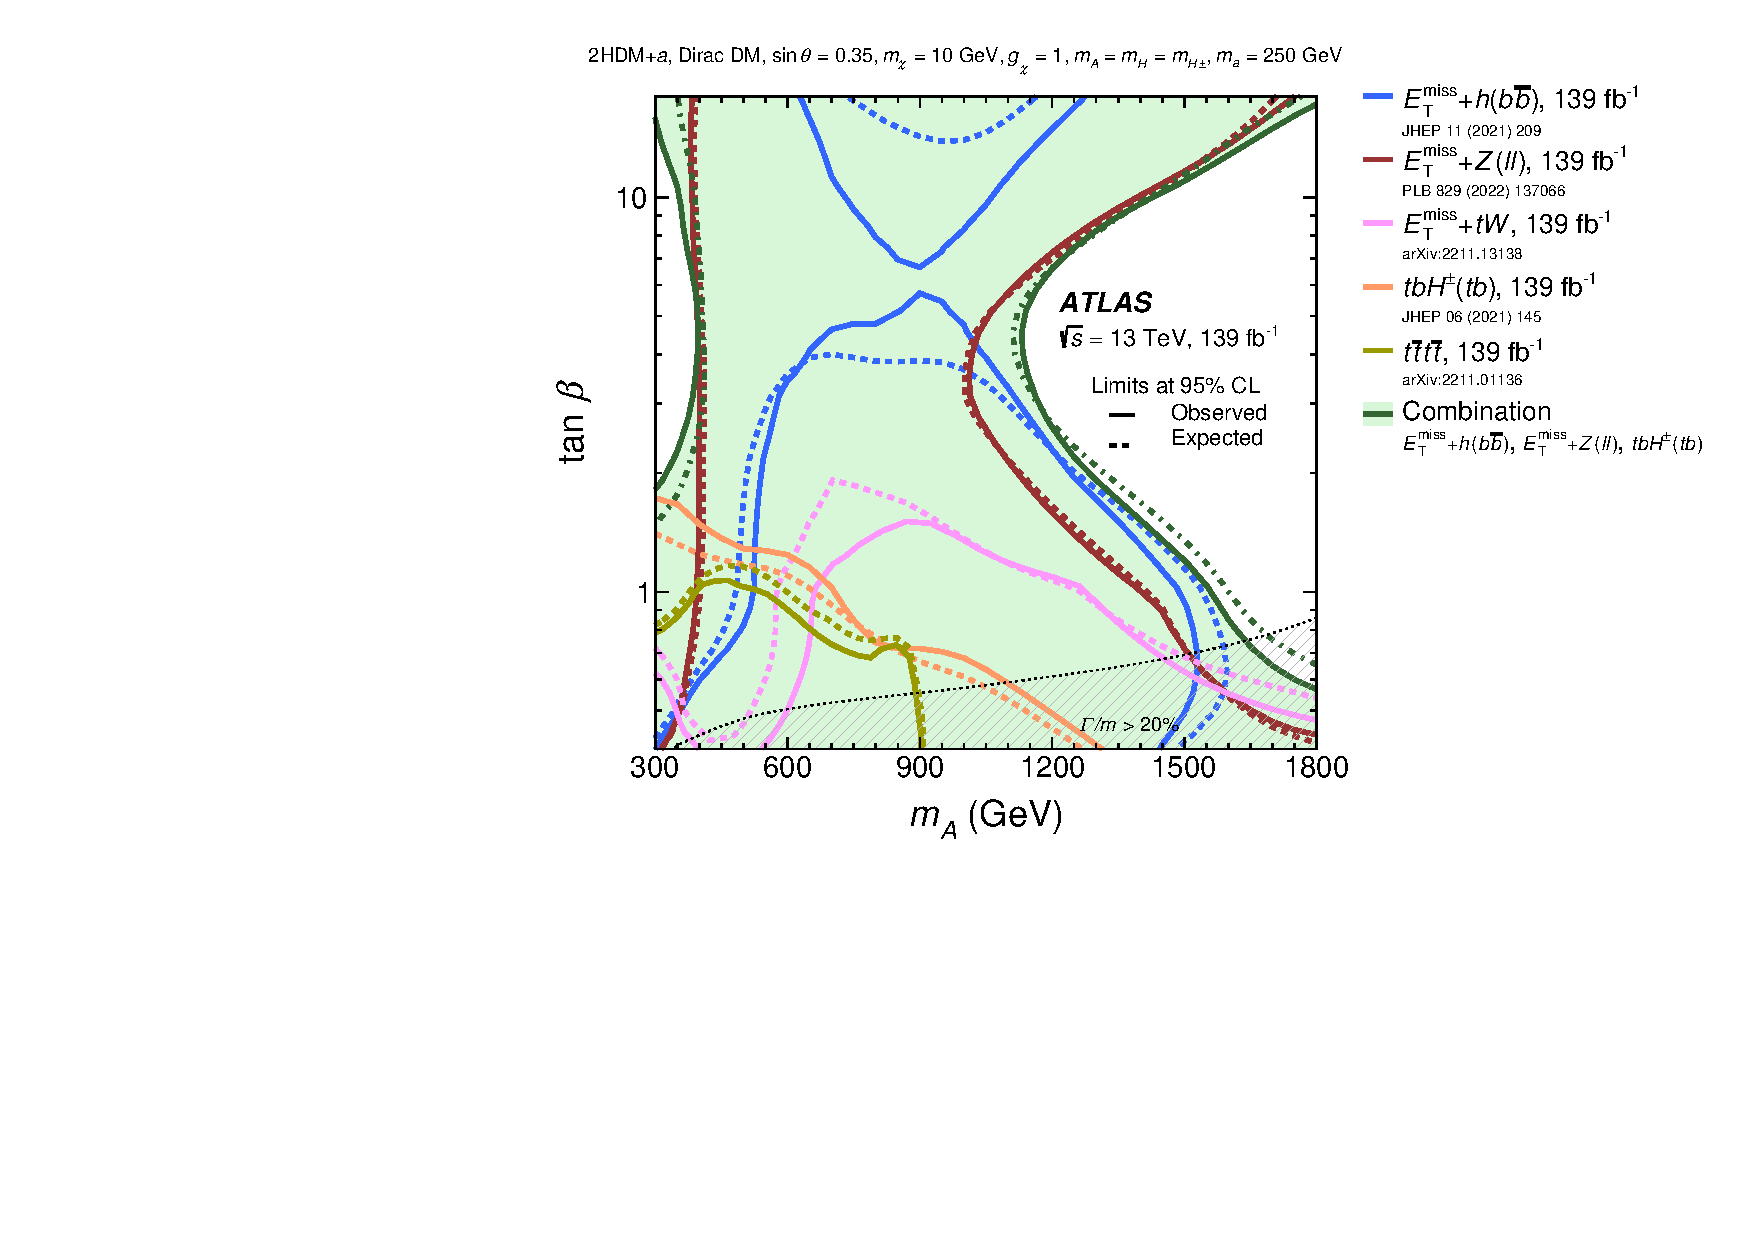
\includegraphics[width=\linewidth]{figures/fig_05a.pdf}
        \caption{}
        \label{fig:result-mA-tanb-scan-a}
    \end{subfigure}
    \begin{subfigure}[2]{0.495\textwidth}
        \centering
        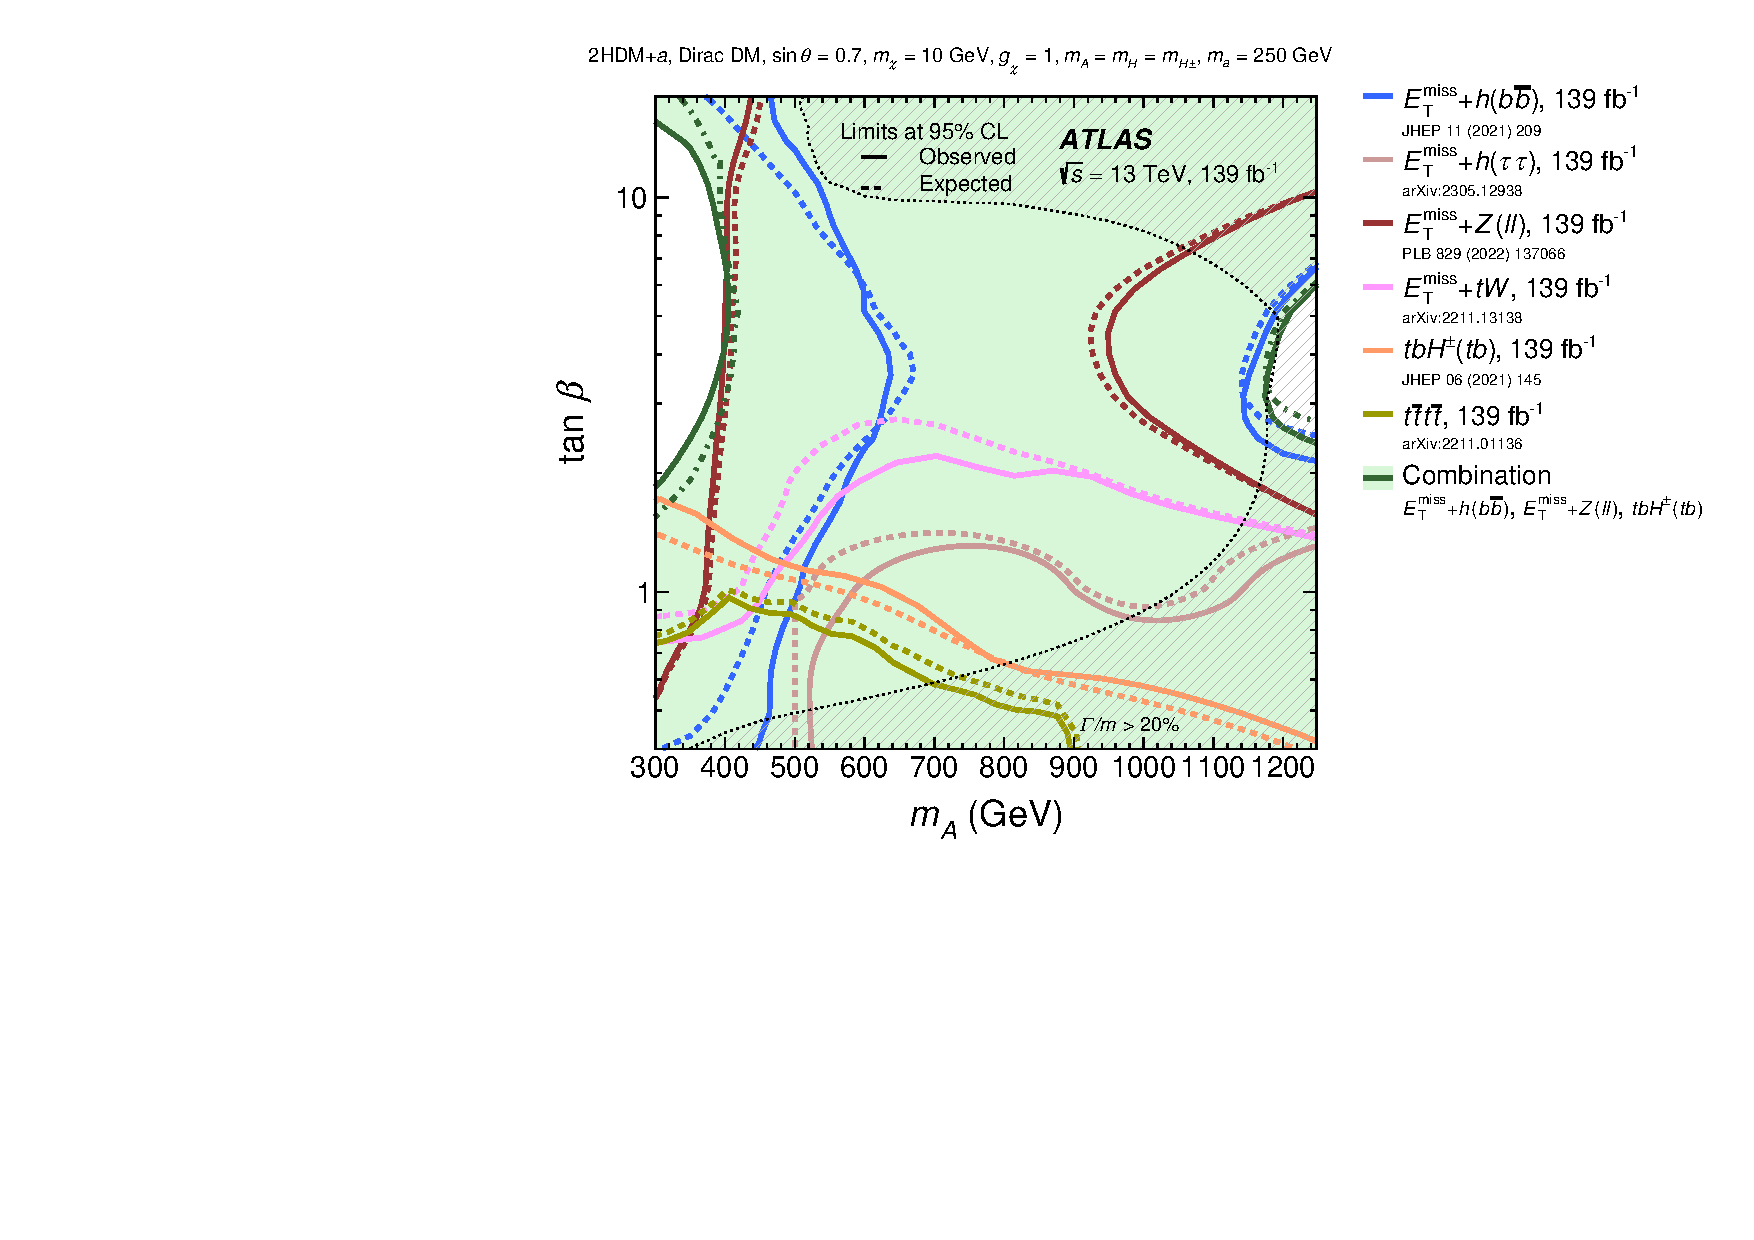
\includegraphics[width=\linewidth]{figures/fig_05b.pdf}
        \caption{}
        \label{fig:result-mA-tanb-scan-b}
    \end{subfigure}
    \caption{Observed and expected exclusion regions at $95\%$ CL over the $(m_A, \tanb)$ plane evaluated at \thdma mixing angles $\sint=0.35$ (a), and $\sint=0.7$ (b). The statistical combined contours are shown along with those from individual searches. In both subfigures, a dashed grey region indicates the region where the width of any of the Higgs boson exceeds $20\%$ of its mass. }
    \label{fig:result-mA-tanb-scan}
\end{figure} 

The $\met+tW$ search excludes regions of the parameter space up to $\tanb=1.5$ for $\sint=0.35$ and $\tanb=2$ for $\sint=0.7$. The observed sensitivity in both scenarios is weaker than the expected counterpart because of a small excess in the two-lepton signal region of the search \cite{EXOT-2018-43}. The larger mixing angle again shows better sensitivity to the $\met+tW$ signature \cite{Pani:2017qyd}. 

The exclusion contour from the $\met+h(\tau\tau)$ search is evaluated as a function of $m_A$ and $\tanb$ only at $\sint=0.7$. Because of the small branching ratio of the $h\rightarrow \tau\tau$ decay, it has low sensitivity for the \thdma signal. 

The $t\bar{t}t\bar{t}$ and $\htb$ searches provide sensitivity at low values of $m_A$ and $\tanb$, due to enhanced production cross-section for smaller resonance masses and a preference for coupling to third generation quarks in this region.

\subsection{Scenario 3: \texorpdfstring{$m_a-\tanb$}{TEXT} planes}

Figure \ref{fig:result-ma-tanb-scan} summarizes the exclusion limits as a function of the $m_a$ and $\tanb$ evaluated at $\sint = 0.35$ (scenario 3a) and $\sint = 0.7$ (scenario 3b). In both scenarios, the $\monozll$ search drives the sensitivity over a large portion of the parameter plane. The $\monohbb$ and \monohgamgam searches exclude analogous regions, albeit the latter covers a smaller area, due to the smaller $h\rightarrow \gamma\gamma$ branching ratio. Both channels observe decreased sensitivity at $\tanb\approx 5$ as the $gg$-initiated production transitions to the $bb$-initiated counterpart. 

\begin{figure}[h!]
    \centering
    \begin{subfigure}[2]{0.495\textwidth}
        \centering
        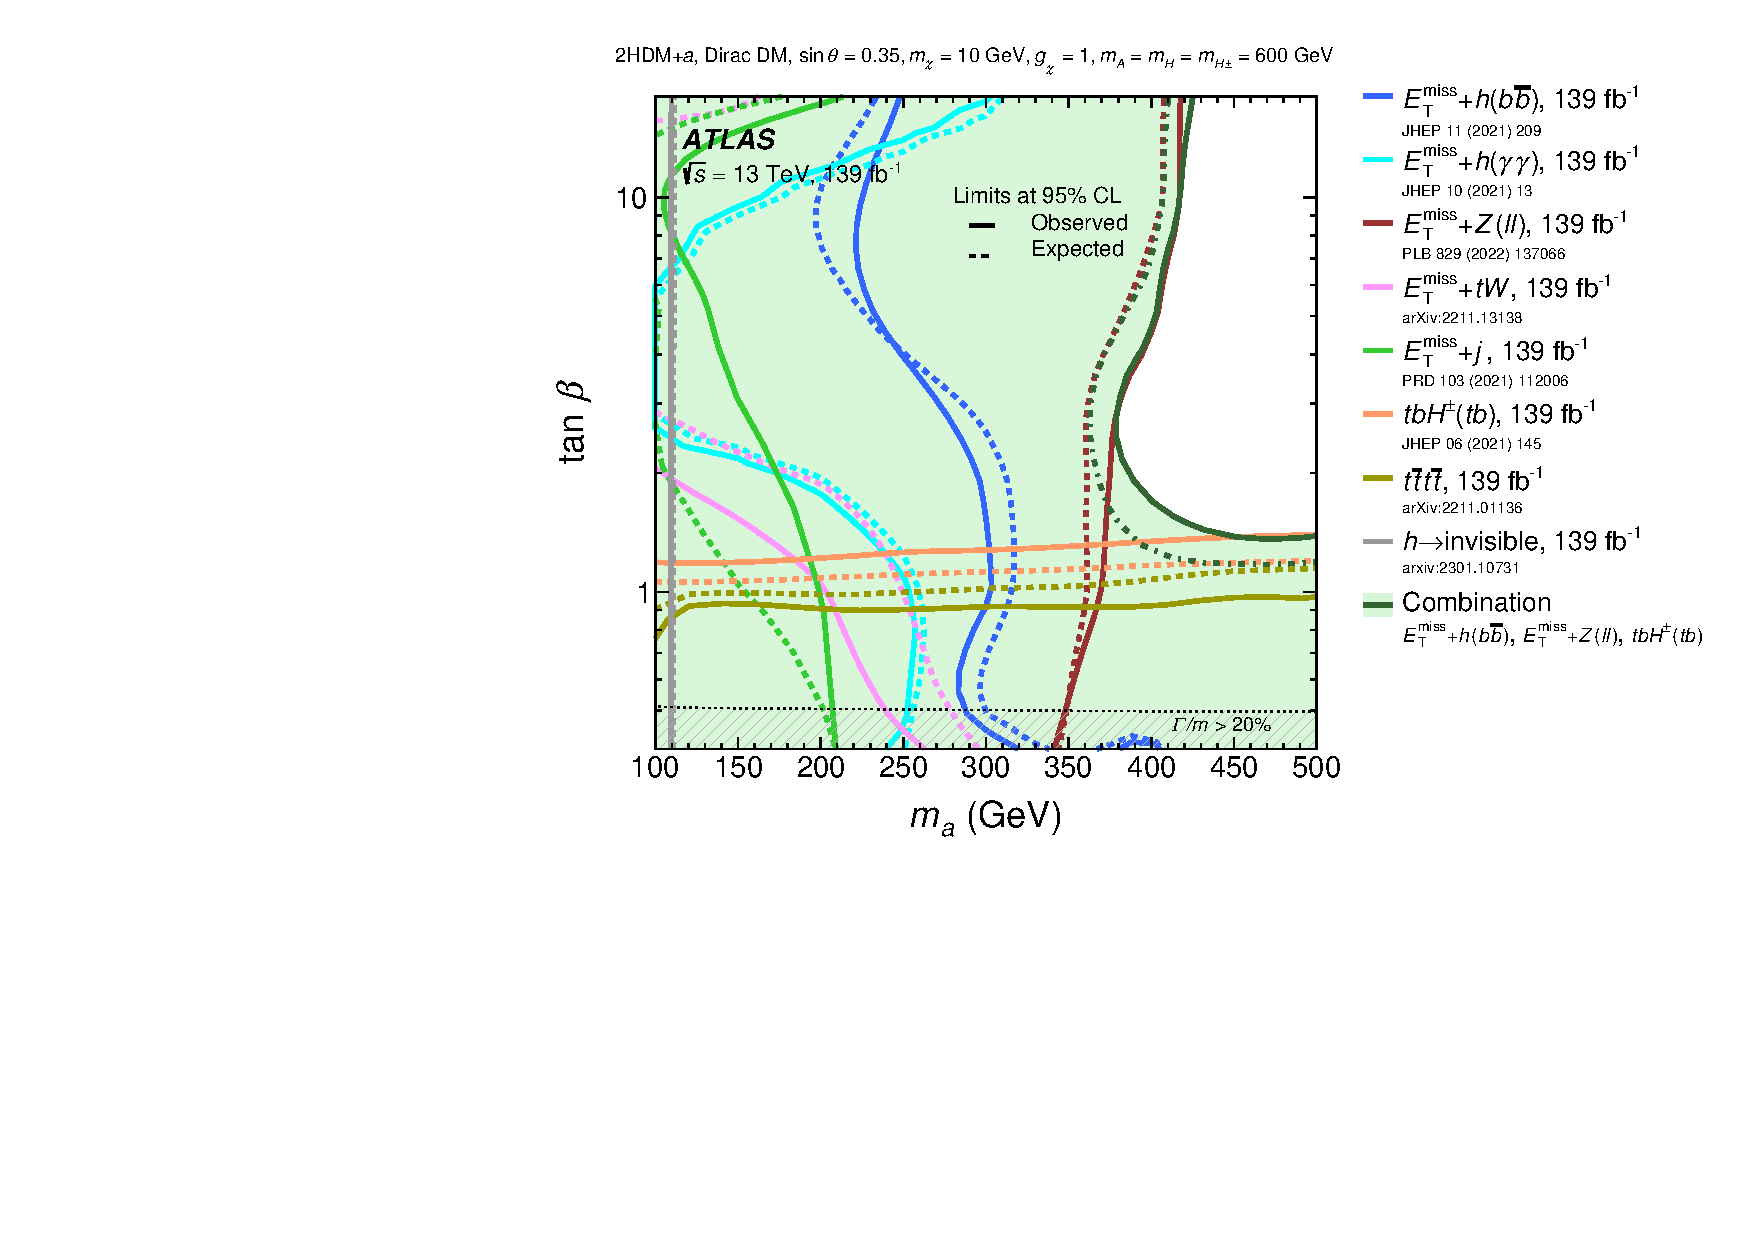
\includegraphics[width=\linewidth]{figures/fig_06a.pdf}
        \caption{}
        \label{fig:result-ma-tanb-scan-a}
    \end{subfigure}
    \begin{subfigure}[2]{0.495\textwidth}
        \centering
        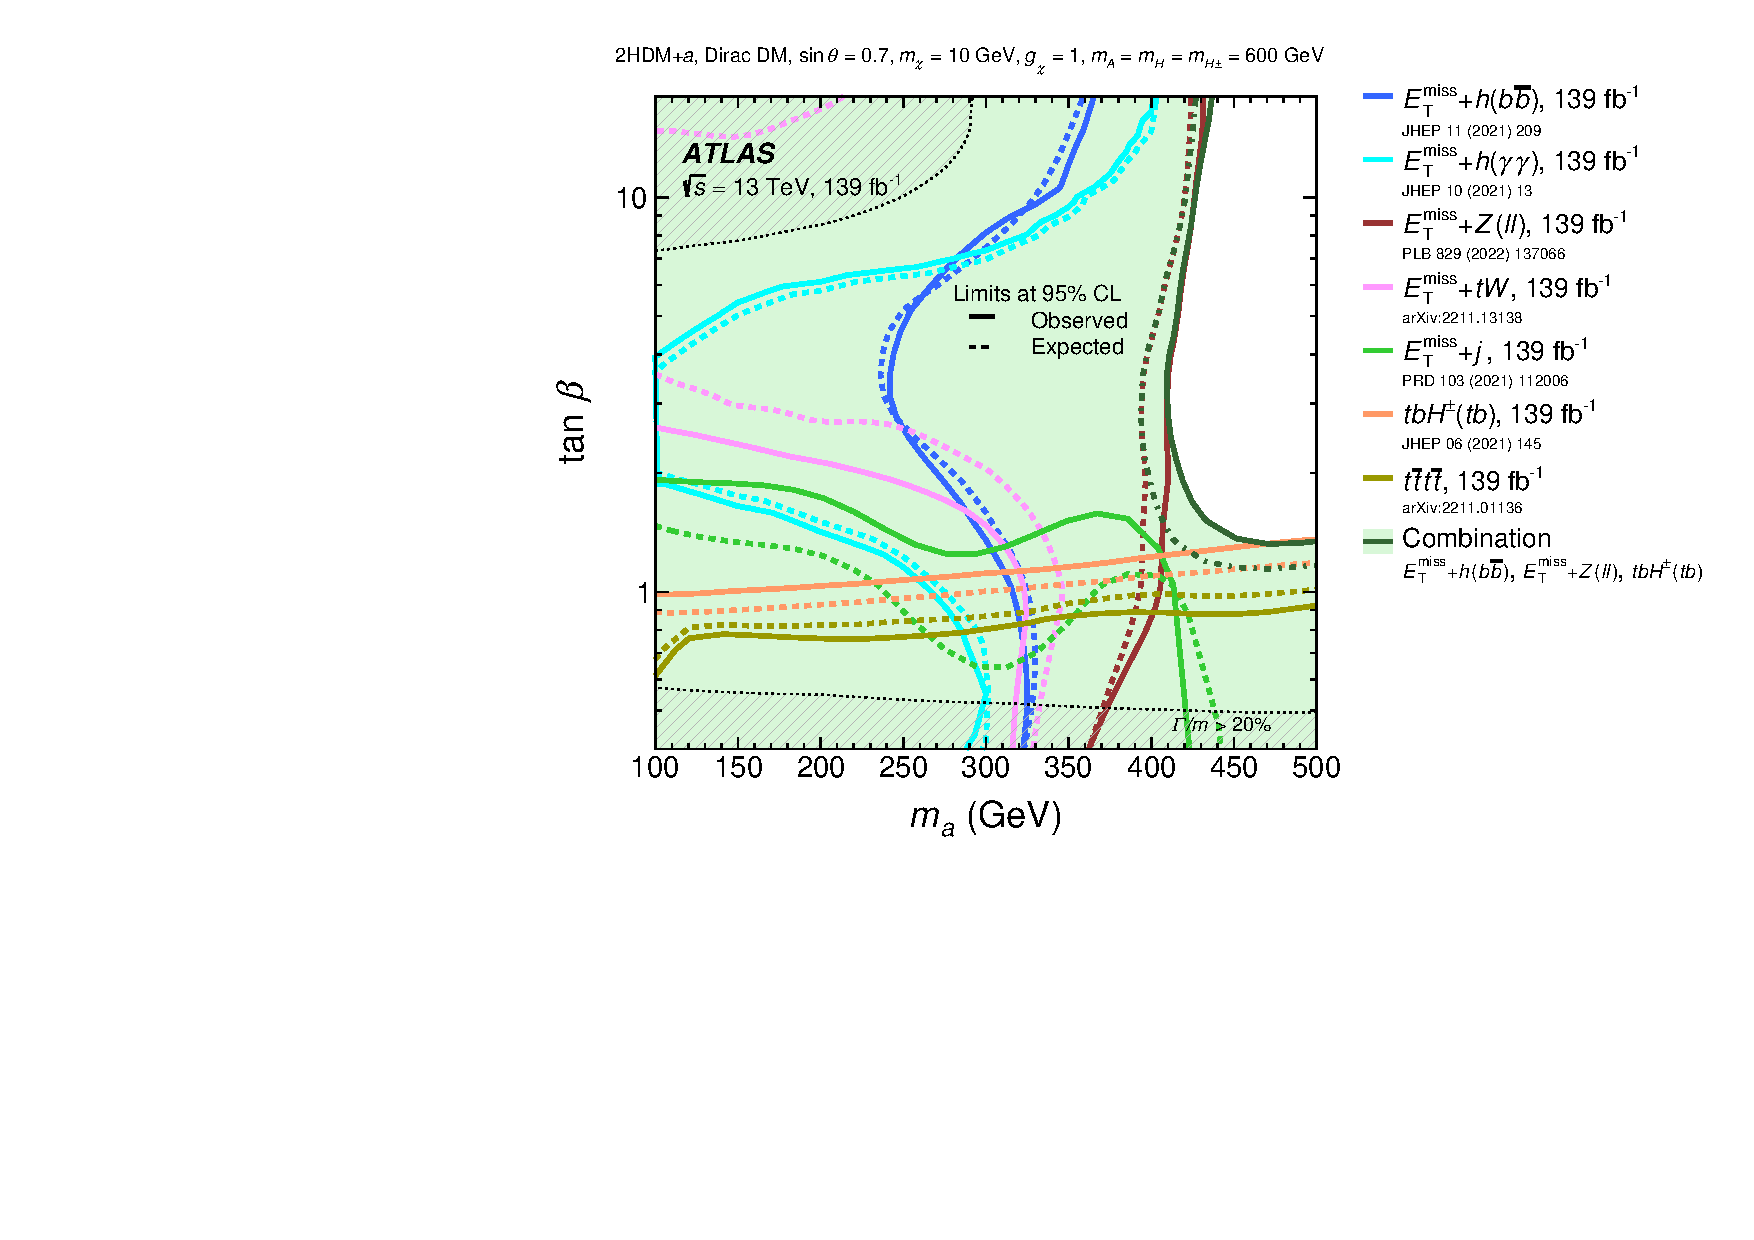
\includegraphics[width=\linewidth]{figures/fig_06b.pdf}
        \caption{}
        \label{fig:result-ma-tanb-scan-b}
    \end{subfigure}
    \caption{Observed and expected exclusion regions at $95\%$ CL over the $(m_a, \tanb)$ plane evaluated at \thdma mixing angles $\sint=0.35$ (a), and $\sint=0.7$ (b). The statistical combined contours are shown along with those from individual searches. In both subfigures, a dashed grey region indicates the region where the width of any of the Higgs boson exceeds $20\%$ of its mass. }
    \label{fig:result-ma-tanb-scan}
\end{figure} 

The $\met+tW$ search excludes regions of the parameter space at low $\tanb$ and low $m_a$. Better sensitivity is observed for the larger $A/a$ mixing angle. 

The $\met+j$ search excludes signal hypotheses characterized by low values of $m_a$ and $\tanb$, and its sensitivity is enhanced at $\sint=0.7$ due to more significant $a-A$ mixing, enlarging the signal cross-sections for $m_A>m_a$. 

The $\hinv$ decay suffers from small branching ratio and thus provides sensitivity at low values of $m_a$, independent of $\tanb$.

The $t\bar{t}t\bar{t}$ and $\htb$ searches constrain regions complementary to the $\met+X$ signatures. It is sensitive at low $\tanb$ and almost independent of $m_a$.

\subsection{Scenario 4: Variation of \texorpdfstring{$\sint$}{TEXT}}

Figure \ref{fig:result-sint-scan} summarizes the exclusion limits as a function of $\sint$ for the \thdma under both low- and high-mass mediator hypotheses. The upper row shows the results for the baseline parameter choice of Scenario 4, in which $\tanb=1.0$, and the lower row additional results obtained for alternative values of $\tanb$, namely $\tanb=0.5$ and $\tanb=50$. Exclusion limits shown in the subfigures on the left are derived at $m_A=600$ GeV, $m_a=200$ GeV, corresponding to scenario 4a and the low-mass hypothesis, and those on the right at $m_A=1.0$ TeV, $m_a=350$ GeV, corresponding to scenario 4b and the high-mass hypothesis. The exclusion limits are represented by the ratio of the excluded cross-section to the nominal cross-section of the signal model.

\begin{figure}[h!]
    \centering
    \begin{subfigure}[2]{0.495\textwidth}
        \centering
        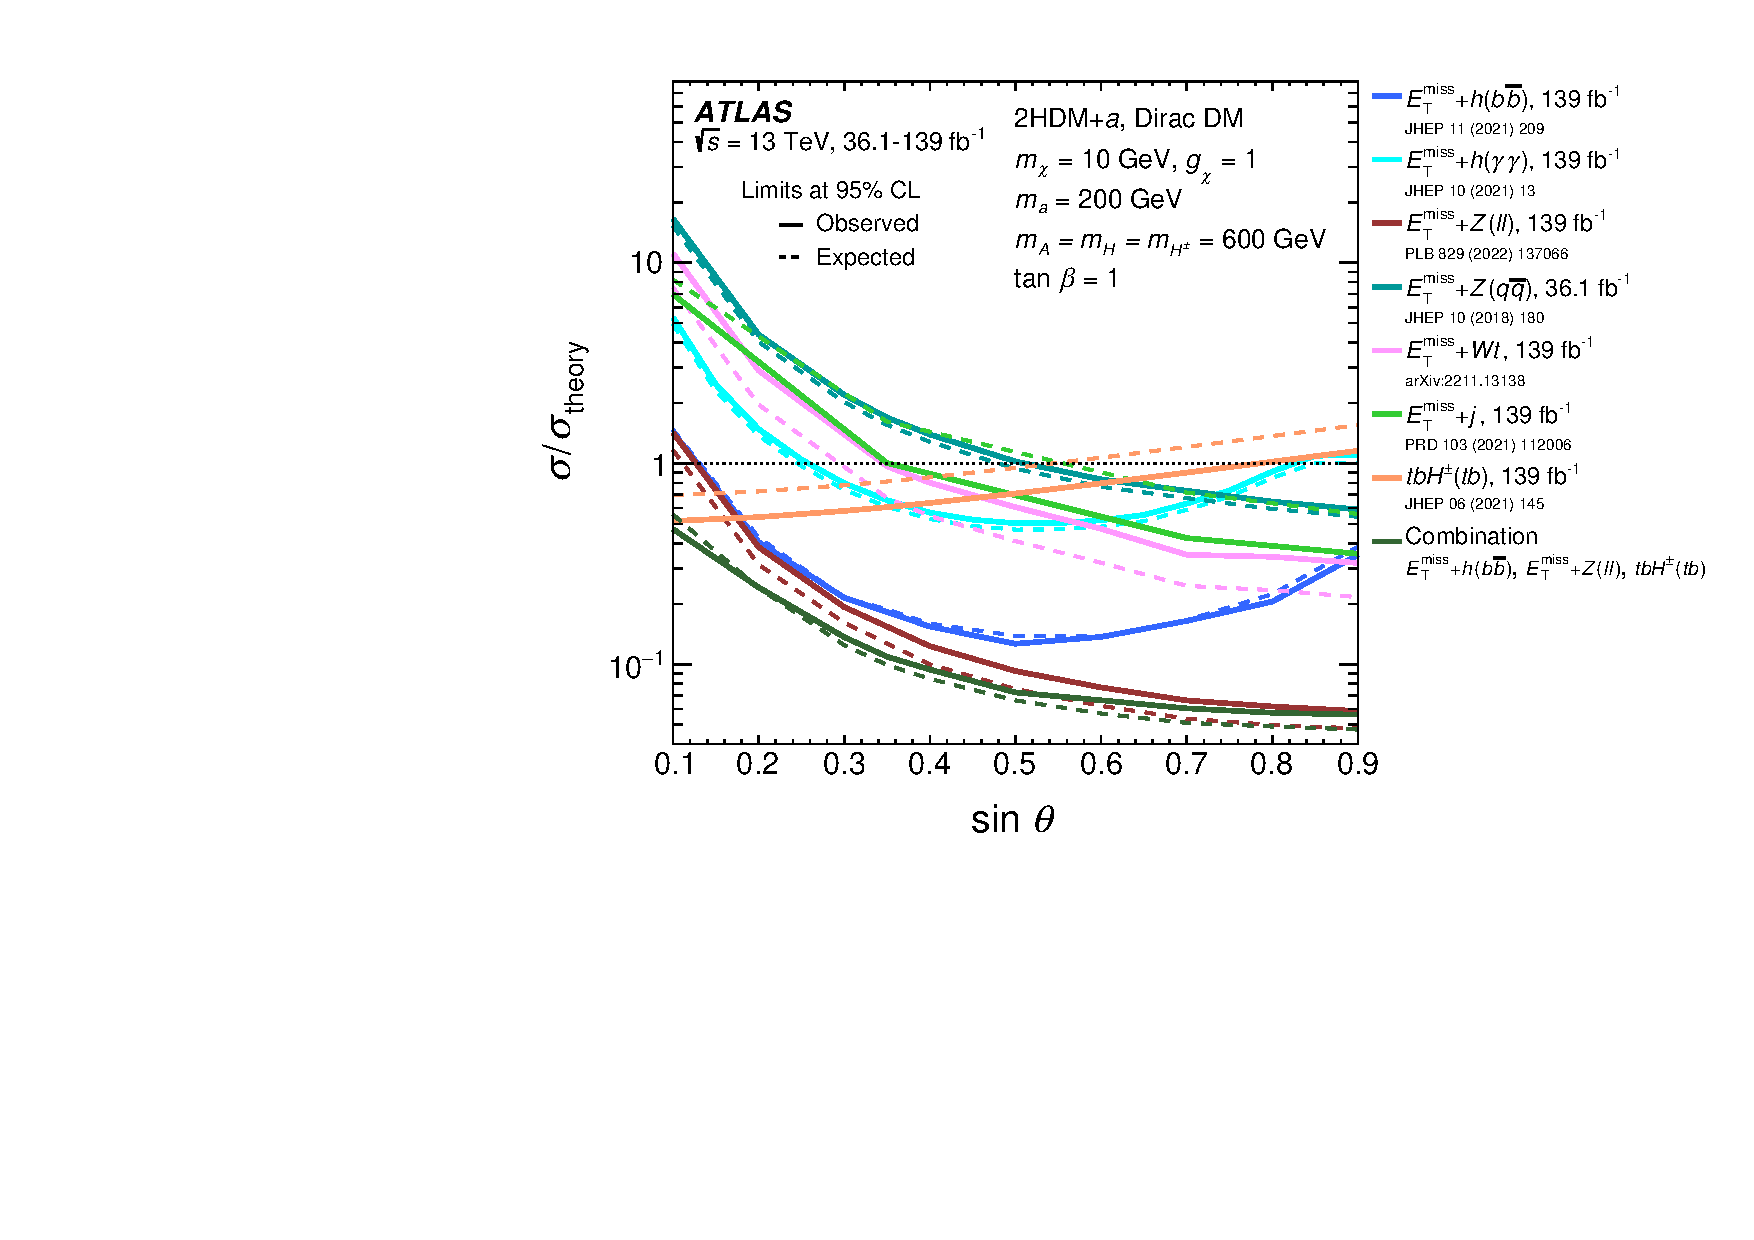
\includegraphics[width=\linewidth]{figures/fig_07a.pdf}
        \caption{}
        \label{fig:result-sint-scan-a}
    \end{subfigure}
    \begin{subfigure}[2]{0.495\textwidth}
        \centering
        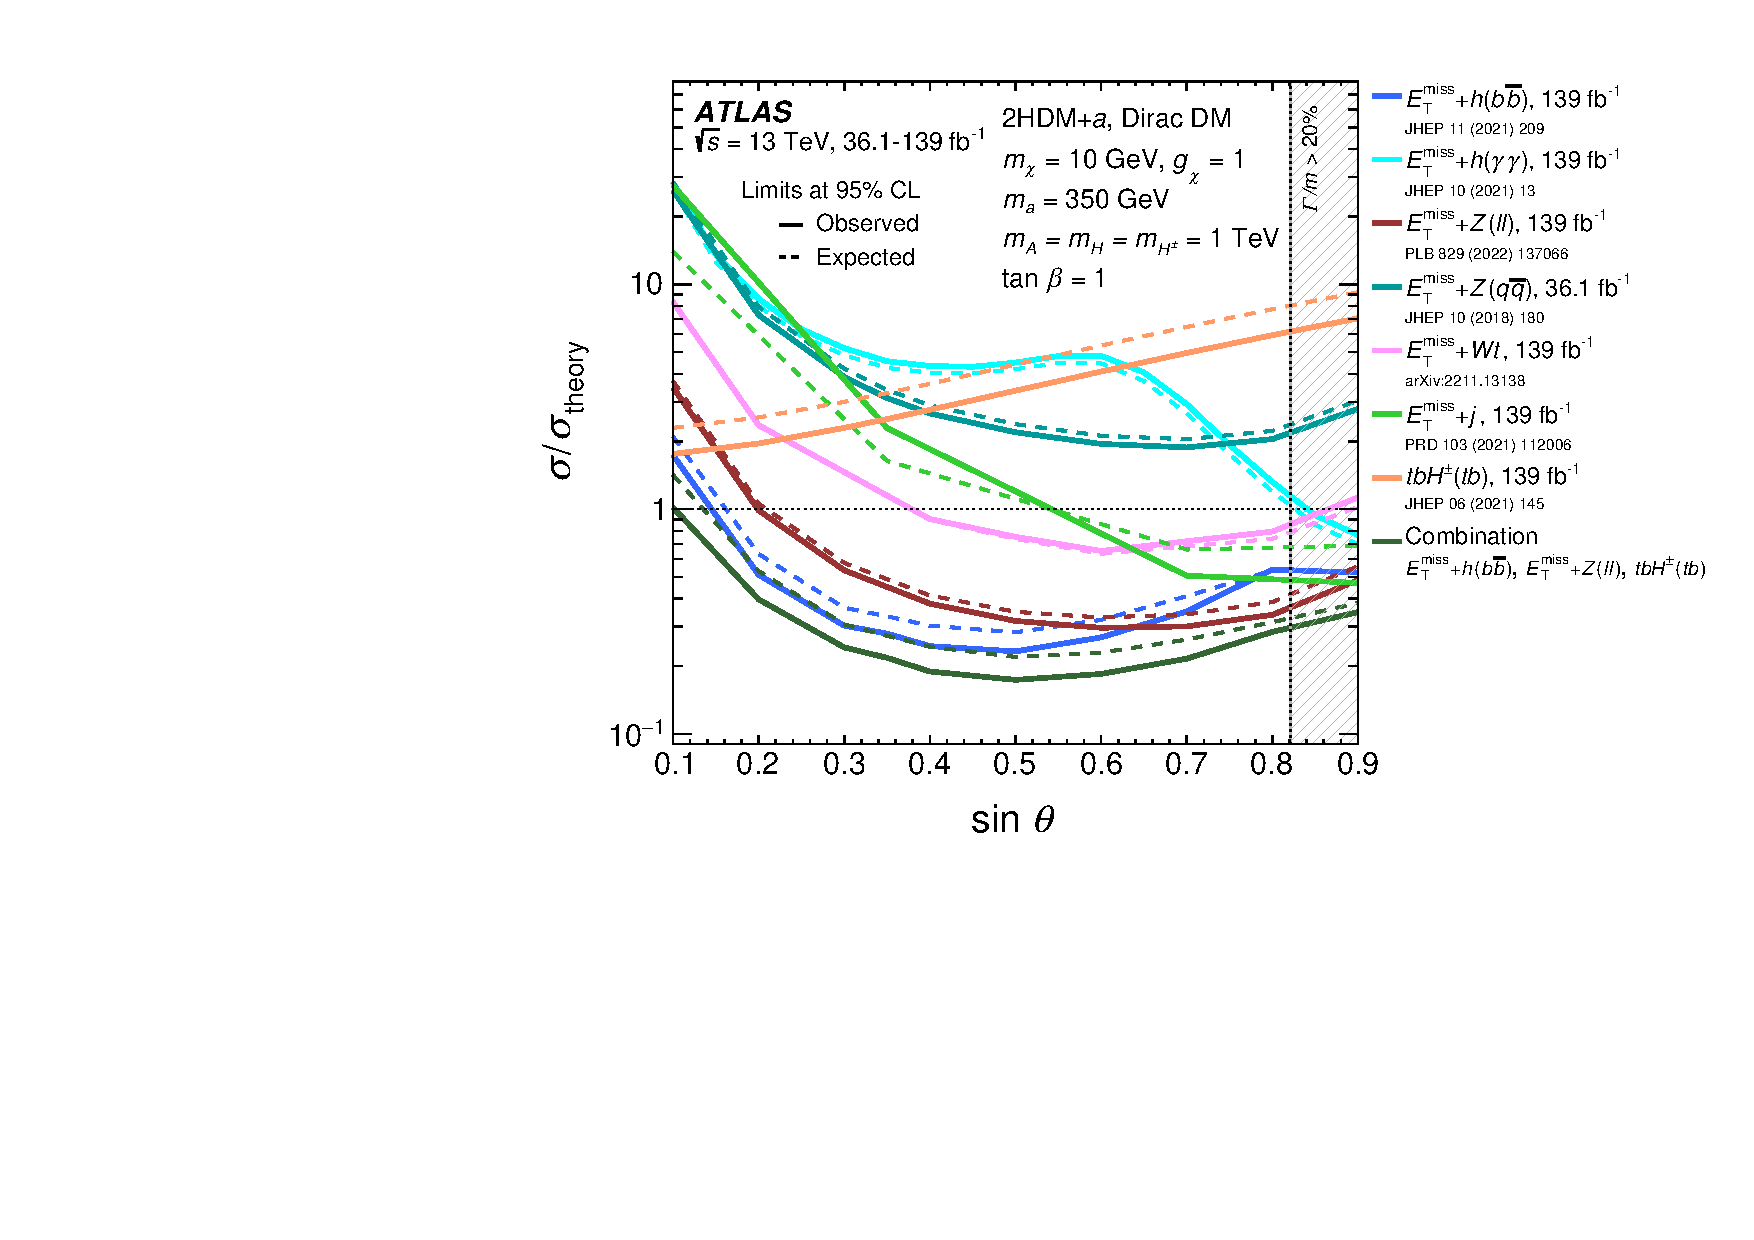
\includegraphics[width=\linewidth]{figures/fig_07b.pdf}
        \caption{}
        \label{fig:result-sint-scan-b}
    \end{subfigure}
    \begin{subfigure}[2]{0.495\textwidth}
        \centering
        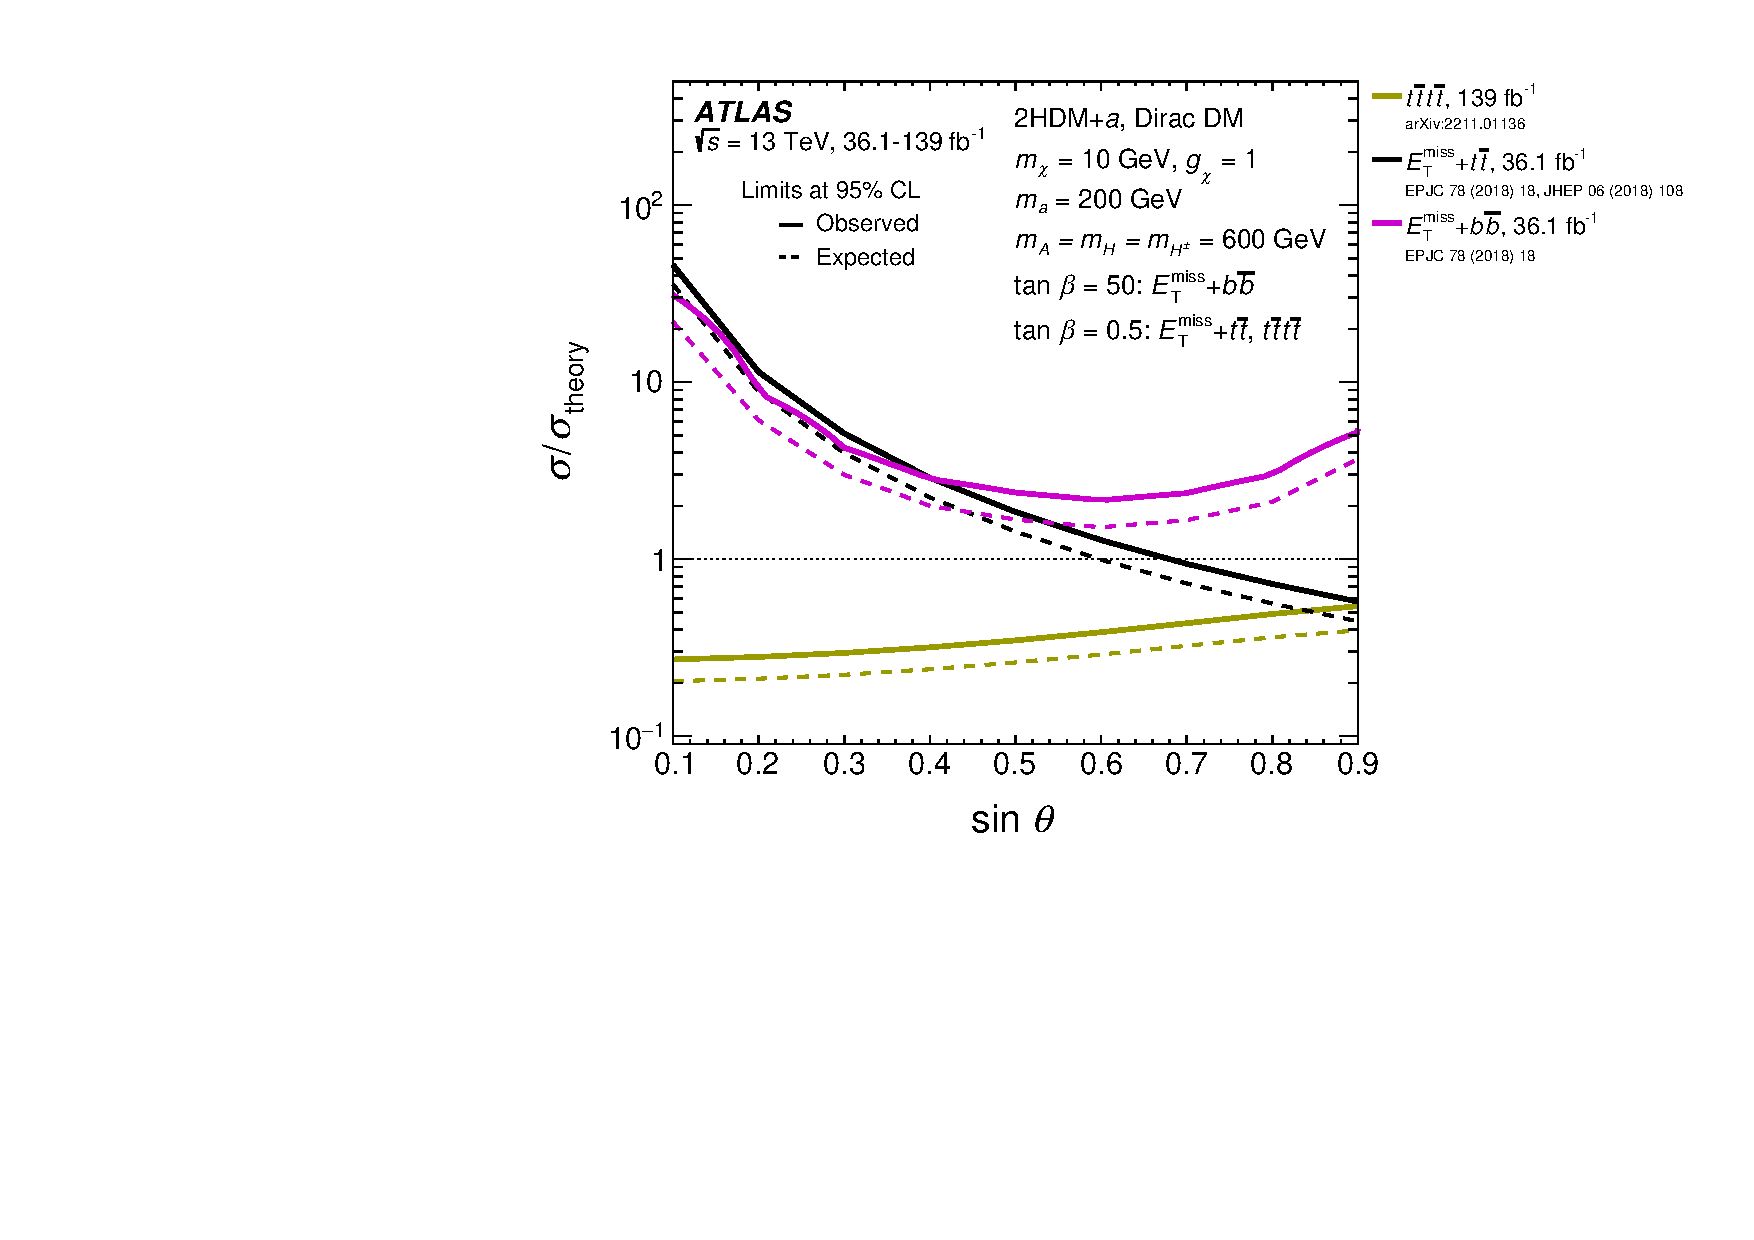
\includegraphics[width=\linewidth]{figures/fig_07c.pdf}
        \caption{}
        \label{fig:result-sint-scan-c}
    \end{subfigure}
    \begin{subfigure}[2]{0.495\textwidth}
        \centering
        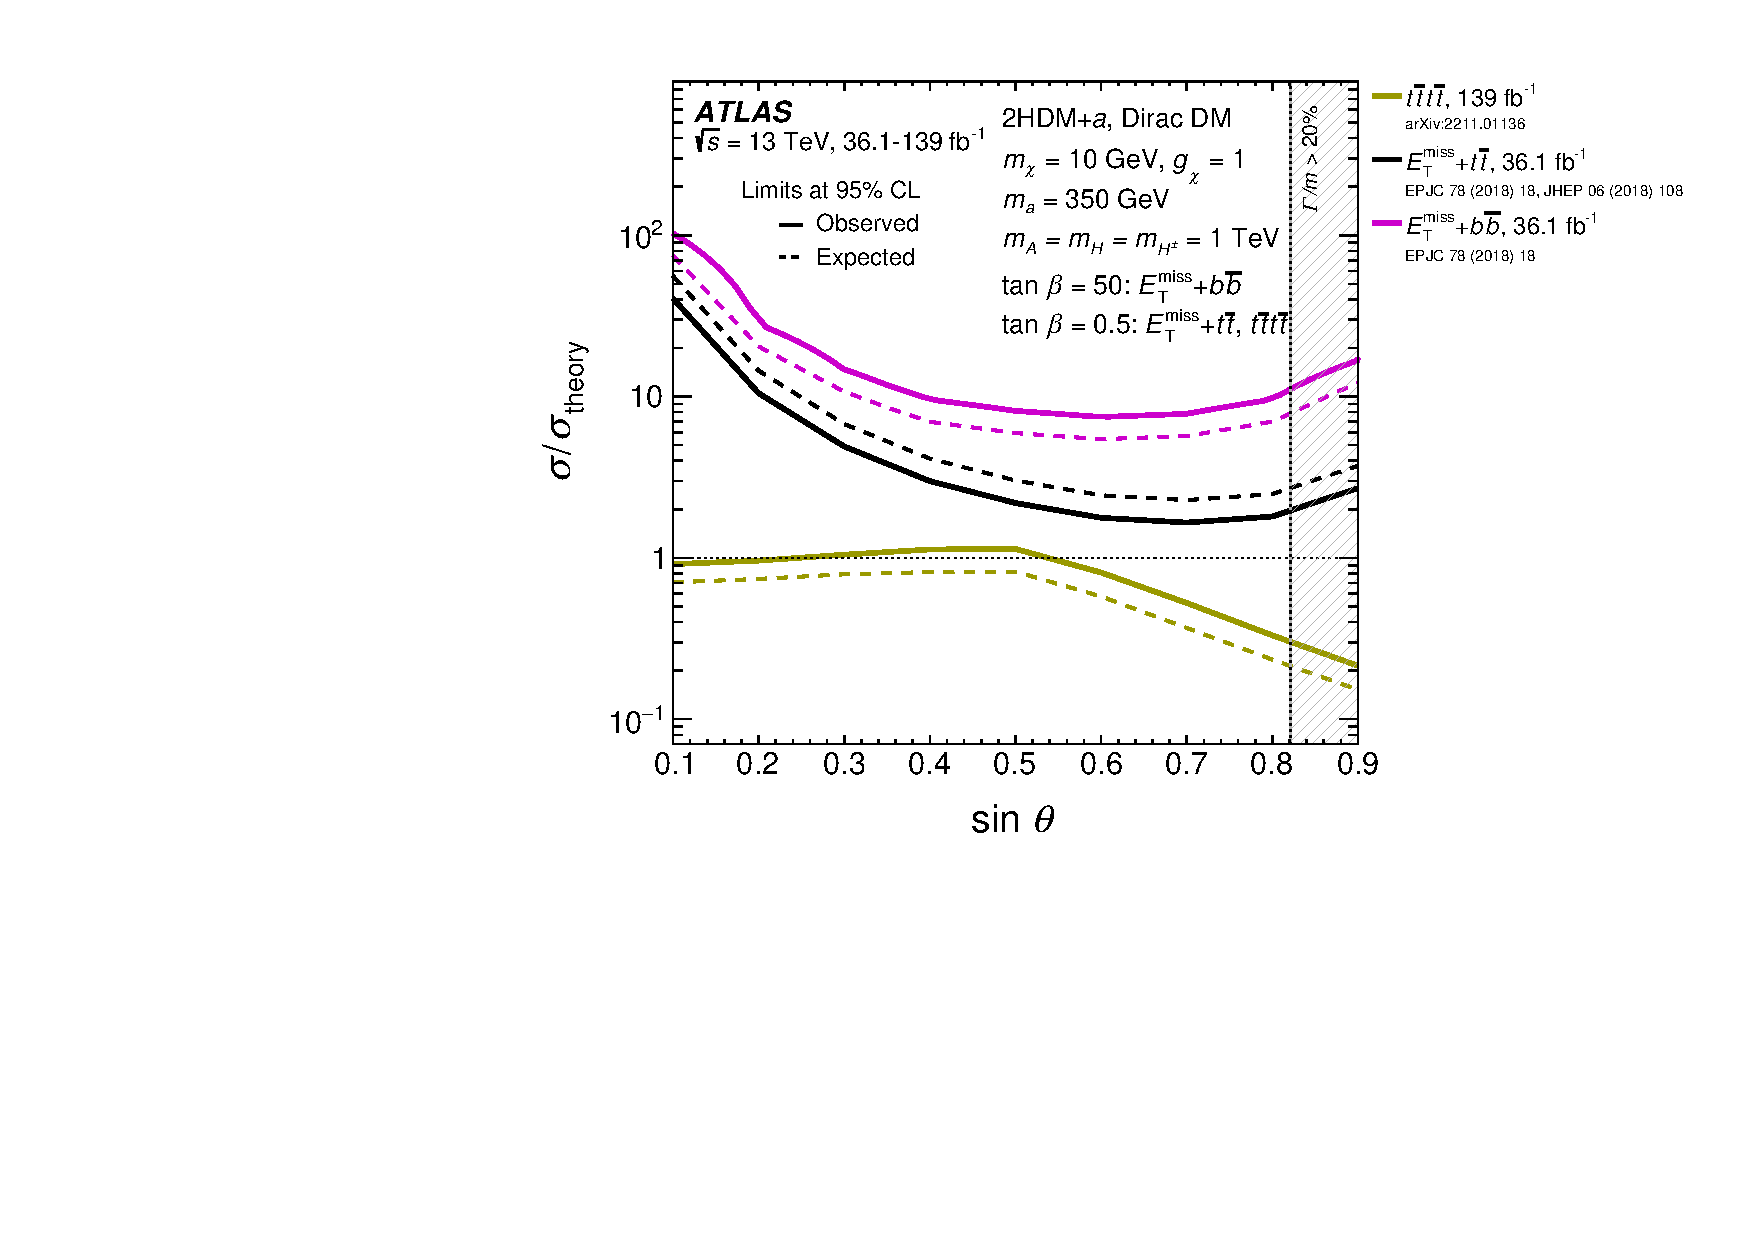
\includegraphics[width=\linewidth]{figures/fig_07d.pdf}
        \caption{}
        \label{fig:result-sint-scan-d}
    \end{subfigure}
    \caption{Observed and expected exclusion limits at $95\%$ CL for the \thdma as a function of $\sint$ plane evaluated under benchmark scenarios 4. In subfigures (a) and (b), the results are derived at $\tanb=1$, while in (c) and (d) they are derived at $\tanb=0.5$ or $\tanb=50$. (a) and (c) represent the sensitivity at low pseudo-scalar mass, in particular $m_A=600$ GeV and $m_a=200$ GeV, and (b) and (d) the high-mass regime, namely $m_A=1.0$ TeV and $m_a=350$ GeV. The combined exclusion is shown along with individual searches. In all subfigures, a dashed grey region indicates the region where the width of any of the Higgs boson exceeds $20\%$ of its mass. }
    \label{fig:result-sint-scan}
\end{figure} 

For the low-mass hypothesis at $\tanb=1.0$, the most stringent limits in the region of medium to high values of $\sint$ are set by the $\monozll$ and $\monohbb$ searches. The sensitivity of the former increases monotonically with $\sint$, as the cross-section of both non-resonant and resonant production mechanisms, illustrated in figures \ref{fig:hbb-signature} and \ref{fig:zll-signature}, grows with $\sint$. On the other hand, the production diagrams contributing to the $\met+h$ signature show a different dependence on $\sint$, as discussed in references \cite{Bauer:2017ota,EXOT-2017-32}. The relative contributions of each diagram are further affected by the different selections employed by the $\monohbb$ and \monohgamgam analyses, both of which reach a the maximum sensitivity around $\sint=0.5$. 

The sensitivity of both $\met+j$ and $\met+tW$ searches also monotonically increases with $\sint$, similar to that of the $\monozll$ signature, albeit an order of magnitude lower than the latter. This is due to the smaller cross-sections of these processes. Meanwhile, the $\htb$ and $t\bar{t}t\bar{t}$ signatures see a dependence on $\sint$ compared to other signatures, since they are not directly sensitive to neutral boson production. They are particularly sensitive at small mixing angle, with the sensitivity of $\htb$ exceeding that of the $\met+Z/h$ searches at $\sint < 0.2$. 

For the high-mass hypothesis at $\tanb=1.0$, the light pseudo-scalar mass is sufficiently large to kinematically allow the $a\rightarrow t\bar{t}$ decay, introducing an additional $\sint$ dependence in the interpretation of the $\met+Z/h$ searches. Consequently, the highest sensitivity for these analyses is observed near or just below the maximal mixing condition $\theta=\pi/4$. 

In the case of the $\met +h$ searches, there is a more complex dependence on $\sint$, owing to different contributions from the resonant and non-resonant productions of the Higgs boson to the final selection of each analysis. In particular, the $\met +h(b\bar{b})$ signature displays in a broad peak at values of $\sint$ slightly below the maximal mixing. In contrast, the $\met +h(\gamma\gamma)$ shows a local sensitivity minimum around $\sint\approx 0.6$. 

The $\met + tW$ search follows a similar $\sint$ dependence as the $\monozll$ and $\monohbb$ searches, but remains approximately an order of magnitude below the combined sensitivity. On the other hand, the $\met+j$ demonstrates a monotonic increase in sensitivity with $\sint$ and reaches a level similar to that of the $\monozll$ and $\monohbb$ searches at large $\sint$. Results from the $\met+V(q\bar{q})$ search are shown for completeness \cite{EXOT-2017-32}.

Alternative values $\tanb=0.5$ $\tanb=50$ are considered for Scenario 4 to illustrate the strong dependence of the exclusion limits on $\tanb$, particularly in searches that are sensitive to the Yukawa couplings of the neutral Higgs bosons and the mediator to fermions in a Type-II 2HDM. At low $\tanb$, the scalar and pseudo-scalar states couple primarily to top quarks, whereas at high $\tanb$, they predominantly couple to bottom quarks. Therefore, the results of the $t\bar{t}t\bar{t}$ search are shown for $\tanb=0.5$. The sensitivity of this search is generally higher in the low-mass scenario relative to the high-mass counterpart, mainly due to the reduced production cross-section of the heavy Higgs bosons $A/H$ at higher $m_{A/H}$. However, in the high-mass scenario, an enhancement in sensitivity is observed for $\sint > 0.5$, and attributed to the increased $a-A$ mixing and the fact that the mediator mass is sufficiently large to kinematically allow a decay into a pair of top quarks. At the same time, the mediator mass remains significantly below the masses of the heavy Higgs bosons, leading to the $t\bar{t}t\bar{t}$ signal cross-section being dominated entirely by $t\bar{t} + a (t\bar{t})$ production. 

For completeness, results from the $\met+t\bar{t}$ and $\met+b\bar{b}$ searches reported in Ref \cite{EXOT-2017-32} are included for $\tanb=0.5$ and $\tanb=50$, respectively.

\subsection{Scenario 5: Variation of \texorpdfstring{$\mchi$}{TEXT}}

In Figure \ref{fig:result-mX-scan}, the sensitivity of various searches as a function of the fermion dark matter mass $\mchi$, which has the strongest impact on the relic density predicted by the \hdma. The sensitivity is evaluated as the observed exclusion limit on the ratio of the excluded cross-section to the nominal cross-section of the signal model. The relic density is overlaid on the plot as a long-dashed line. A notable feature of the relic density occurs around $\mchi=m_a/2=200$ GeV, known as the $a$-funnel region, where the predicted density is depleted by the resonant enhancement of the process $\chi\bar{\chi}\rightarrow a\rightarrow \mathrm{SM}$ \cite{Djouadi:2005dz,Bagnaschi:2015eha,2HDMWGproxi}. A second resonant, occurring at $\mchi=m_A/2=500$ GeV, corresponding to a second funnel region, is not fully covered within the probed $\mchi$ range but nevertheless visible as a decrease in the predicted relic density for $\mchi >400$ GeV. For $\mchi >200$ GeV, the relic density plateaus due to the increase in annihilation cross-section of the DM particles near the kinematic threshold of the processes $\chi\bar{\chi}\rightarrow t\bar{t}$ (if $\mchi > m_t$) and $\chi\bar{\chi}\rightarrow ah$ (if $\mchi > (m_a+m_h)/2$). 

\begin{figure}[h!]
    \centering
    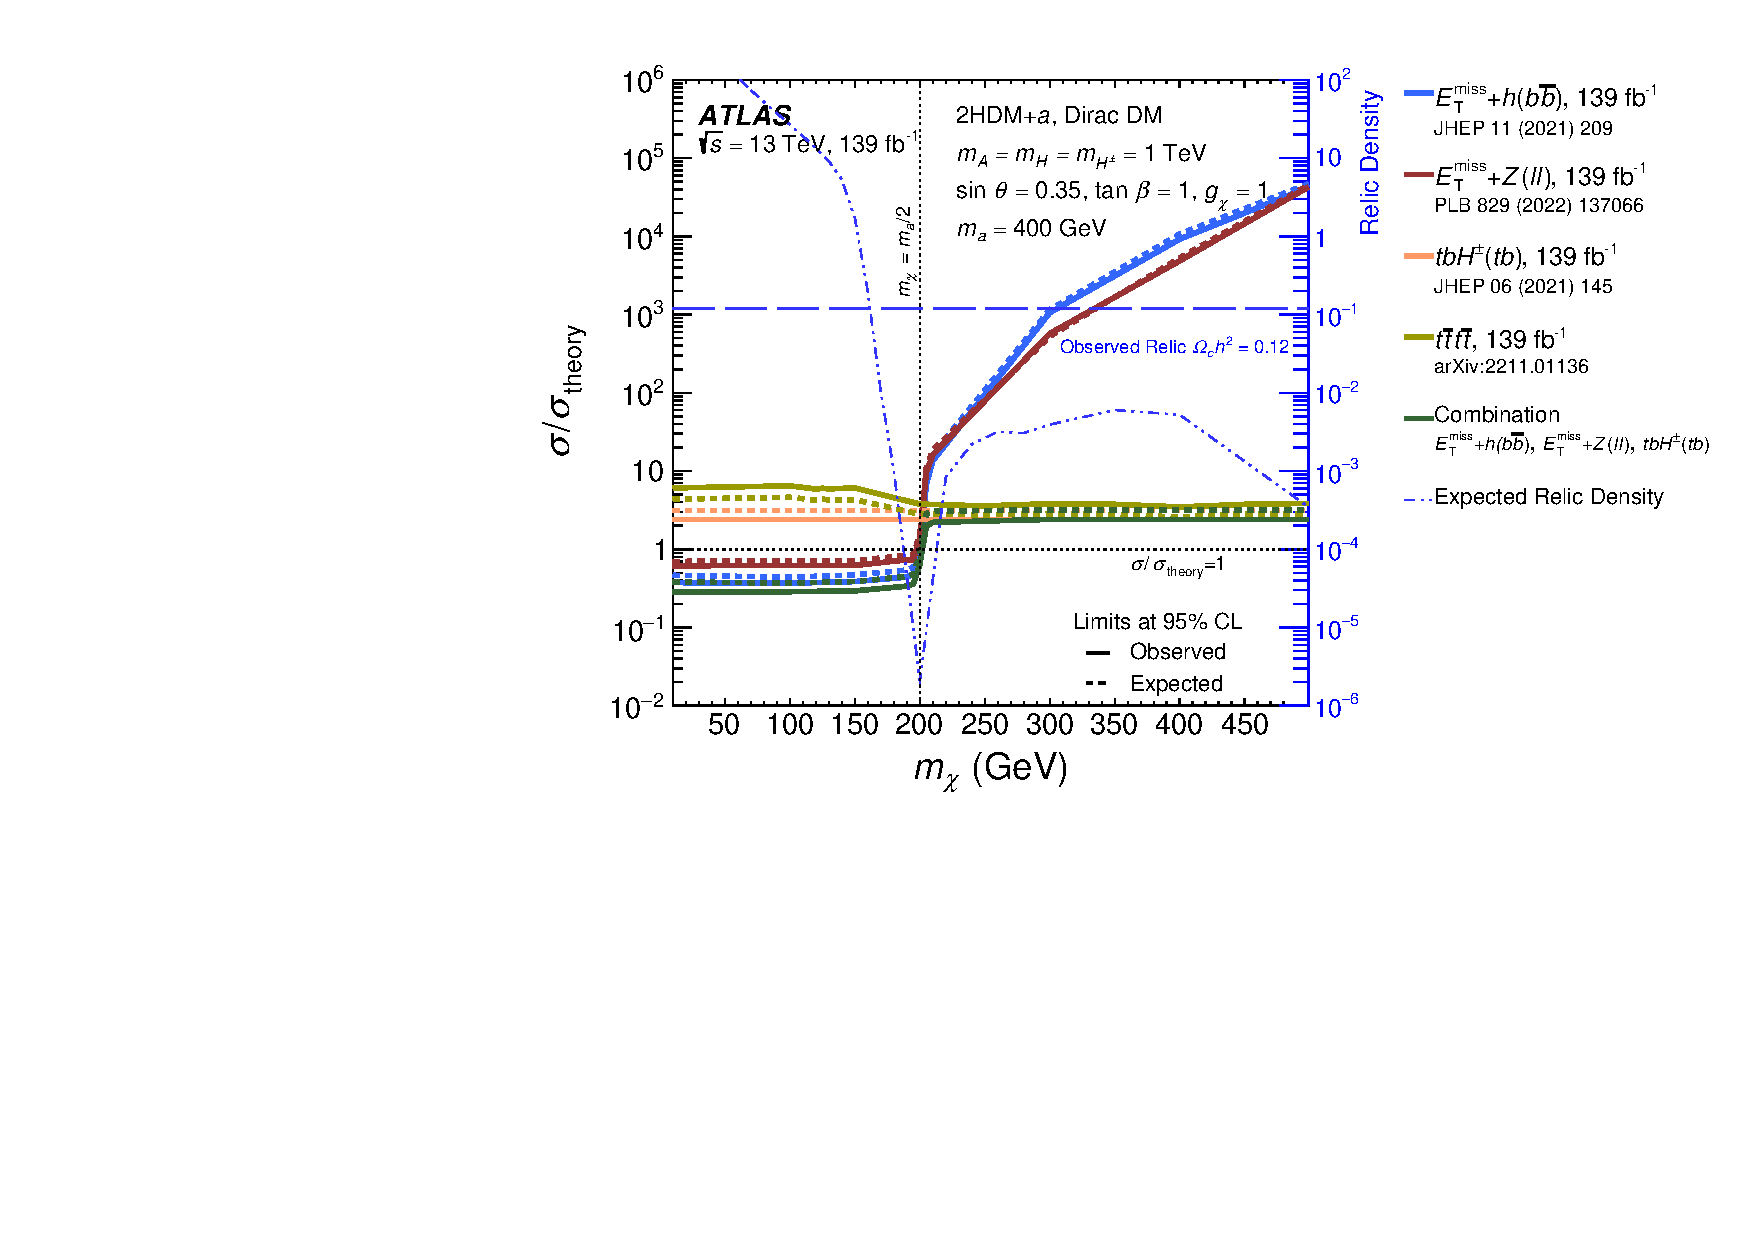
\includegraphics[width=0.6\linewidth]{figures/fig_08.pdf}
    \caption{Observed and expected exclusion limits at $95\%$ CL for the \thdma as a function of the dark matter particle mass $\mchi$ evaluated under benchmark scenario 5 following $m_A=1.0$ TeV, $m_a=400$ GeV, $\tanb=1.0$, and $\sint=0.35$. The limits are expressed in terms of the ratio of the excluded cross-section to the nominal cross-section of the signal model. The results from several individual searches are shown along with the combined limits. The relic density for each $\mchi$ assumption, calculated with \textsc{MadDM}~\cite{Ambrogi:2018jqj}, is superimposed on the plot in dashed line. }
    \label{fig:result-mX-scan}
\end{figure} 

For all considered signatures, the sensitivity becomes independent of $\mchi$ as long as the pseudo-scalar mediator, whose mass is fixed at 400 GeV in this benchmark scenario, can decay into a pair of DM particles. The most stringent constraints in the region where $\mchi<200$ GeV are provided by the $\monozll$ search. Together with the $\monohbb$, it excludes this part of the parameter space. However, at higher DM masses, the sensitivity of the $\met+Z/h$ searches rapidly decreases, while that of the $\htb$ and $t\bar{t}t\bar{t}$ searches remains largely constant. This is because the corresponding leading-order signal processes do not involve the DM particle $\chi$, rendering their signal cross-sections independent of $\mchi$. 

For $\mchi>m_a/2$, the $\htb$ search provides the strongest constraints, probing cross-sections as low as $\sigma =2\sigma_{\mathrm{theory}} - 3\sigma_{\mathrm{theory}}$. None of the searches exclude the \thdma in this mass range under the chosen benchmark scenario. It is possible to march the observed relic density for $\mchi=170$ GeV without changing the collider phenomenology, though this mass value is disfavored by the considered analyses. 

It is important to emphasize that the relic density considerations primarily serve as a tool to assess \thdma model predictions in the context of cosmological observations. They should not be interpreted as strict constraints on the model parameters, as the values of the parameters producing the correct relic density could shift if the model is modified to include additional physics at high-energy scales or if an alternative cosmological history is assumed.

\subsection{Scenario 6: \texorpdfstring{$m_a -\mchi$}{TEXT} plane}

Figure \ref{fig:result-ma-mX-scan} presents exclusion limits as a function of $m_a$ and $\mchi$ for Scenario 6. The $h\rightarrow aa \rightarrow f\bar{f}f'\bar{f}'$ searches target the region characterized by $m_a<m_h/2$ and $m_a < 2\mchi$, which kinematically allows the $h\rightarrow aa$ decay and forbids the $a\rightarrow \chi\bar{\chi}$ decay. This region is excluded almost entirely by these searches, except for two narrow bands where $m_a$ approaches the masses of the $J/\psi$ and $\Upsilon$ mesons. Searches for dimuon final states near the $J/\psi$ mass are experimentally challenging, as are searches for $h\rightarrow aa\rightarrow 4g$. The $\mu^+\mu^-\tau^+\tau^-$ final state provides some sensitivity but is not sufficient to exclude the higher mass range around $m_a=10$ GeV \cite{HIGG-2014-02}. Similarly, searches for hadronic final states are complicated by the collimation of the quark pairs, often necessitating dedicated techniques to enhance the sensitivity of signatures such as $b\bar{b}\gamma\gamma$ and $b\bar{b}b\bar{b}$. The $h\rightarrow aa \rightarrow f\bar{f}f'\bar{f}'$ searches lose sensitivity when $m_a>m_A/2$, as invisible mediator decays become dominant. For $m_a < m_h/2$, this region is excluded by the $\hinv$ search. For larger values of $m_a$, the region where $m_a>\mchi$ is excluded by the $\monohbb$  search up to $m_a\approx 600$ GeV. 

The remaining high-mass region is not excluded, and can be probed by searches targeting the mediator or heavy Higgs boson final states in $t\bar{t}t\bar{t}$ and $\htb$ signatures, which are currently unable to exclude $m_A=1200$ GeV.

\begin{figure}[h!]
    \centering
    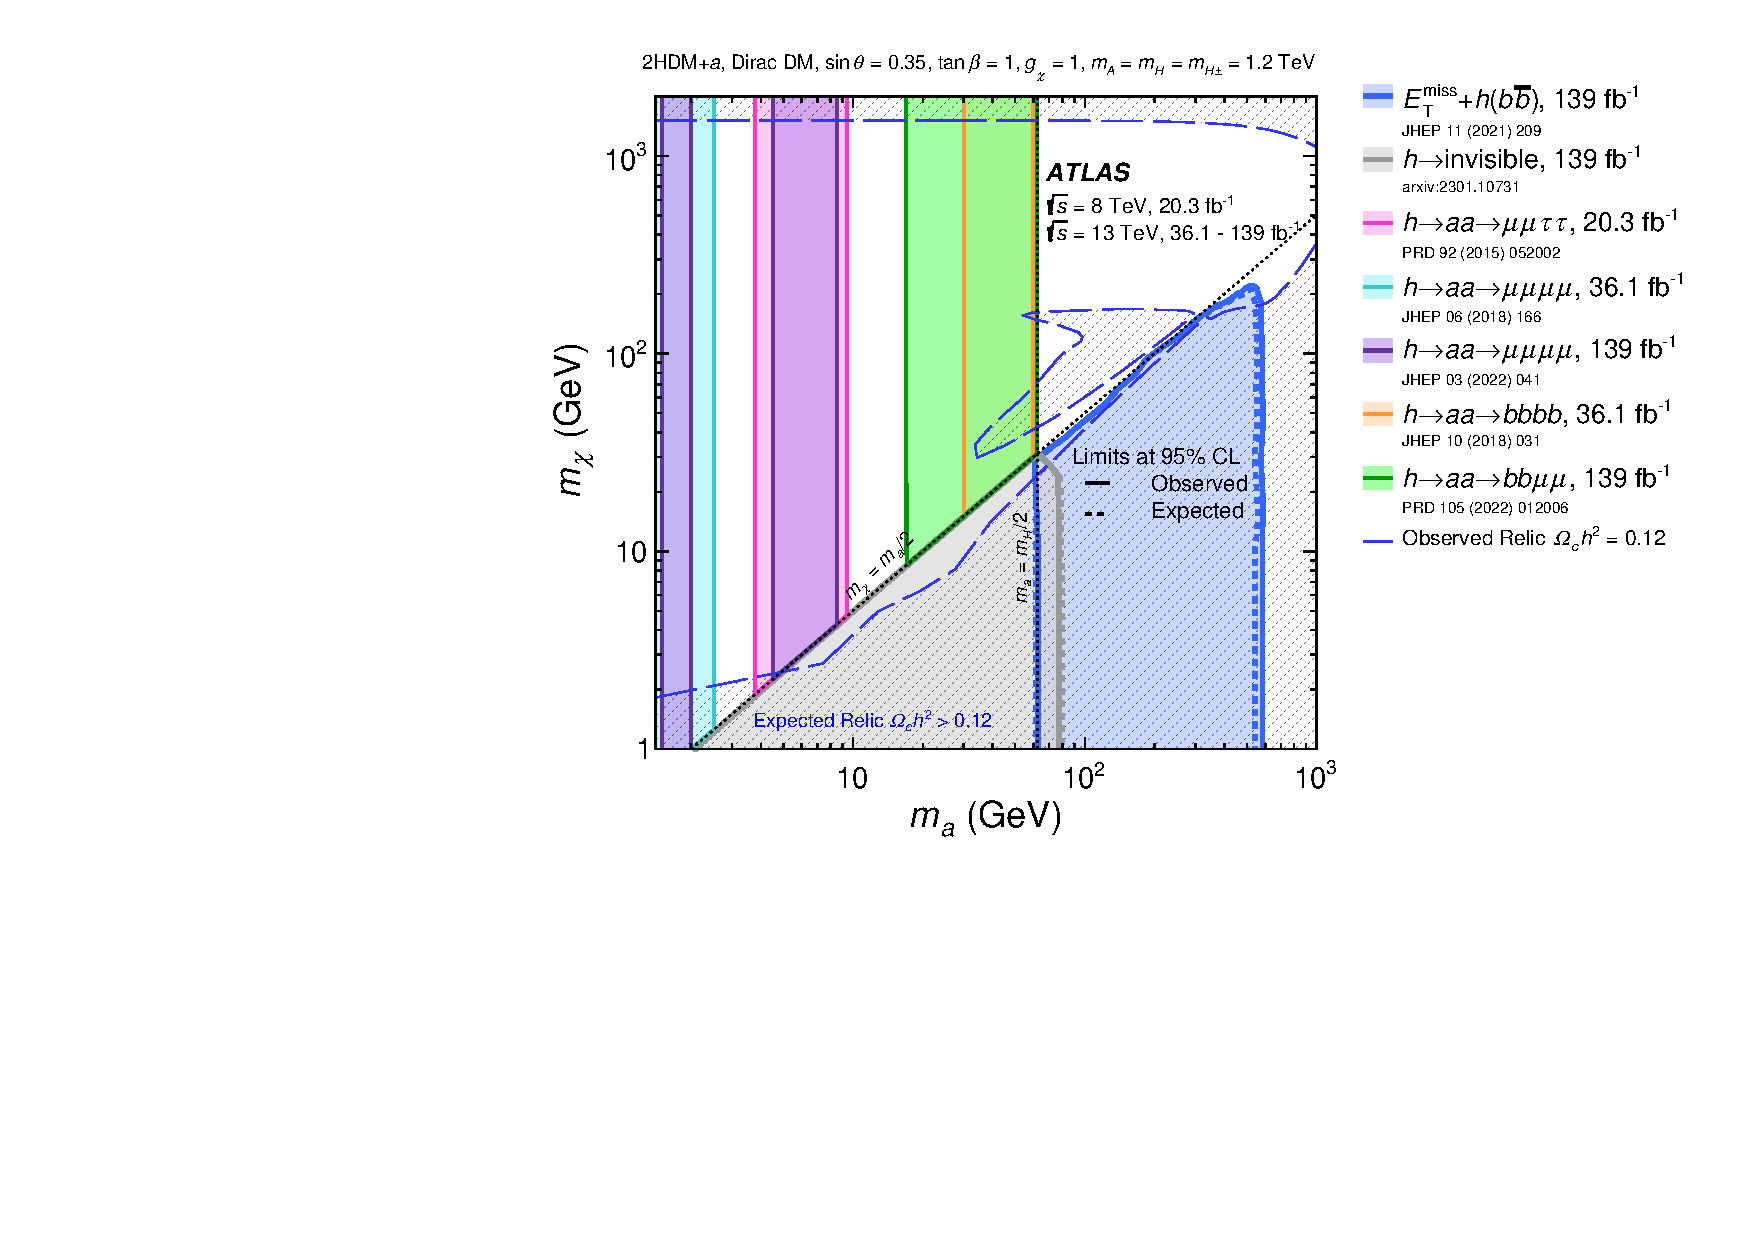
\includegraphics[width=0.6\linewidth]{figures/fig_09.pdf}
    \caption{Observed and expected exclusion limits at $95\%$ CL for the \thdma as a function of $m_a$ and $\mchi$ evaluated under benchmark scenario 6 following $m_A=1.2$ TeV, $\tanb=1.0$, and $\sint=0.35$. The relic density contour for the case $\Omega_ch^2=0.12$, calculated with \textsc{MadDM}~\cite{Ambrogi:2018jqj}, is superimposed on the plot in dashed line. The shaded regions mark the region where the model predicts a relic density greater than the observed value $\Omega_ch^2=0.12$. The island around $(\mchi\approx100, m_a\approx 100)$ GeV corresponds to the resonant enhancement of the process $\chi\bar{\chi} \rightarrow ah \rightarrow \mathrm{SM}$ that depletes the relic density. }
    \label{fig:result-ma-mX-scan}
\end{figure} 

The relic density contour for the case $\Omega_ch^2=0.12$ is overlaid on figure \ref{fig:result-ma-mX-scan} as a long-dashed line. Regions above this line at contour at low $\mchi$ and below it at high $\mchi$, with an exception of an island around $(\mchi\approx100, m_a\approx 100)$ GeV, have a predicted relic density $\Omega_ch^2 < 0.12$. 

Due to the strong Yukawa coupling, the annihilation $\chi\bar{\chi}\rightarrow t\bar{t}$ is highly efficient. However, in regions of small DM mass $(\mchi < m_t$, the decay is kinematically forbidden, often leading to an overabundance of relic density unless alternative annihilation mechanisms are available. Key processes that help deplete the relic density include resonant annihilation when $\mchi\approx m_a/2$, as well as other decay channels such as $\chi\bar{\chi}\rightarrow aa$, or $\chi\bar{\chi}\rightarrow ah$ when they are allowed or kinematically enhanced. For small mediator mass, annihilation into fermions, such as $b\bar{b}$, $c\bar{c}$, and $\tau\tau$ can be sufficiently efficient to compensate for their smaller couplings and deplete the relic density. Larger values of $\mchi$ can also satisfy the observed relic density, as these annihilations are suppressed. 

\section{Conclusion}

A wide range of searches for new phenomena performed by the ATLAS Collaboration are summarized and interpreted in the context of a Two-Higgs-Doublet model extended by a pseudo-scalar mediator $a$, designated \hdma. The model extends the Standard Model by introducing two Higgs doublets and an additional pseudo-scalar particle, which mediates interactions between dark matter and the SM particles. It predicts a wide variety of final states, of which the most relevant to DM searches consist of a large missing transverse energy originating from the decay of the mediator $a$ into DM particles and a mono-$X,\,(X=Z,h)$ visible signatures. The majority of searches considered in this summary are based on up to $139\,\ifb$ of proton-proton collision data at center-of-mass energy of $\sqrt{s}=13$ TeV collected by the ATLAS detector during the second run of the Large Hadron Collider. The results are in accordance with Standard Model predictions, as no significant excess is found. They are used to derive constraints on the \thdma for a diverse selection of benchmark scenarios recommended by the LHC Dark Matter Working Group previously explored, as well as several benchmark scenarios which provide insights into the rich phenomenology of the model. Three searches targeting $\monozll$, $\met+b(b\bar{b})$, and $\htb$ examine complementary regions of the parameter space, provide the most stringent constraints in many benchmark scenarios, and thus enter a statistical combination to derive an enhanced set of limits on the \hdma. 

All benchmark scenarios are simplified by assuming the mass degeneracy of the additional Higgs bosons, namely $m_A=m_{H^{\pm}}=m_H$. The combined result excludes masses of the pseudo-scalar mediator $a$ up to 560 GeV for $m_{A/H/H^{\pm}}=1.2$ TeV, $\sint=0.35$, and $\tanb=1.0$ (scenario 1a), and up to $640$ GeV for $m_{A/H/H^{\pm}}=2.0$ TeV, $\sint=0.7$, and $\tanb=1.0$ (scenario 1b). In regions of large heavy Higgs mass $(m_A)$, the $\monozll$ and $\met+b(b\bar{b})$ searches are the most sensitive. The results from this benchmark see a significant improvement over the same scan performed on $36\,\ifb$ of $\sqrt{s}=13$ TeV proton-proton collision data, which excludes values of $m_a$ up to 340 GeV for $m_{A/H/H^{\pm}}=1.0$ TeV, $\sint=0.35$, and $\tanb=1.0$. The improvement can be attributed to the full Run 2 dataset, as well as various improvements in the analysis strategies employed by individual searches, and a statistical combination of the most sensitive results.

The interpretation of the $\htb$ in the combined limits represents a novel strategy previously not considered. This signature is the most sensitive of the three combined searches in the low-$m_A$ region where $m_a>400$ GeV. It allows values of $m_A$ up to 650 GeV to be excluded across the entire range of examined $m_a$, highlighting the importance of searches not classically interpreted in the context of DM in constraining more complex models such as the \hdma. The statistical combination the $\monozll$, $\met+h(b\bar{b})$, and $\htb$ searches extends the sensitivity to the \thdma compared to that of individual analyses across different regions of the parameter space. In addition, the results of searches targeting $h\rightarrow aa \rightarrow f\bar{f} f'\bar{f}'$ are used for the first time to constrain a part of the parameter space not previously probed. Overall, these results represent the most comprehensive set of constraints on the \thdma obtained by the ATLAS collaboration to date.

